\chapter{Evaluation}
\label{chap:Evaluation}

Die Evaluation der entwickelten Interaktionsverfahren erfolgt in zwei Hauptabschnitten: einer technischen und einer inhaltsbasierten Evaluation. Ziel ist es, sowohl die technische Leistungsfähigkeit der Verfahren als auch deren Wechselwirkung mit den Inhalten zu analysieren. Im folgenden wird zunächst die technische Evaluation gefolgt von der inhaltsbasierten Evaluation beschrieben. Anschließend wird die Durchführung der Evaluation geschildert und die Ergebnisse werden vorgestellt. 

\section{Konzeption der Evaluation}

\subsection{Technische Evaluation}

Der technische Teil der Evaluation dient insbesondere der Überprüfung der Annahmen zu technischen Parametern wie Geschwindigkeit, Effizienz, Robustheit und Erlernbarkeit, die im Rahmen der Konzeption getroffen wurden. Darüber hinaus soll die gründsätzliche Usability der Verfahren evaluiert werden. Für jedes Verfahren wird ein spezifisches Szenario entwickelt, in dem die technischen Fähigkeiten der Verfahren in möglichst anspruchsvollen Situationen getestet werden. Die Szenarien sind in Bezug auf die verwendeten Elemente und die Anzahl der durchzuführenden Eingaben vergleichbar. Beide Szenarien bestehen aus zwei Abschnitten. Im ersten Abschnitt steht die einfache Selektion von Objekten im Vordergrund. Im zweiten Teil hingegen liegt der Schwerpunkt auf der Interaktion mit Dialogfeldern und damit auf der Interaktion auf verschiedenen Ebenen sowie auf der Selektion von Objekten, die räumlich nahe beieinander liegen. Ziel dieses Aufbaus ist es, möglichst viele Interaktionen zu generieren, um eine breite Datengrundlage zu erhalten. Darüber hinaus ermöglicht das Design die Beobachtung möglicher Lerneffekte bei den Testpersonen. Die Anordnung der Elemente innerhalb der Szenen ist absichtlich herausfordernd gestaltet, um insbesondere die Robustheit und Effektivität der Verfahren zu erproben. Darüber hinaus sind die Elemente über die gesamte 360°-Szene verteilt, um die Nutzung der Navigation zu forcieren. Im Folgenden werden die Herausforderungen, die bei der Anordnung der Elemente innerhalb der Szene berücksichtigt wurden, im Detail dargestellt. 

\textbf{Herausforderungen der Scanning-Verfahren}

Eine Herausforderung bei der Verwendung von Item Scanning ist zunächst eine hohe Anzahl von Elementen in der Szene, deren Reihenfolge im Scanning nicht unmittelbar ersichtlich ist. Dies erfordert ein aktives und konzentriertes Verfolgen der Reihenfolge, um das gewünschte Element auswählen zu können. Darüber hinaus wird die Positionierung von Elementen am Rand des Sichtfeldes als Herausforderung angesehen. Diese Elemente können von den Nutzenden leicht übersehen oder in der Scanreihenfolge nicht erwartet werden, was zu fehlerhaften oder unbeabsichtigten Selektionen führen kann. Darüber hinaus stellen längere Wartezeiten für Elemente, die erst spät in der Scanning-Reihenfolge erscheinen, eine weitere Herausforderung dar. Diese können zu Ungeduld und damit zu fehlerhaften Eingaben führen. Auch die Interaktion auf mehreren Ebenen, z.B. das Schließen von Pop-Ups oder das Navigieren in Dialogfeldern, wird als weitere Herausforderung angesehen.

Im Gegensatz dazu ist beim Cartesian Scanning die größte Herausforderung, das gewünschte Element bei nahe beieinander liegenden Elementen auszuwählen. Je näher die Elemente beieinander liegen, desto präziser muss die Selektion erfolgen. Dies erfordert dementsprechend ein genaues Timing und eine hohe Konzentration. Darüber hinaus wird auch bei diesem Scanning-Verfahren die Positionierung von Elementen am Rand des Sichtfeldes als Herausforderung angesehen. Insbesondere wenn sich Objekte weit oben oder weit links befinden, kann es schnell passieren, dass Nutzende die Selektion verpassen und auf einen weiteren Durchlauf der Selektionslinie warten müssen. Als letzte Herausforderung wird die Interaktion auf mehreren Ebenen gesehen. Insbesondere bei beweglichen Pop-Ups oder Menüs, die sich mit der Kopfposition im Sichtfeld bewegen, kann es schnell zu Verschiebungen und damit zu Fehleingaben kommen. Auch hier ist somit eine erhöhte Konzentration erforderlich. 

Die Szenarien für den technischen Teil der Evaluation werden so gestaltet, dass diese Herausforderungen gezielt getestet werden. Während im ersten Abschnitt die Positionierung der Elemente im Vordergrund steht, werden im zweiten Abschnitt die Nähe und die Ebenenstruktur der Objekte aufgegriffen. Zur Minimierung von Zufallseffekten wurde eine Mindestanzahl von fünf gleichartigen Objekten pro Szenario integriert.

\textbf{Fragestellungen und Datenerhebnung}

Durch den technischen Abschnitt sollen insbesondere folgende Fragestellungen zu den genannten Parametern beantwortet werden können:


\textit{Geschwindigkeit} 
    \begin{itemize}
        \item Wie lange dauert es, das Szenario zu durchlaufen? Begünstigt ein Verfahren einen schnelleren Durchlauf?
        \item Wie lang ist die Interaktionsgeschwindigkeit bei den Verfahren? Bietet ein Verfahren eine deutlich schnellere Interaktionsgeschwindigkeit?
        \item Gibt es Faktoren, die die Interaktionsgeschwindigkeit beeinflussen, etwa die Position der Objekte im Sichtfeld?
        \item Gibt es beim Cartesian Scanning deutliche Unterschiede in der Interaktionsgeschwindigkeit abhängig von der Position der Objekte?
        \item Führt eine schnellere Interaktionsgeschwindigkeit zu einer besseren Bewertung der Usability? 
    \end{itemize}
\textit{Robustheit}
    \begin{itemize}
        \item  Wie häufig treten Fehler bzw. unbeabsichtigte Eingaben bei den jeweiligen Verfahren auf? 
        \item Was sind die Gründe für auftretende Fehler?
        \item Wie häufig werden zwei oder mehr Durchgänge im Scanning benötigt?
        \item Wie häufig werden beim Cartesian Scanning leere Eingaben zur Korrektur von Fehlen verwendet? 
    \end{itemize}
\textit{Erlernbarkeit}
    \begin{itemize}
        \item Zeigt sich im Verlauf des Szenarios ein deutlicher Lerneffekt? 
        \item Wie entwickelt sich die Interaktionsgeschwindigkeit im Verlauf des Szenarios? 
        \item Reduziert sich die Anzahl der Fehler mit zunehmender Erfahrung?
    \end{itemize}
\textit{Usability}
    \begin{itemize}
    \item Wie wird die Usability der Verfahren bewertet?
    \item Gibt es deutliche Unterschiede in der Bewertung der Usability zwischen den beiden Verfahren? 
    \end{itemize}


Die Erfassung der technischen Daten erfolgt durch die Kombination von automatischem Logging direkt aus Unity und einem Evaluationsprotokoll. Es wird für jede durchgeführte Selektion die Interaktionsgeschwindigkeit ausgegeben. Außerdem wird die benötigte Zeit von Start bis Abschluss des Szenarios gespeichert. Fehler werden manuell gezählt und kategorisiert und zusätzliche Beobachtungen dokumentiert. Zur Evaluation der Usability wird die SUS in digitaler Form verwendet.

\textbf{Erwartete Ergebnisse der technischen Evaluation}

Die Erwartungen an die Verfahren basieren auf den theoretischen Überlegungen zur jeweiligen Methodik. Beim Item Scanning wird erwartet, dass es intuitiver und schneller erlernbar ist als das Cartesian Scanning. Dies könnte sich durch eine geringere Anzahl von Fehlern und selten erforderlichen Korrekturen zeigen. Allerdings wird das Item Scanning voraussichtlich bei der Navigation insgesamt langsamer sein, da größere Navigationen erforderlich sind, um alle platzierten Elemente erreichen zu können. Im Cartesian Scanning wird ein holpriger Start und eine entsprechend steilere Lernkurve erwartet. Es wird davon ausgegangen, dass die Navigation effizienter erfolgt und größere Winkel schneller abgedeckt werden. Herausforderungen wie eng beieinanderliegende Objekte oder solche am Rand des Sichtfelds könnten zu einer höheren Fehlerquote führen.

\subsection{Inhaltsbasierte Evaluation}

Der zweite Teil der Evaluation widmet sich der Wechselwirkung zwischen Interaktionsschnittstelle und Inhalt. Hier stehen die Parameter Komfort, Effizienz und visuelle Komplexität im Vordergrund. Die inhaltsbasierte Evaluation ergänzt den technischen Teil, indem die Verfahren in realistischeren Anwendungsszenarien getestet werden.
Es werden zwei Szenarien in Form einfacher Rätsel nach dem Prinzip von Escape Rooms erstellt. Die Aufgabe der Testpersonen besteht darin, einen hinter interaktiven Objekten wie Bildern oder Audiodateien versteckten Zahlencode zu ermitteln bzw. einen Schlüssel zur Lösung des Szenarios zu finden. Die Rätsel sind bewusst einfach gehalten, um die kognitiven Fähigkeiten der Testpersonen nicht zu fordern, da dies nicht im Fokus der Evaluation steht. Die Szenarien werden so gestaltet, dass sie realistische Bedingungen für die Nutzung der Interaktionsschnittstellen simulieren. Anzahl und Art der interaktiven Elemente sind in beiden Szenarien gleich, um die Vergleichbarkeit zu gewährleisten. Die Platzierung der Objekte erfolgt in Abstimmung mit den 360°-Videos der Szene. 

\textbf{Fragestellungen und Datenerhebnung}

Ziel der inhaltsbasierten Evaluation ist es, die folgenden Aspekte zu untersuchen:

\textit{Ablenkung durch die Verfahren}
\begin{itemize}
    \item Werden die Interaktionsschnittstellen als störend empfunden?
    \item Lenken die Interaktionsschnittstellen die Aufmerksamkeit der Testpersonen vom Inhalt ab?
\end{itemize}
\textit{User Experience}
\begin{itemize}
    \item Wie wird die User Experience der Verfahren bewertet?
    \item In welchen Faktoren treten (deutliche) Unterschiede in der Bewertung zwischen den Verfahren auf? 
    \item Decken sind die subjektiven Angaben hinsichtlich der Effizienz mit den gemessenen technischen Daten?
\end{itemize}
\textit{Motion Sickness}
\begin{itemize}
    \item Tritt Motion Sickness auf? Wenn ja, wie stark sind die Symptome ausgeprägt?
    \item Welche Symptome treten auf vermehrt auf?
    \item Gibt es Unterschiede zwischen den Verfahren in Bezug auf die Häufigkeit und Intensität der Symptome?
    \item Bestehen Korrelationen zwischen dem Auftreten von Motion Sickness Symptomen und der Bewertung der Usability/UX sowie der Interaktionsgeschwindigkeit? 
\end{itemize}

Die Erhebung der Daten erfolgt über standardisierte Fragebögen. Zur Messung der UX wird der User Experience Questionnaire (UEQ) verwendet. Der Simulator Sickness Questionnaire (SSQ) erfasst Symptome von Motion Sickness. Um Aussagen hinsichtlich der Ablenkung und Presence tätigen zu können, werden zusätzlich spezifische Fragen zur Wechselwirkung zwischen Interaktion und Inhalt gestellt. Diese werden in Anlehnung an Fragen aus dem Presence Questionnaire formuliert. Die gestellten Fragen lauten dabei:

\begin{itemize}
    \item Wie sehr warst Du in die Erfahrung der virtuellen Umgebung involviert?
    \item Wie gut konntest Du Dich auf die zugewiesenen Aufgaben oder erforderlichen Tätigkeiten konzentrieren und nicht auf die Mechanismen, die zur Ausführung dieser Aufgaben oder Tätigkeiten genutzt werden?
    \item Wie gut konntest Du Dich auf den Inhalt und die visuellen Darstellungen in der Szene konzentrieren?
\end{itemize}

Zusätzlich wird auch für das inhaltsbasierte Szenario ein automatisierter Log erstellt. Auch hier werden, wie zuvor im technischen Szenario, Daten zur Geschwindigkeit erfasst. Auch Fehler werden weiterhin im Evaluationsprotokoll vermerkt. 

Die erhobenen Daten werden statistisch ausgewertet. Für den UEQ werden die Ergebnisse mit dem Auswertungstool der Autoren analysiert. Für den SSQ werden die Ergebnisse nach der Methode der Entwickler ausgewertet und die entsprechenden SSQ-Scores ermittelt. Zusätzliche Fragen werden mit Hilfe von Mittelwerten und Standardabweichungen interpretiert, um Einblicke in spezifische Aspekte wie z.B. die inhaltliche Fokussierung zu erhalten.

Es wird erwartet, dass das Item Scanning aufgrund der geringen Anzahl von Elementen in den jeweiligen Szenen schneller ist und daher hinsichtlich der UX besser bewertet wird, insbesondere hinsichtlich Effizienz. Beide Verfahren sollten eine geringe Ablenkung vom Inhalt aufweisen und nur minimal zur Entstehung von Motion Sickness beitragen.

\section{Durchführung}

Die Evaluation der entwickelten Interaktionsschnittstellen wurde im Zeitraum vom 11. bis 15. Dezember 2024 an der Technischen Hochschule Lübeck durchgeführt. Insgesamt nahmen 16 Personen (10 männlich, 5 weiblich, 1 nicht-binär) ohne motorische Beeinträchtigungen an der Evaluation teil. Obwohl die Teilnehmenden nicht aus der primären Zielgruppe rekrutiert wurden, liefert ihre Teilnahme wertvolle Informationen über die Funktionalität und Benutzerfreundlichkeit der Implementierungen. Die Auswahl einer heterogenen Gruppe ohne motorische Beeinträchtigungen ermöglicht eine Bewertung der allgemeinen Nutzbarkeit der Verfahren. Darüber hinaus können potenzielle Schwachstellen in der Interaktion und technische Herausforderungen unabhängig von spezifischen Beeinträchtigungen identifiziert werden. Dies schafft eine solide Basis für weitere Optimierungen und ermöglicht es, die Implementierungen so anzupassen, dass sie zukünftig sowohl für die Zielgruppe als auch für einen breiteren Kreis von Nutzenden geeignet sind.

Jede Evaluationssitzung folgte einem standardisierten Ablauf und dauerte zwischen 45 und 60 Minuten pro Person. Der genaue Ablauf gliederte sich wie folgt:

{\normalfont \bfseries 1. Einführung:}

Die Teilnehmenden wurden begrüßt und in das Projekt, das Ziel der Evaluation und den Ablauf eingeführt. Die VR-Brille wurde auf die Person eingestellt (Größe und Abstand der Linsen). 

{\normalfont \bfseries 2. Abfrage des gesundheitlichen Zustands:}

Vor Beginn der eigentlichen Tests wurden die Teilnehmenden befragt, ob sie Symptome wie z.B. Kopfschmerzen, Schwindel oder Übelkeit verspürten. Damit sollte sichergestellt werden, dass mögliche Symptome von Motion Sickness nicht bereits vor der Nutzung der Anwendung vorhanden waren und die Ergebnisse des Fragebogens zuverlässiger ausgewertet werden können. 

{\normalfont \bfseries 3. Erklärung des ersten Interaktionsverfahrens:}

Die Funktionsweise des ersten zu testenden Scanning-Verfahrens wurde erläutert. Es wurde erklärt, wie das Scanning gestartet werden kann und wie Selektion und Navigation funktionieren. 

{\normalfont \bfseries 4. Durchführung der technischen Evaluation:}

Nach der Erklärung des Scanning-Verfahrens folgte eine kurze Erläuterung der Aufgabe im technischen Szenario, die dann von den Teilnehmenden durchgeführt wurde. Anschließend nahm die Testperson die VR-Brille ab und füllten den ersten Fragebogen (SUS) in digitaler Form aus. 

{\normalfont \bfseries 5. Durchführung der inhaltsbasierten Evaluation:}

Nach dem Ausfüllen des Fragebogens wurde den Teilnehmenden die Aufgabe des inhaltsbasierten Szenarios erklärt und dieses durchlaufen. Anschließend wurden die restlichen Fragebögen (UEQ, SSQ), ebenfalls in digitaler Form, ausgefüllt.

{\normalfont \bfseries 6. Wechsel zum zweiten Verfahren:}

Die gleiche Prozedur wurde danach für das zweite Verfahren wiederholt.

{\normalfont \bfseries 7. Abschließendes Feedback und Danksagung:}

Am Ende der Evaluation hatten die Teilnehmenden die Möglichkeit, sowohl anonym als auch in einem persönlichen Gespräch Feedback zu geben. Abschließend wurde den Teilnehmenden für ihre Unterstützung und Zeit gedankt. 

Die Evaluation wurde stationär an einem Tisch durchgeführt, an dem die Teilnehmenden saßen. Vor ihnen stand ein Laptop, auf dem die Anwendung direkt über den Unity-Editor gestartet wurde. Die VR-Brille (Meta Quest 3) war über LinkCable mit dem Laptop verbunden. Aufgrund der begrenzten Kabellänge wurden die Teilnehmenden angewiesen, die Bewegungen des Kopfes und des Oberkörpers innerhalb des Aktionsradius zu halten.  Der Aufbau mit einem eingeschränkten Bewegungsradius wurde gewählt, um die Teilnehmenden zu einem Einsatz der implementierten Navigationsmethoden zu animieren. Moderate Kopfbewegungen waren jedoch ausdrücklich erlaubt, solange sie den vorgegebenen Rahmen nicht überschritten.

Um sicherzustellen, dass weder die Reihenfolge der getesteten Interaktionsverfahren noch die spezifischen Inhalte der Szenarien die Ergebnisse der Evaluation beeinflussen, wurden die Teilnehmenden in vier Testgruppen eingeteilt. Jede Gruppe begann mit einer anderen Kombination von Interaktionsverfahren und Szenario. Dadurch wurde eine gleichmäßige Verteilung der Bedingungen erreicht und mögliche Verzerrungen minimiert. \autoref{tab:Testgruppen}veranschaulicht die festgelegten Testgruppen und zeigt, welche Gruppe mit welchem Scanning-Verfahren und welchem inhaltsbasierten Szenario startete. 

\begin{table}[ht]
 \centering
 \begin{tabular}{r|c|c}
 Bezeichnung & Erste Interaktionsschnittstelle & Inhaltsbasiertes Szenario\\
 \hline
 ITH & Item Scanning & Szenario 1\\
 ISB & Item Scanning & Szenario 2\\
 CTH & Cartesian Scanning & Szenario 1\\
 CSB & Cartesian Scanning & Szenario 2\\
 \end{tabular}
 \caption{Testgruppen der Evaluation}
 \label{tab:Testgruppen}
\end{table}

\section{Ergebnisse}

\subsection{Usability (SUS) und User Experience (UEQ)}

Die Ergebnisse der System Usability Scale (SUS) zeigen deutliche Unterschiede zwischen den beiden Verfahren. Der Mittelwert des SUS-Scores für das Item Scanning beträgt 73,44 (Standardabweichung: 16,28) bei einem Median von 73,75. Für das Cartesian Scanning liegt der Mittelwert hingegen bei 85,63 (Standardabweichung: 11,96) mit einem Median von 90. Die Ergebnisse werden in der \autoref{fig:resultsSUS} dargestellt. 

\begin{figure}[tbh]
    \centering
   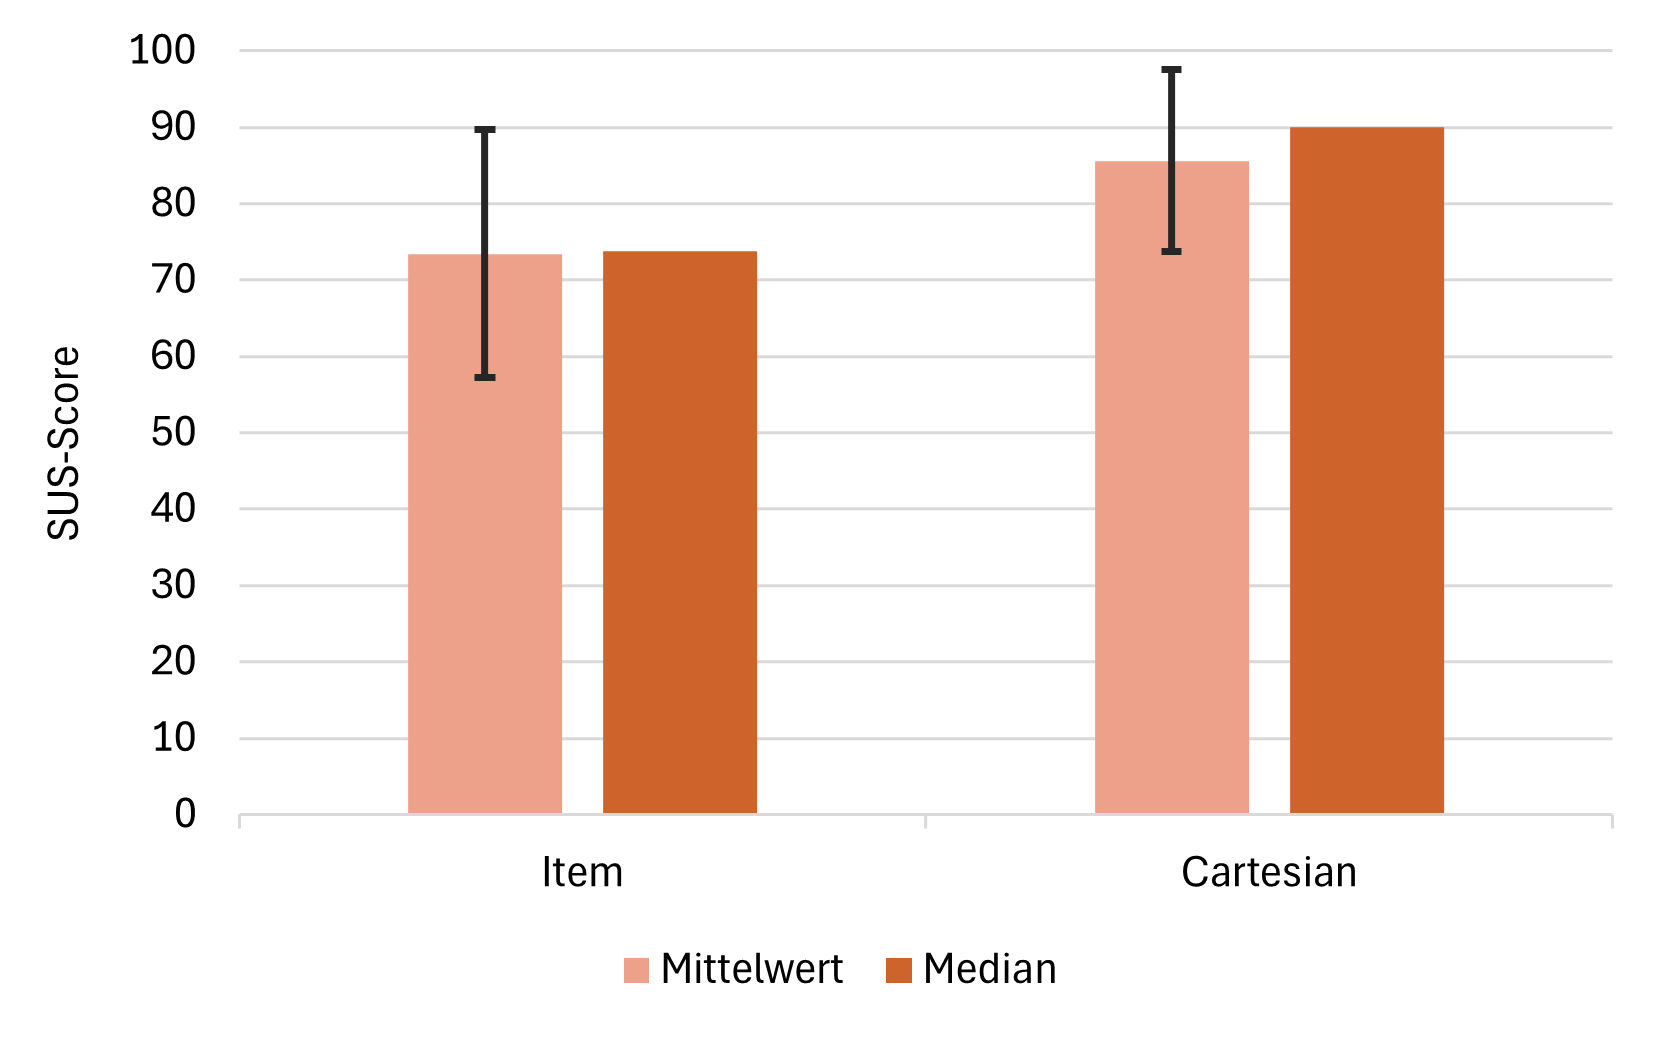
\includegraphics[scale=0.75]{images/Results/SUS-Scores.png}
    \caption{Mittelwerte und Median der SUS-Scores beider Verfahren}
    \label{fig:resultsSUS}
   \end{figure}

Die detaillierte Verteilung der Scores ist in \autoref{fig:histoSUS} dargestellt. Für das Item Scanning variieren die SUS-Scores zwischen 47,5 und 97,5. Der größte Anteil (drei Personen) liegt im Bereich 52,5-57,5. Insgesamt bewerteten 7 von 16 Teilnehmenden (43,75\%) das Verfahren mit einem Score von 80 oder höher. Für das Cartesian Scanning liegen die SUS-Scores zwischen 57,5 und 97,5. Der größte Anteil der Teilnehmenden (sechs Personen) bewertete das Verfahren mit einem Score im Bereich 92,5-97,5. Insgesamt haben 11 von 16 Teilnehmenden (68,75\%) das Verfahren mit einem SUS-Score von mindestens 80 bewertet. 

\begin{figure}
    \centering
    \begin{subfigure} {.5\textwidth}
        \centering
        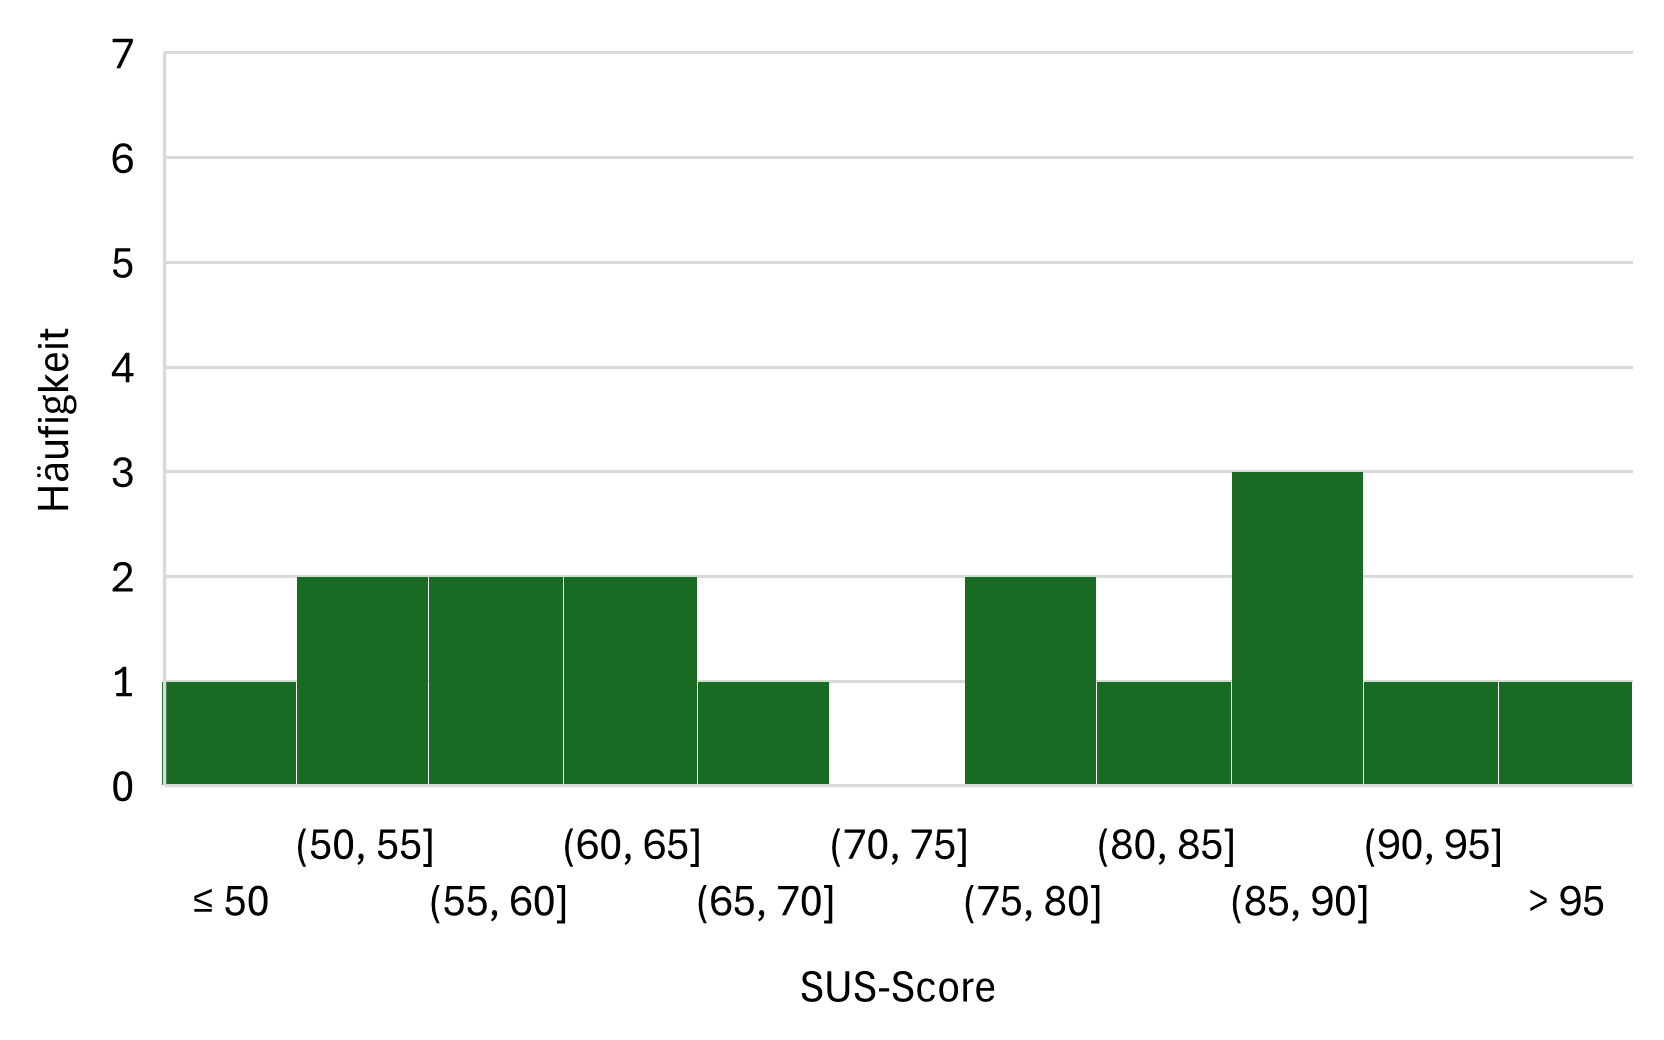
\includegraphics[width=.95\linewidth]{images/Results/Histogramm-SUS-Item.png}
        \caption{Item Scanning}
        \label{fig:histoSUSItem}
       \end{subfigure}%
       \begin{subfigure}{.5\textwidth}
        \centering
       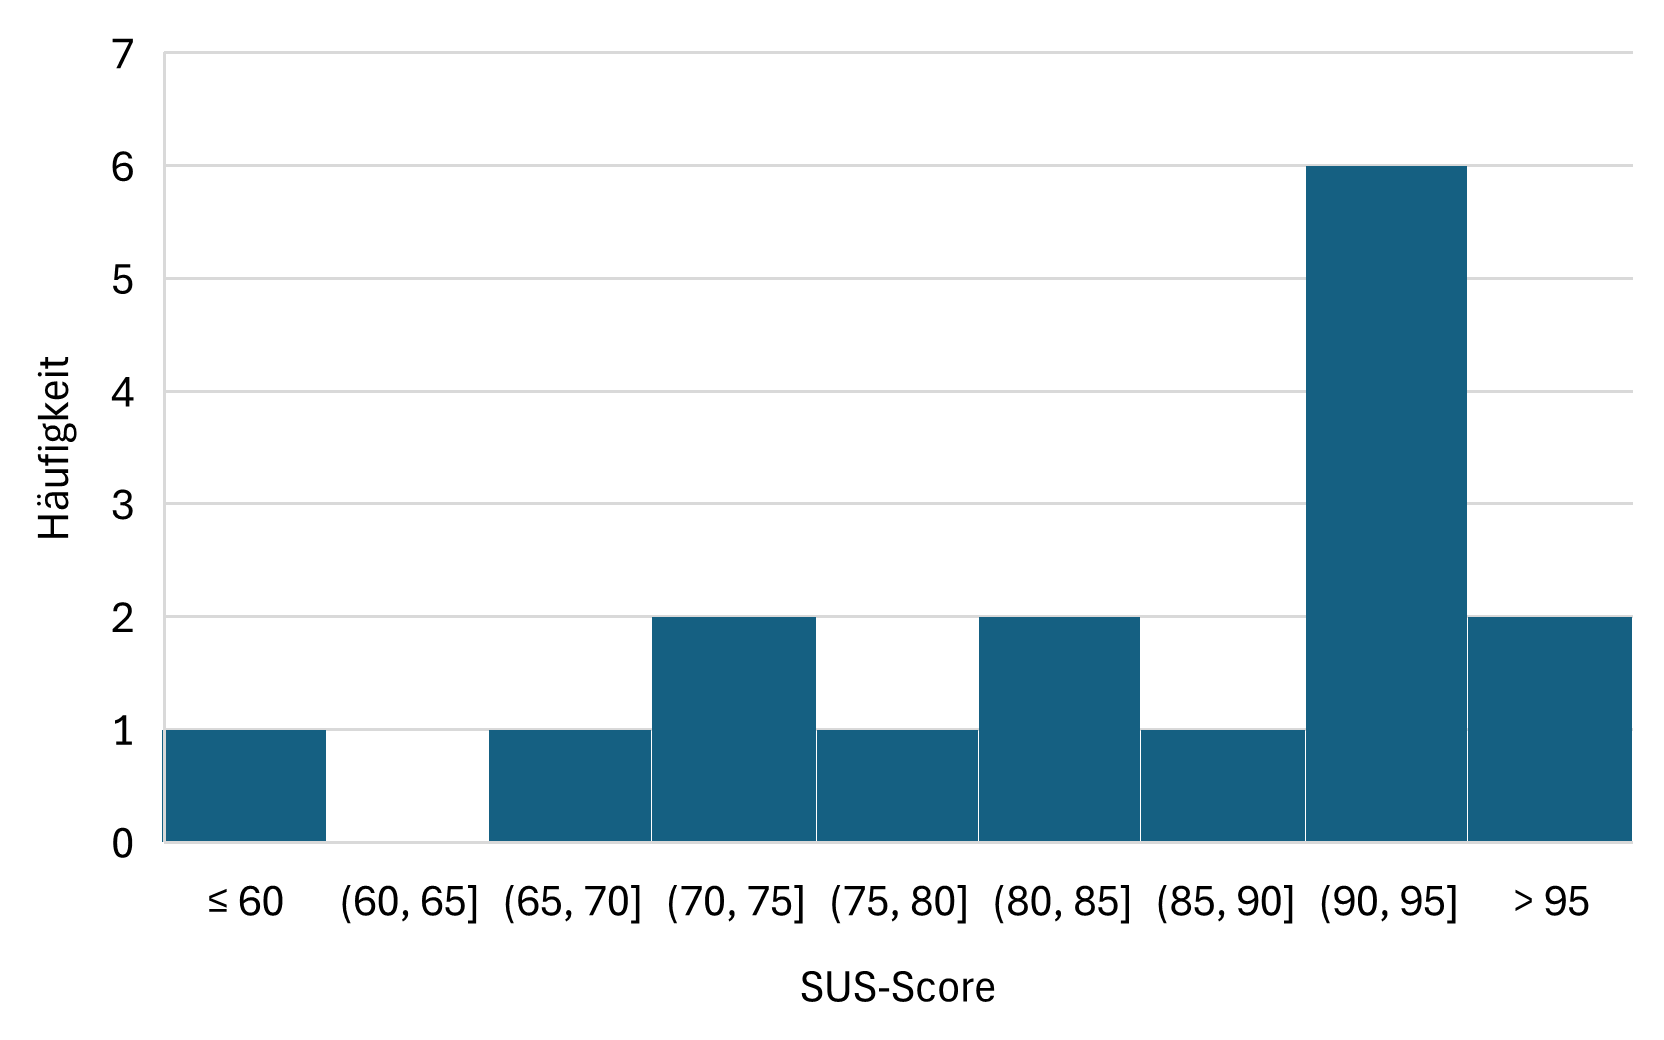
\includegraphics[width=.98\linewidth]{images/Results/Histogramm-SUS-Cartesian.png}
        \caption{Cartesian Scanning}
        \label{fig:histoSUSCartesian}
       \end{subfigure}
       \caption{Verteilung der SUS Scores beider Verfahren}
       \label{fig:histoSUS}
\end{figure}


Die Ergebnisse des User Experience Questionnaire (UEQ) wurden mit Hilfe des Auswertungstools der Autoren analysiert. Für jeden der sechs Faktoren wurden Mittelwerte und Varianzen berechnet. Die \autoref{fig:ueqScalesItem} zeigt die berechneten Mittelwerte und Varianzen für das Item Scanning. In \autoref{fig:ueqScoreItem} werden diese Ergebnisse zusätzlich visualisiert. 

\begin{figure}[tbh]
    \centering
   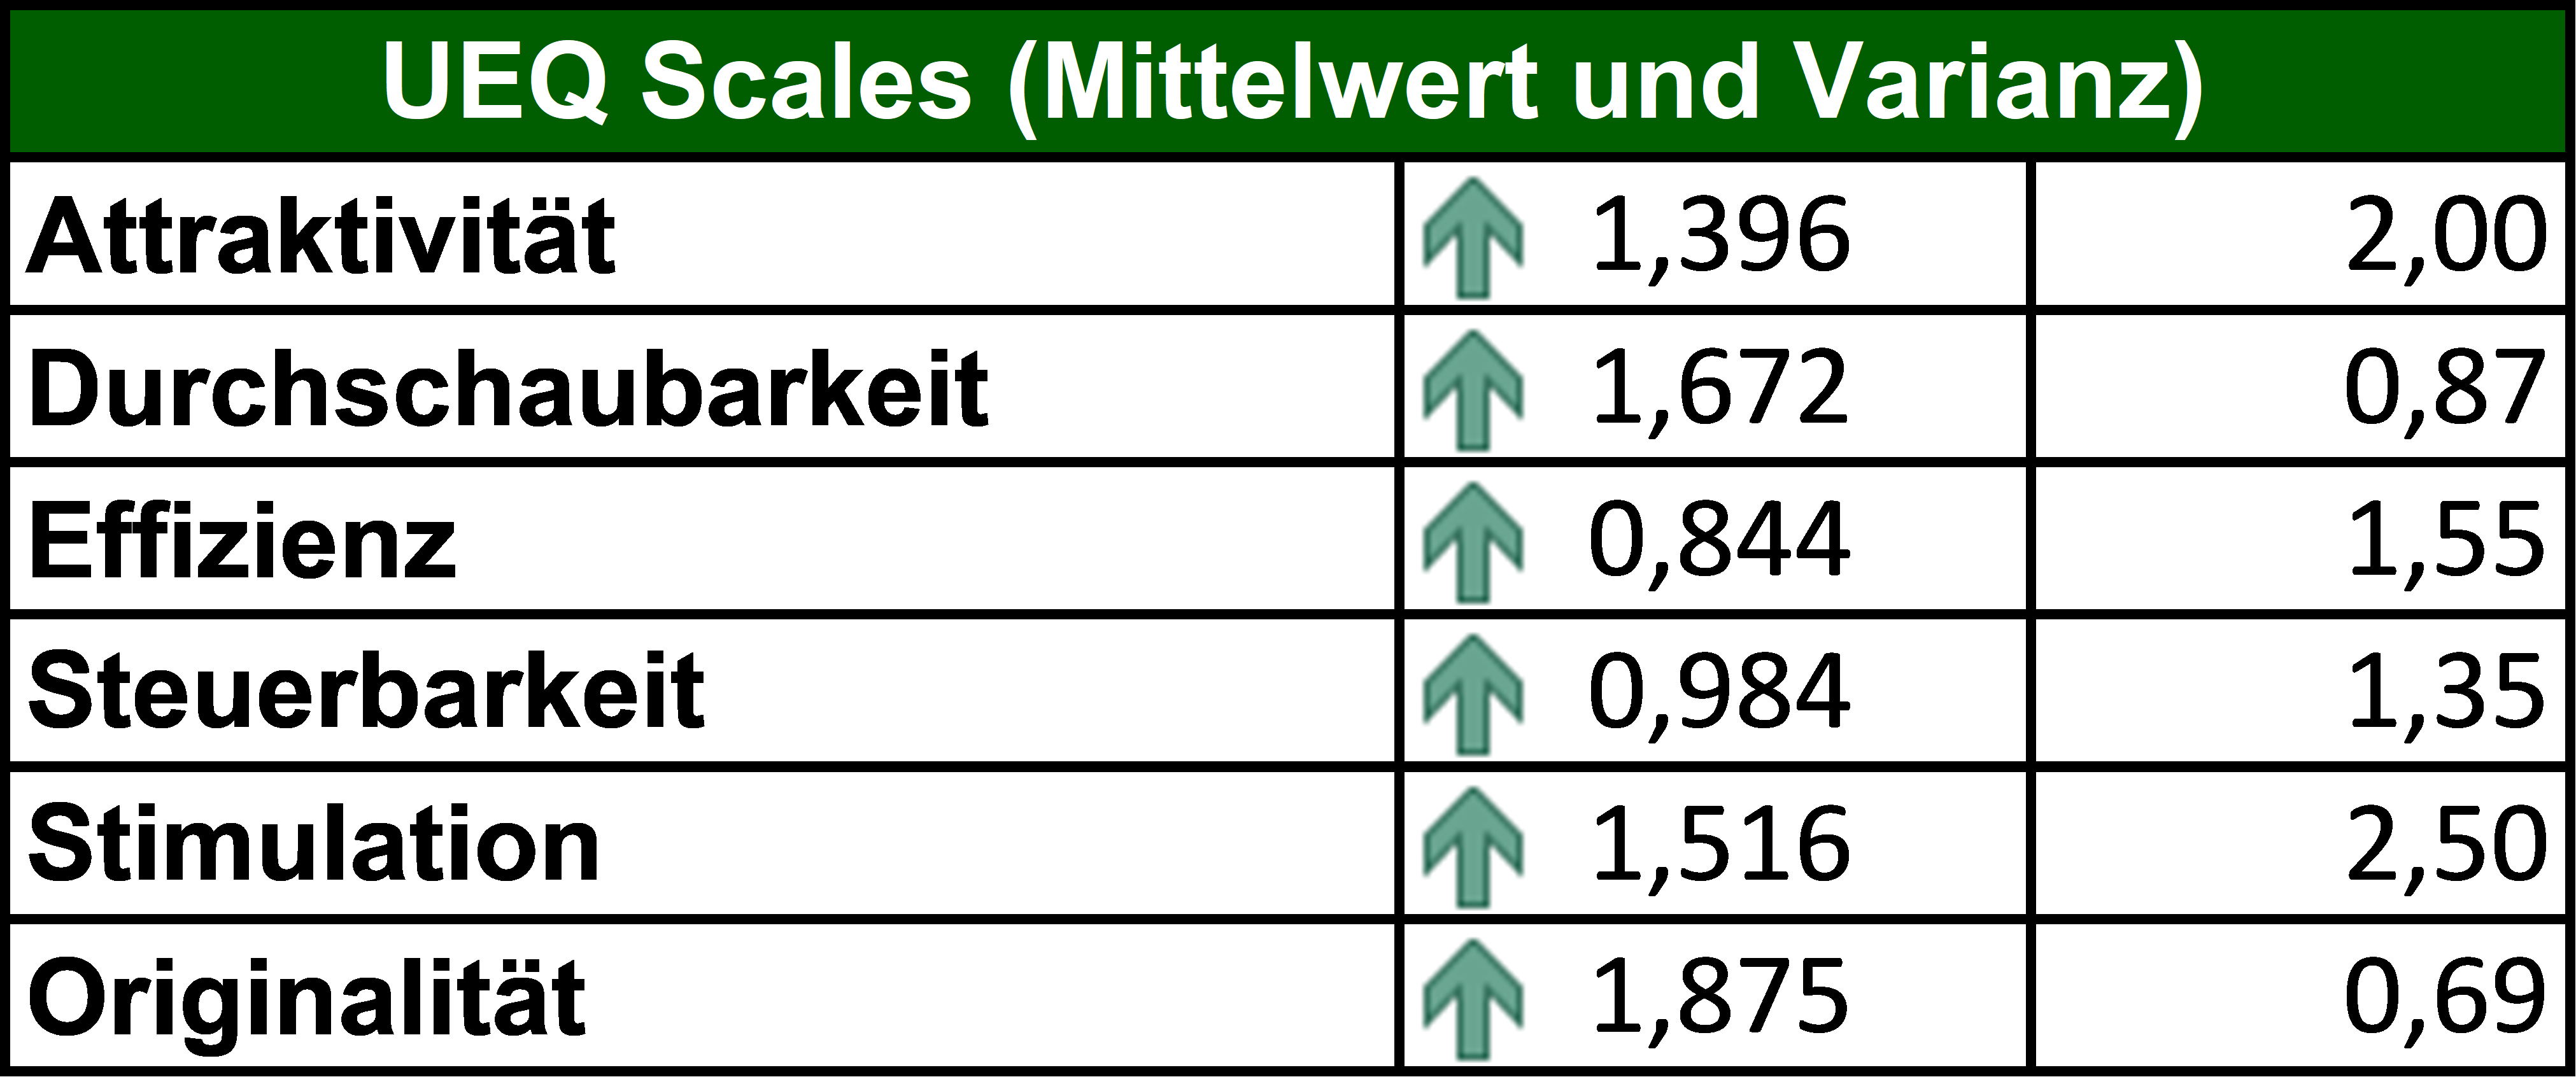
\includegraphics{images/Results/UEQ-Table-Means-Item.png}
    \caption{Ergebnisse UEQ Item Scanning}
    \label{fig:ueqScalesItem}
   \end{figure}

\begin{figure}[tbh]
    \centering
   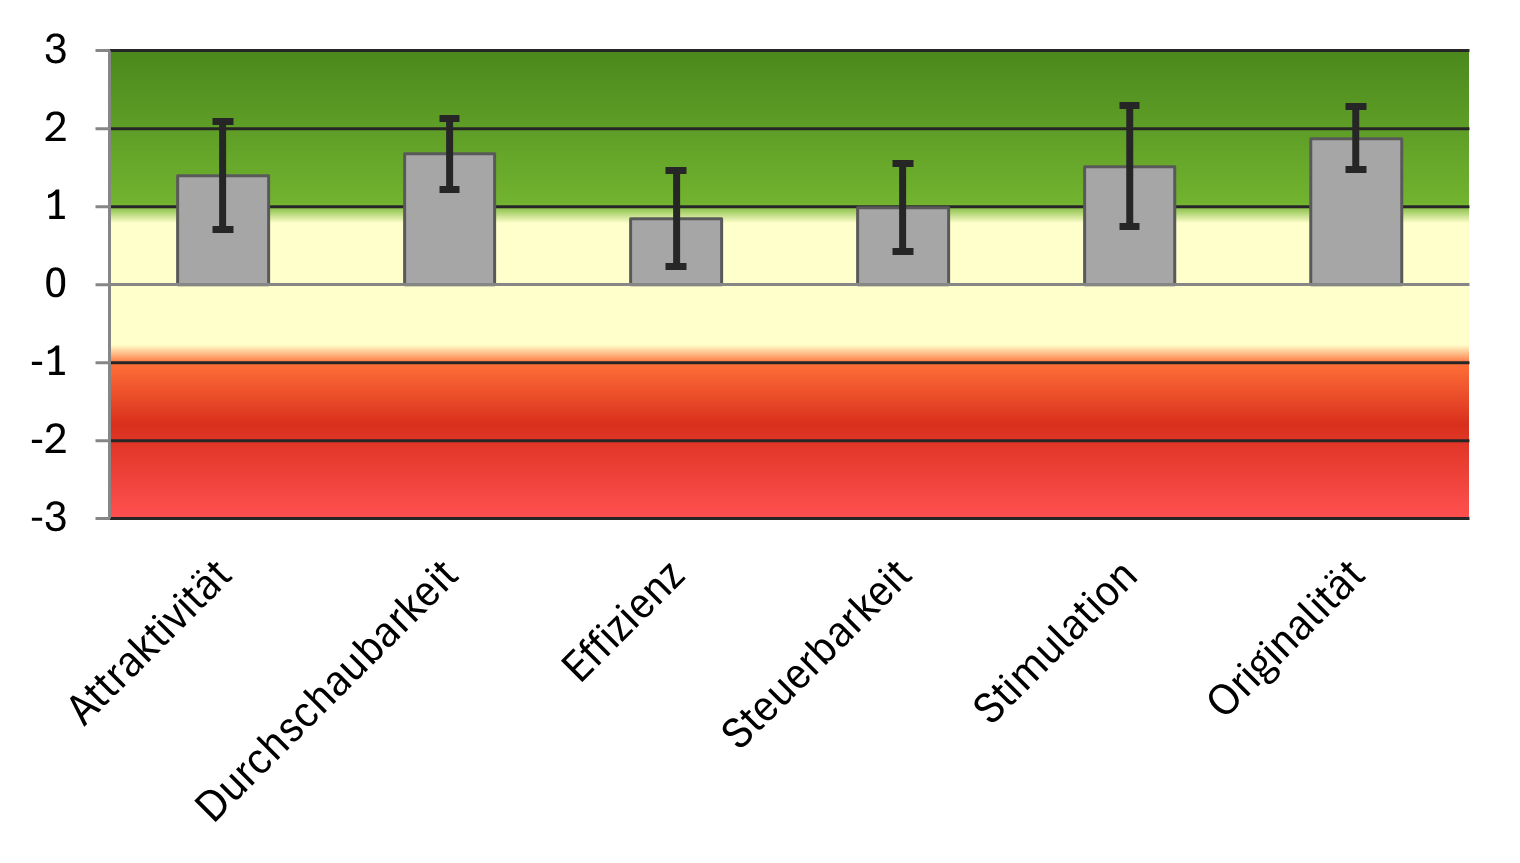
\includegraphics{images/Results/UEQ-Item.png}
    \caption{Ergebnisse UEQ Item Scanning}
    \label{fig:ueqScoreItem}
   \end{figure}


Für das Item Scanning liegen die Mittelwerte der Bewertungen im positiven Bereich. Den höchsten Wert weist der Faktor Originalität mit einem Mittelwert von 1,875 bei einer Varianz von 0,69 auf, gefolgt von Durchschaubarkeit (Mittelwert: 1,672, Varianz: 0,87) und Stimulation (Mittelwert: 1,516, Varianz: 2,50). Am niedrigsten wurden die Faktoren Steuerbarkeit und Effizienz bewertet. Hier liegen die Mittelwerte bei 0,984 und 0,844 mit Varianzen von 1,35 und 1,55. 

Die Ergebnisse für das Cartesian Scanning sind in \autoref{fig:ueqScalesCartesian} dargestellt und in \autoref{fig:ueqScoreCartesian} visualisiert. 

Das Cartesian Scanning wurde insgesamt besser bewertet als das Item Scanning. Der Faktor Durchschaubarkeit wurde mit einem Mittelwert von 2,234 und einer Varianz von 0,53 am höchsten bewertet. Die Faktoren Attraktivität, Stimulation und Originalität wurden mit Mittelwerten von 1,833, 1,734 und 1,750 ähnlich hoch bewertet. Den niedrigsten Mittelwert und gleichzeitig die höchste Varianz weist der Faktor Effizienz auf. Hier liegt der Mittelwert bei 1,063 bei einer Varianz von 1,33. 

\begin{figure}[tbh]
    \centering
   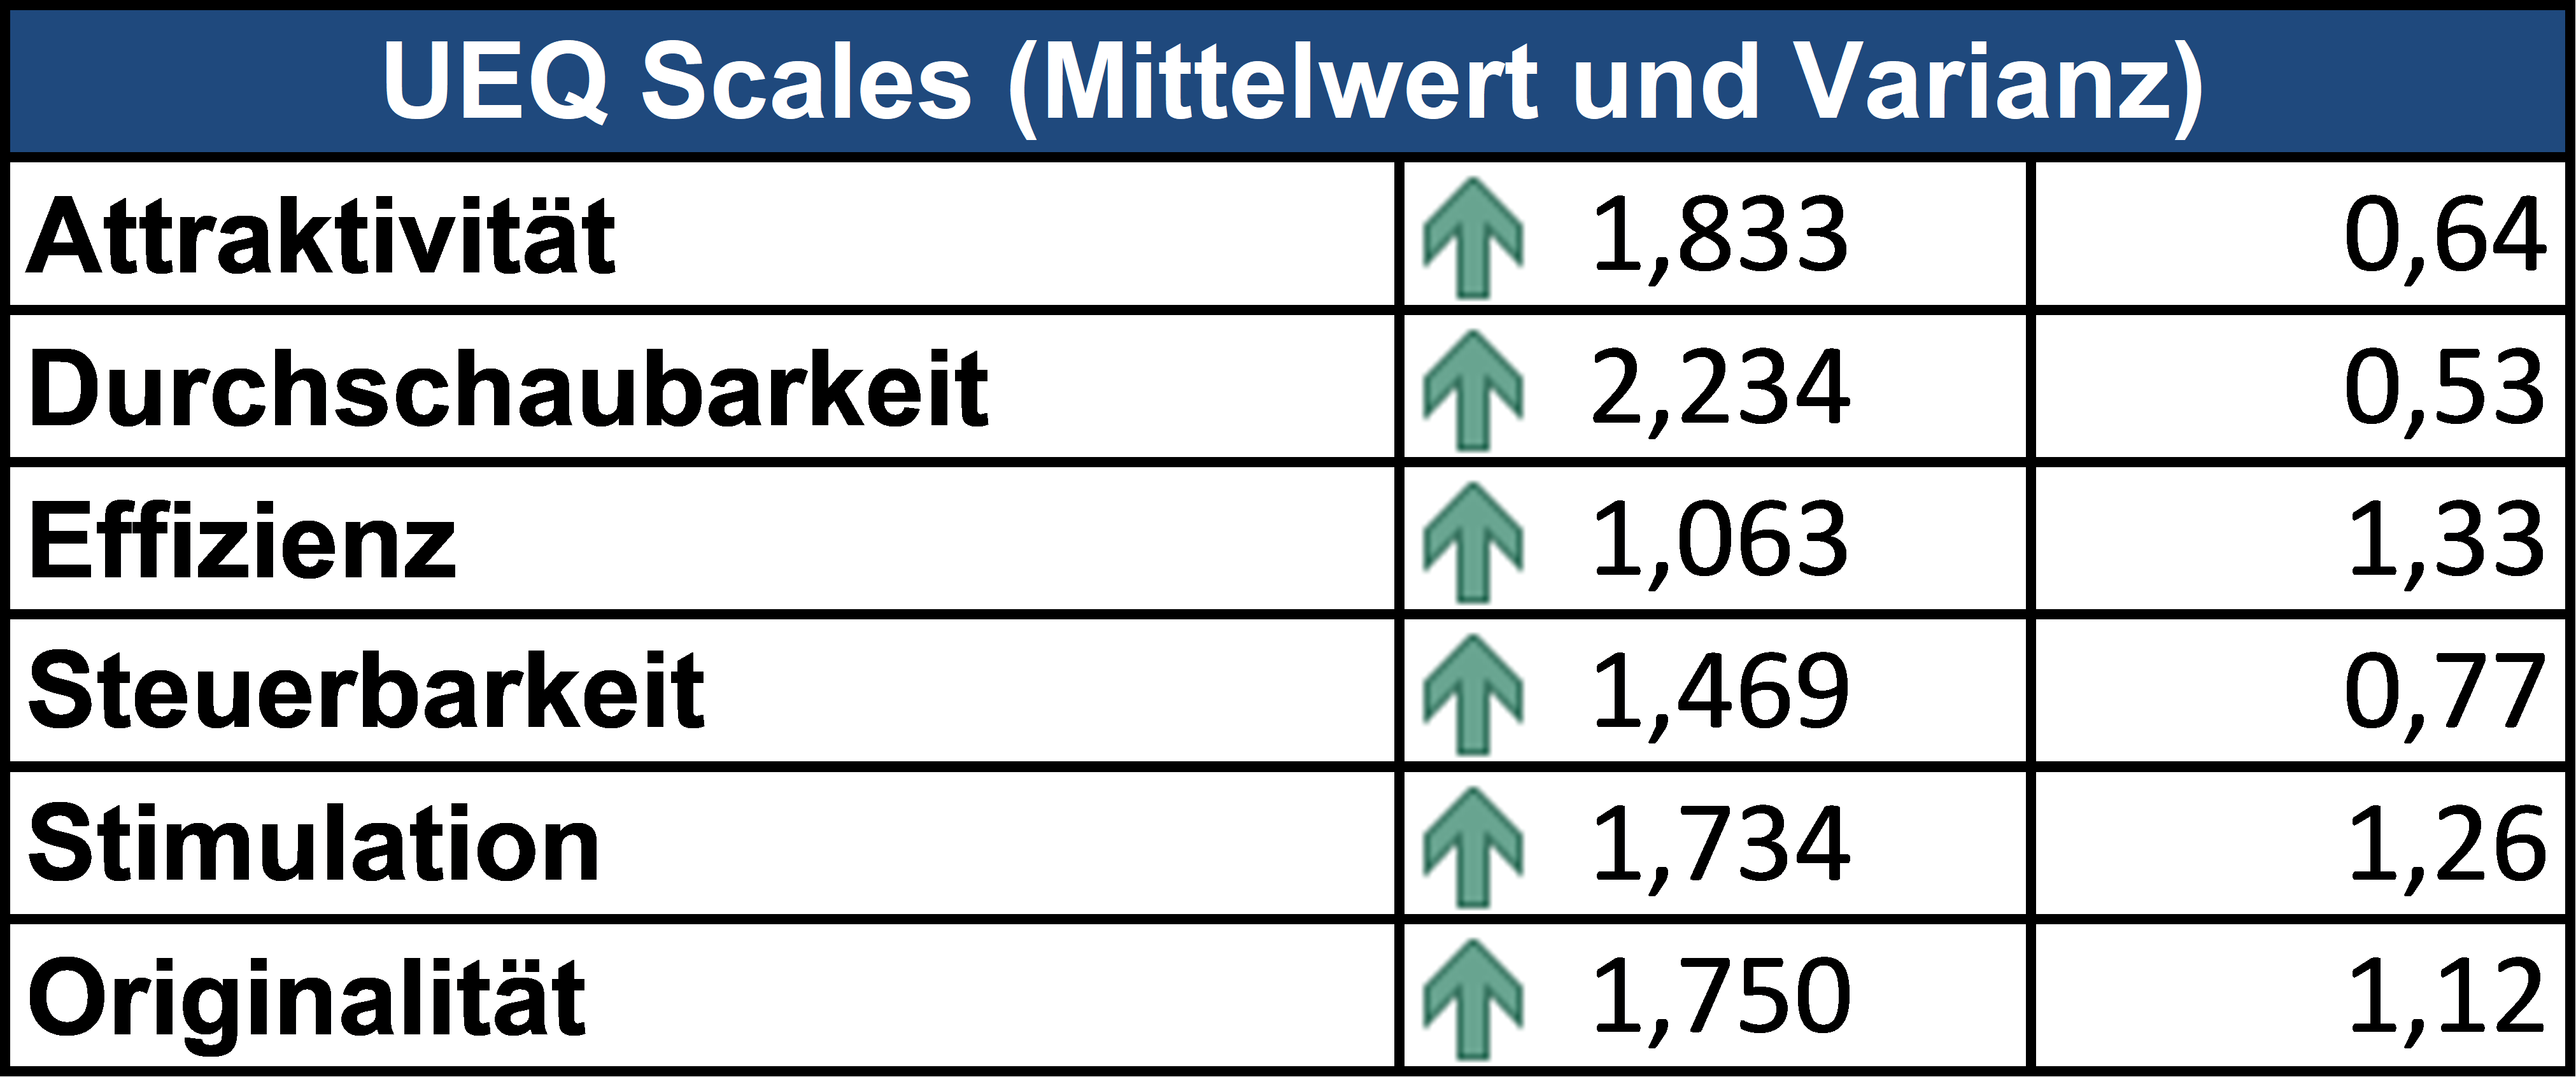
\includegraphics{images/Results/UEQ-Table-Means-Cartesian.png}
    \caption{Ergebnisse UEQ Cartesian Scanning}
    \label{fig:ueqScalesCartesian}
   \end{figure}

\begin{figure}[tbh]
 \centering
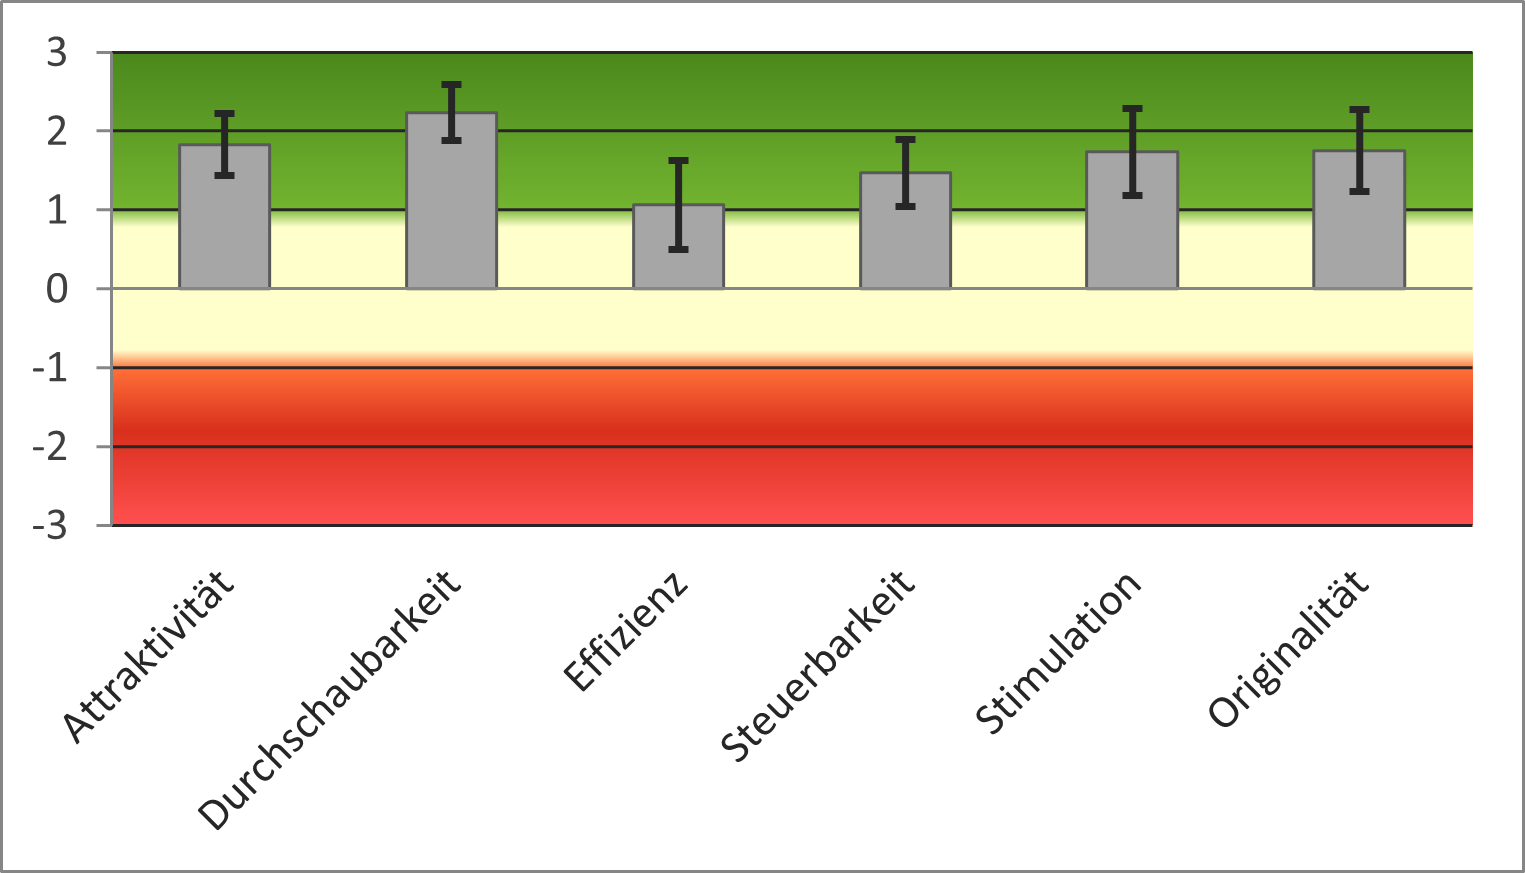
\includegraphics{images/Results/UEQ-Cartesian.png}
 \caption{Ergebnisse UEQ Cartesian Scanning}
 \label{fig:ueqScoreCartesian}
\end{figure}


\subsection{Motion Sickness (SSQ)} 

Die Ergebnisse des Simulator Sickness Questionnaire (SSQ) werden in \autoref{fig:tableSymptomsSSQ} dargestellt. Die Tabelle zeigt die im Fragebogen erfassten Symptome sowie die jeweilige Symptomkategorie (N: Nausea, O: Oculomotor, D: Disorientation). Für beide Verfahren wird für jedes Symptom die Häufigkeit angegeben, mit der es auftrat. Dies entspricht der Anzahl der Personen, die einen Wert >0 angaben. Zusätzlich wird in einer weiteren Spalte dargestellt, wie viele dieser Personen in der Auswertung jeweils einen Wert >1 angegeben haben und somit eine moderate bis starke Ausprägung des Symptoms empfunden haben. 
Es zeigt sich, dass beim Item Scanning die Symptome angestrengte Augen (11 Personen, davon 4 mit moderater Ausprägung) sowie Ermüdung, Kopfdruck und verschwommenes Sehen (6 Personen, keine moderaten Ausprägungen) am häufigsten auftraten. Vereinzelt wurde von allgemeinem Unwohlsein, Konzentrationsschwierigkeiten, Schwitzen, erhöhtem Speichelfluss, Schwindel und Übelkeit berichtet, wobei diese Symptome jeweils nur eine oder zwei Personen betrafen und nur in leichter Ausprägung auftraten. Symptome wie Aufstoßen oder Gleichgewichtsstörungen wurden nicht genannt.
Beim Cartesian Scanning ergab sich eine ähnliche Verteilung. Am häufigsten wurden angestrengte Augen (11 Personen, davon 2 mit moderater Ausprägung) und Ermüdung (8 Personen, keine moderaten Ausprägungen) berichtet. Im Vergleich zum Item Scanning traten verschwommenes Sehen und Kopfdruck etwas seltener auf (3 bzw. 4 Personen). Weitere Symptome wie Konzentrationsschwierigkeiten oder Schwitzen traten ebenfalls nur vereinzelt auf, während allgemeines Unwohlsein, Übelkeit und Gleichgewichtsstörungen nicht aufgetreten sind.

\begin{figure}[tbh]
    \centering
    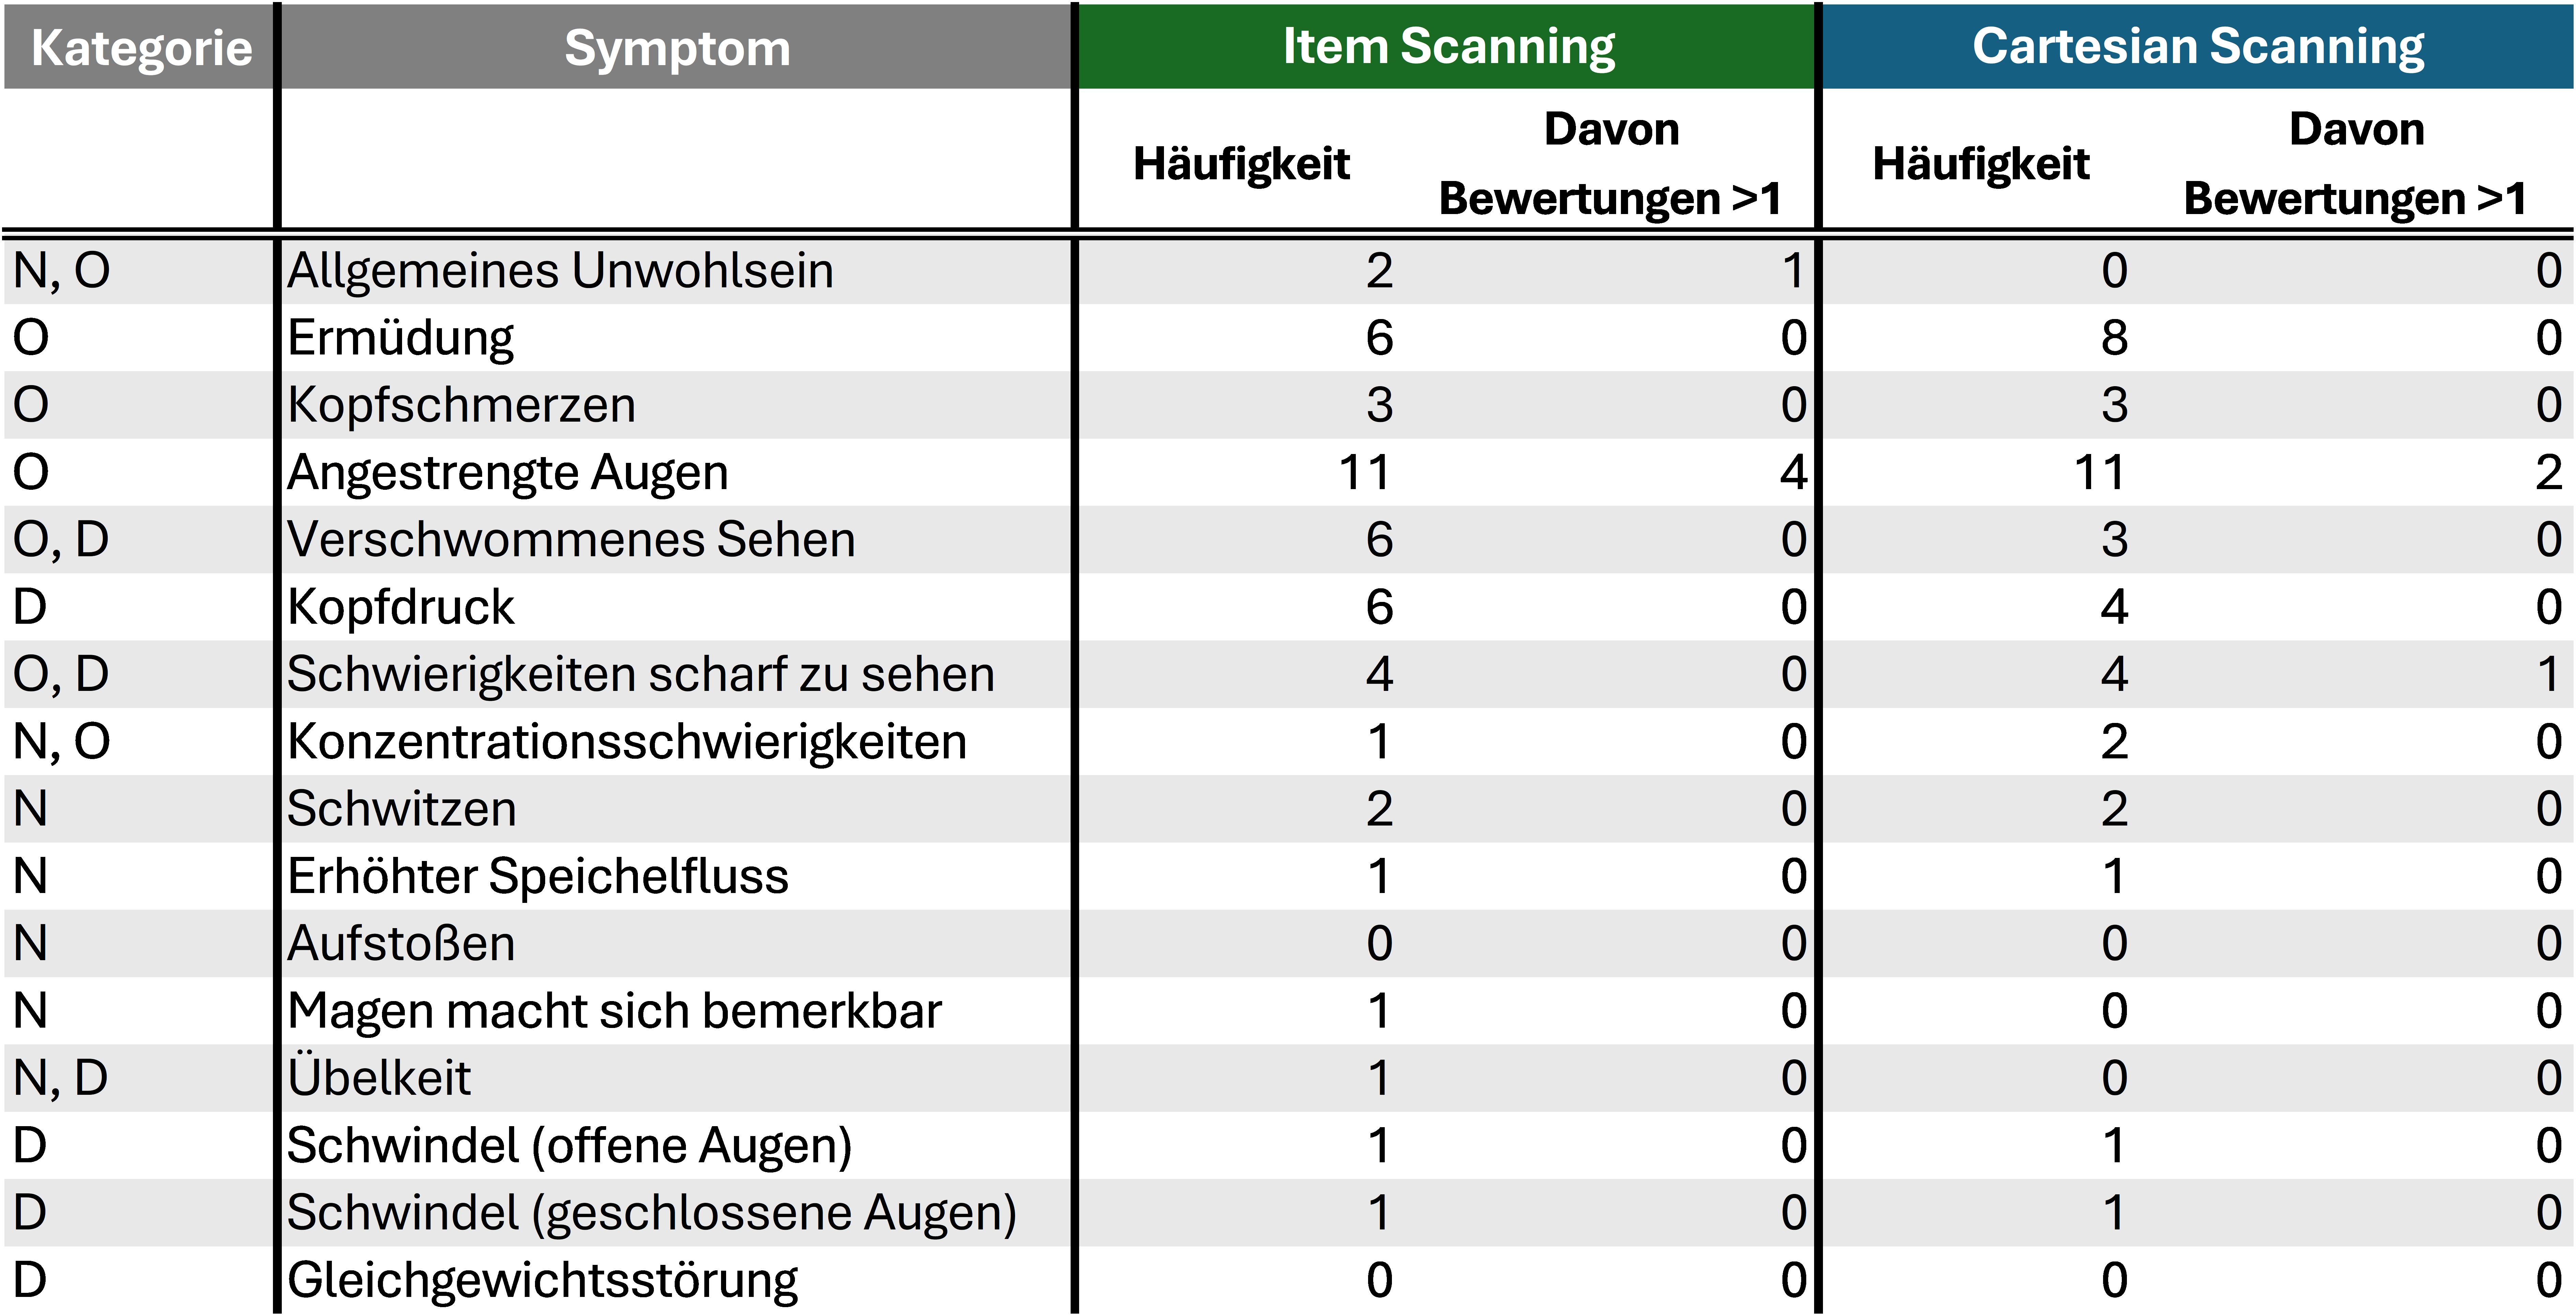
\includegraphics[width=0.95\textwidth]{images/Results/SSQ-Table-2.png}
    \caption{Häufigkeit der SSQ-Symptome beider Verfahren }
    \label{fig:tableSymptomsSSQ}
\end{figure}

Die weitere Auswertung des SSQ erfolgte nach der Beschreibung der Autoren \citep{kennedy_simulator_1993}. Dazu wurden zunächst die gewichteten Scores der einzelnen Kategorien und anschließend der Gesamtscore bestimmt. Die Ergebnisse sind in \autoref{fig:tableErgebnisseSSQ} dargestellt. Die Verteilung der Gesamtscores ist darüber hinaus in \autoref{fig:histoSSQScore} visualisiert. 

\begin{figure}[tbh]
    \centering
    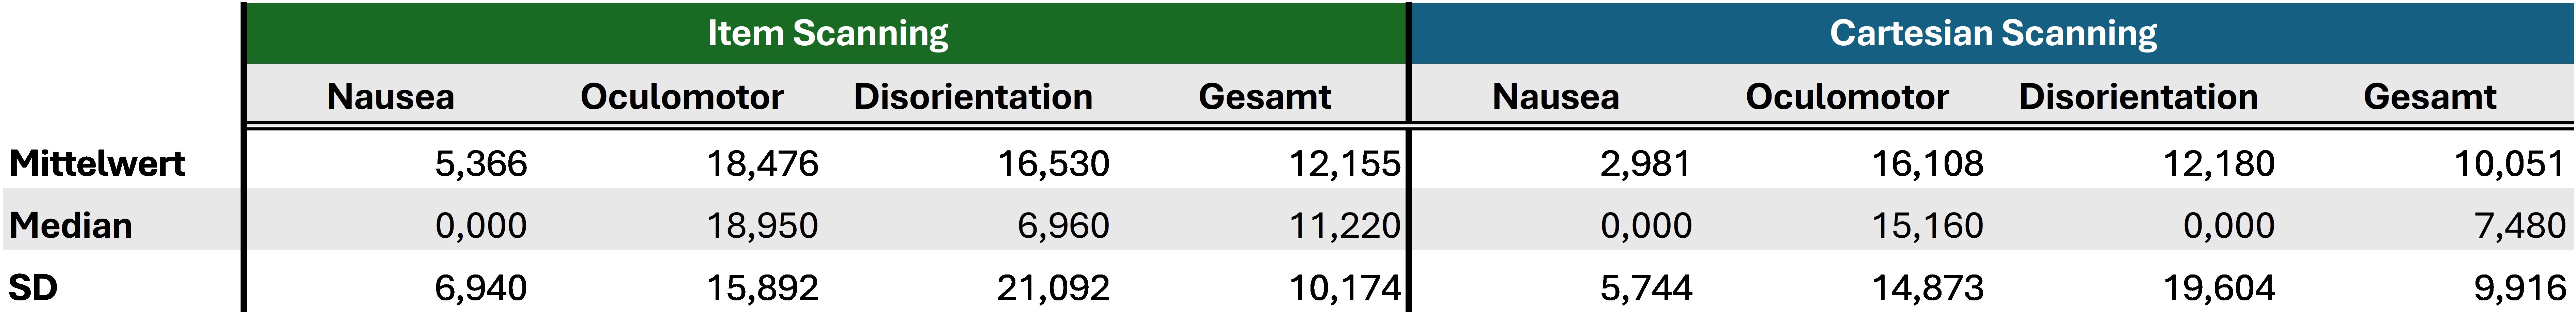
\includegraphics[width=0.95\textwidth]{images/Results/Tabelle-Ergebnisse-SSQ.png}
    \caption{Mittelwerte der Ergebnisse des SSQ nach Verfahren und Kategorie}
    \label{fig:tableErgebnisseSSQ}
\end{figure}

\begin{figure}
    \centering
    \begin{subfigure}{.5\textwidth}
        \centering
        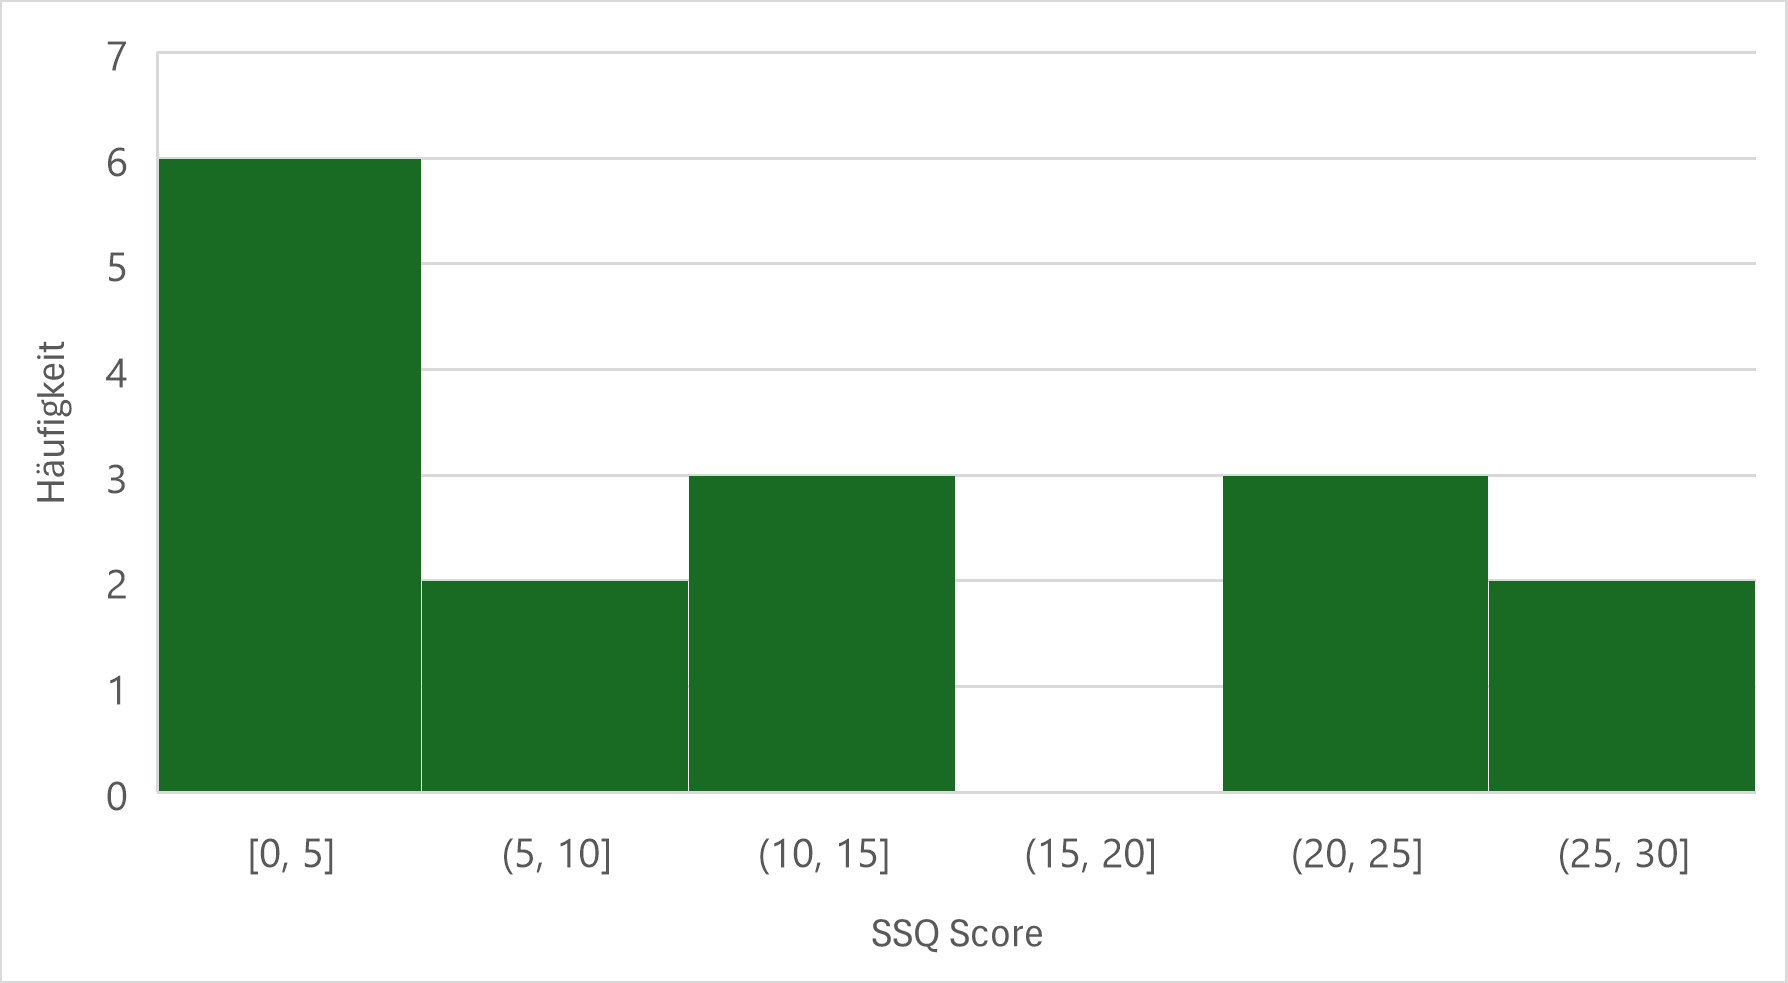
\includegraphics[width=0.99\textwidth]{images/Results/Histogramm-SSQScores-Item.png}
        \caption{Item Scanning}
        \label{fig:histoSSQItem}   
    \end{subfigure}%
    \begin{subfigure}{.5\textwidth}
        \centering
        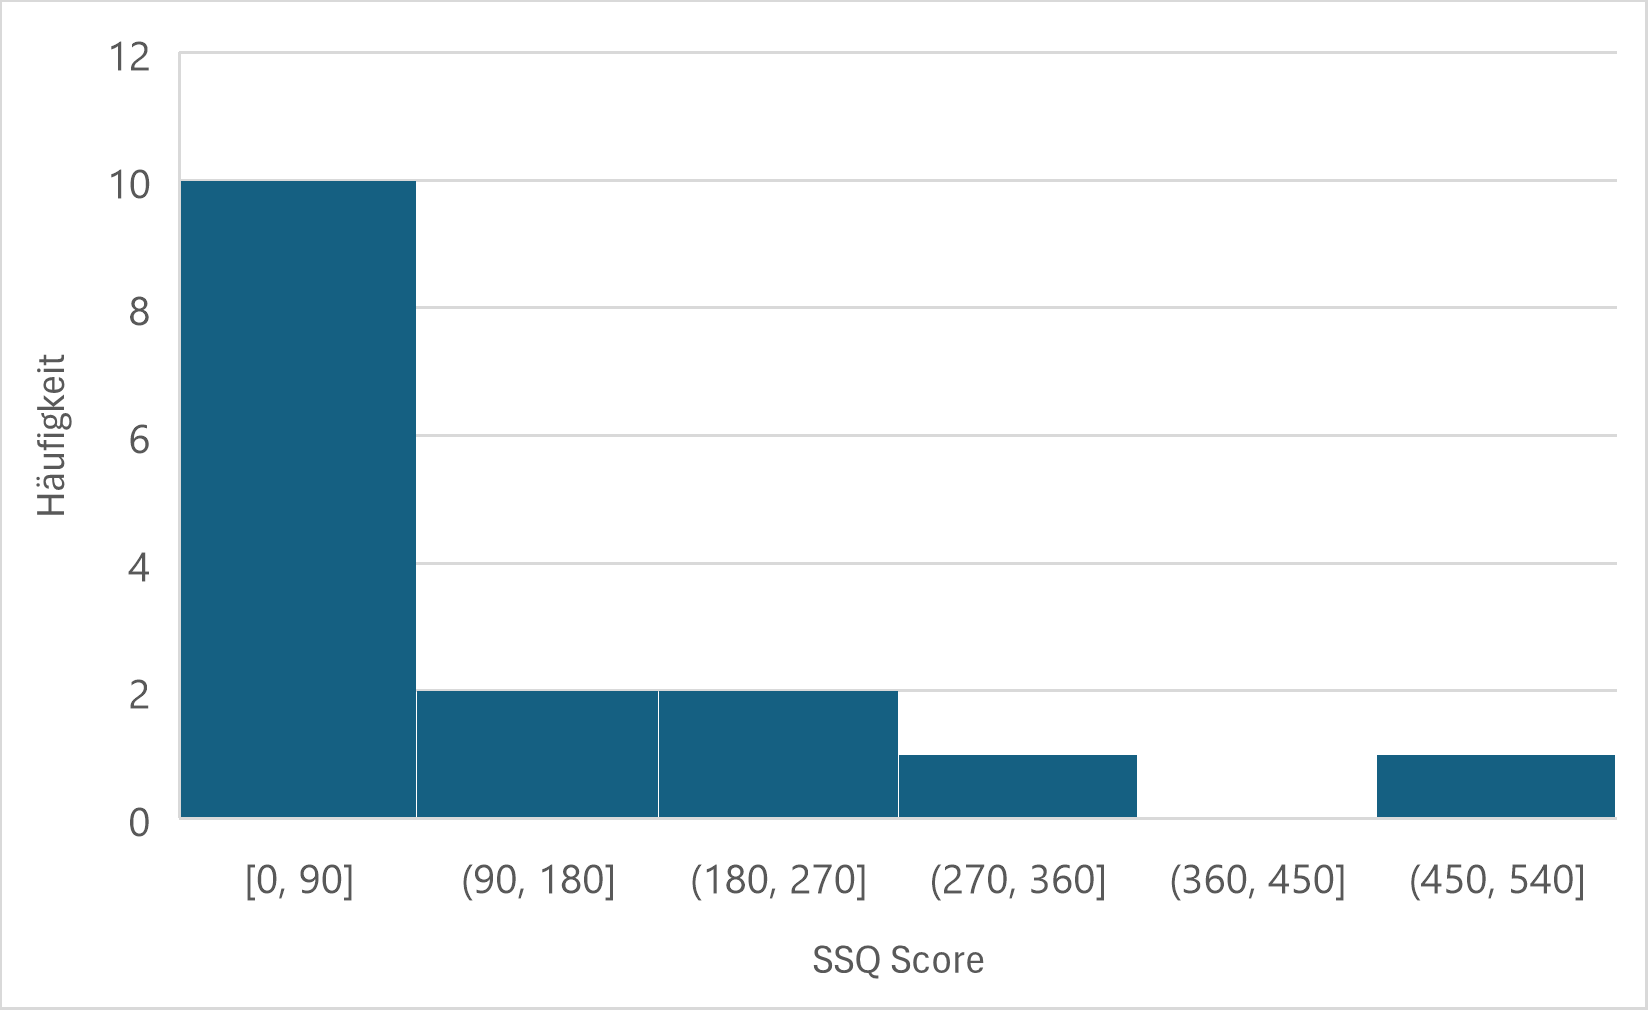
\includegraphics[width=0.99\textwidth]{images/Results/Histogramm-SSQScores-Cartesian.png}
         \caption{Cartesian Scanning}
         \label{fig:histoSSQCartesian}
    \end{subfigure}
    \caption{Verteilung der SSQ-Scores beider Verfahren}
    \label{fig:histoSSQScore}
\end{figure}

Die Histogramme zeigen, dass die meisten Teilnehmenden bei beiden Verfahren einen SSQ-Wert zwischen 0 und 5 aufwiesen (jeweils 6 Personen). Beim Cartesian Scanning liegt der höchste Score bei 37,40 und damit deutlich höher als beim Item Scanning (29,92). Allerdings erreichten beim Item Scanning insgesamt mehr Personen einen Score größer 10 (8 Personen gegenüber 6 Personen). Der Mittelwert des Gesamtscores liegt beim Item Scanning bei 12,155 (Standardabweichung: 10,174) und beim Cartesain Scanning bei 10,051 (Standardabweichung: 9,916) (vgl. \autoref{fig:tableErgebnisseSSQ}).

Um genauere Aussagen darüber treffen zu können, in welchen Kategorien die meisten Symptome auftraten, werden die Ergebnisse der Scores der Kategorien folgend genauer betrachtet.

\begin{figure}
    \centering
    \begin{subfigure}{.5\textwidth}
        \centering
        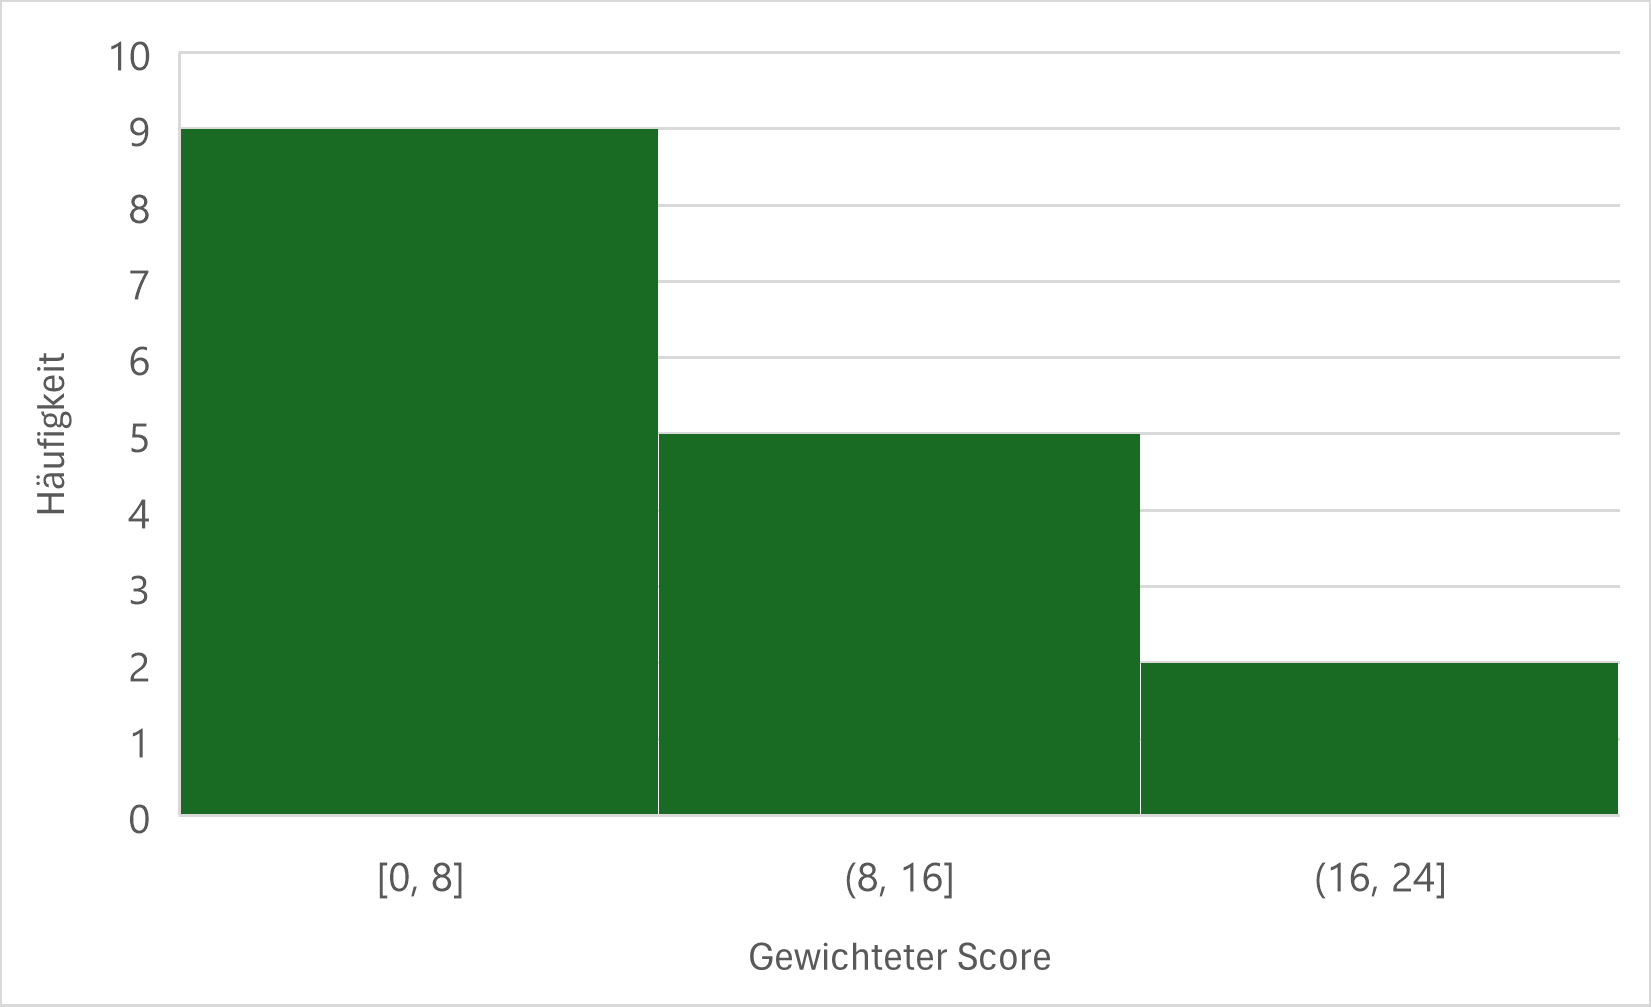
\includegraphics[width=0.99\textwidth]{images/Results/Histogramm-Nausea-Scale-Item.png}
        \caption{Item Scanning}
        \label{fig:histoNauseaItem}   
    \end{subfigure}%
    \begin{subfigure}{.5\textwidth}
        \centering
        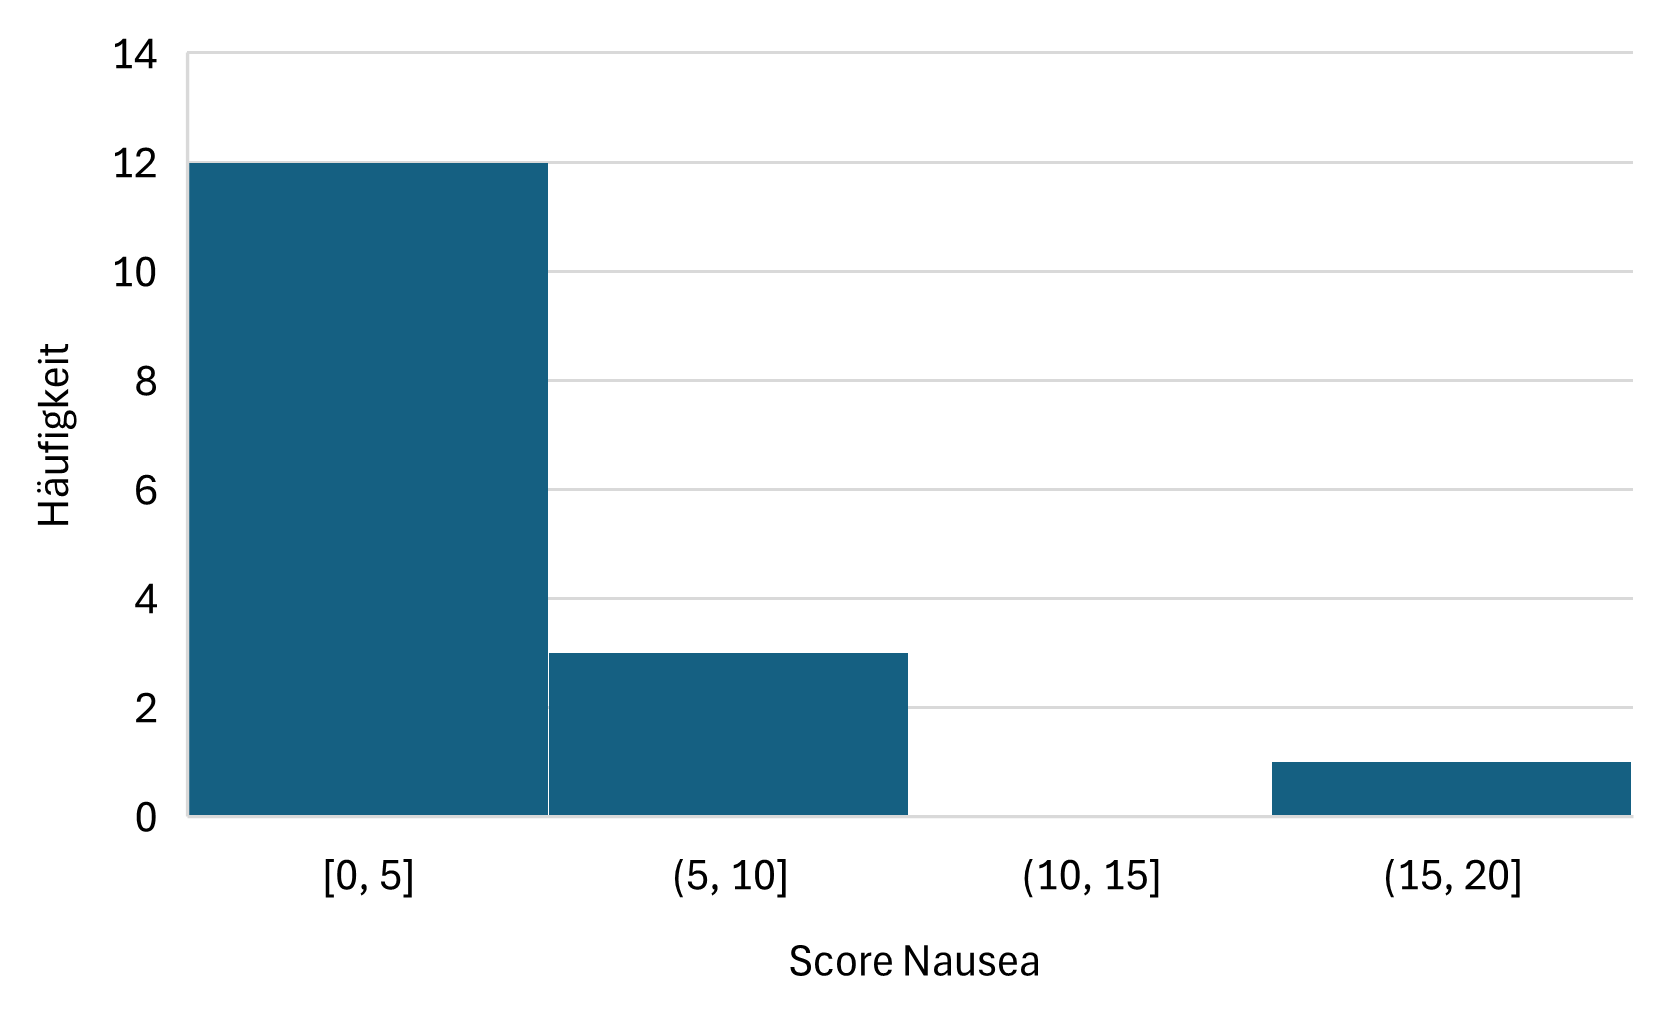
\includegraphics[width=0.99\textwidth]{images/Results/Histogramm-Nausea-Scale-Cartesian.png}
         \caption{Cartesian Scanning}
         \label{fig:histoNauseaCartesian}
    \end{subfigure}
    \caption{Verteilung der Scores der SSQ Nausea Scale beider Verfahren}
    \label{fig:histoNausea}
\end{figure}

In der Kategorie Nausea (vgl. \autoref{fig:histoNausea}) berichteten beim Item Scanning neun Personen keine Symptome. Fünf Teilnehmende zeigten Scores zwischen 8 und 10, was dem Auftreten eines einzigen Symptoms in leichter Ausprägung entspricht. Zwei Personen erreichten Scores über 15, was dem Auftreten mehrerer Symptome oder mindestens einem Symptom in moderater bis starker Ausprägung entspricht. Der Mittelwert der Scores dieser Kategorie liegt bei 5,366 (Standardabweichung: 6,940) (vgl. \autoref{fig:tableErgebnisseSSQ}). Beim Cartesian Scanning hingegen zeigten zwölf Personen keine Symptome. Drei Personen erreichten einen Score zwischen 5 und 10 und eine Person einen Score über 15. Der Mittelwert für das Cartesian Scanning in dieser Kategorie liegt bei 2,981 (Standardabweichung: 5,744) (vgl. \autoref{fig:tableErgebnisseSSQ}).

\begin{figure}
    \centering
    \begin{subfigure}{.5\textwidth}
        \centering
        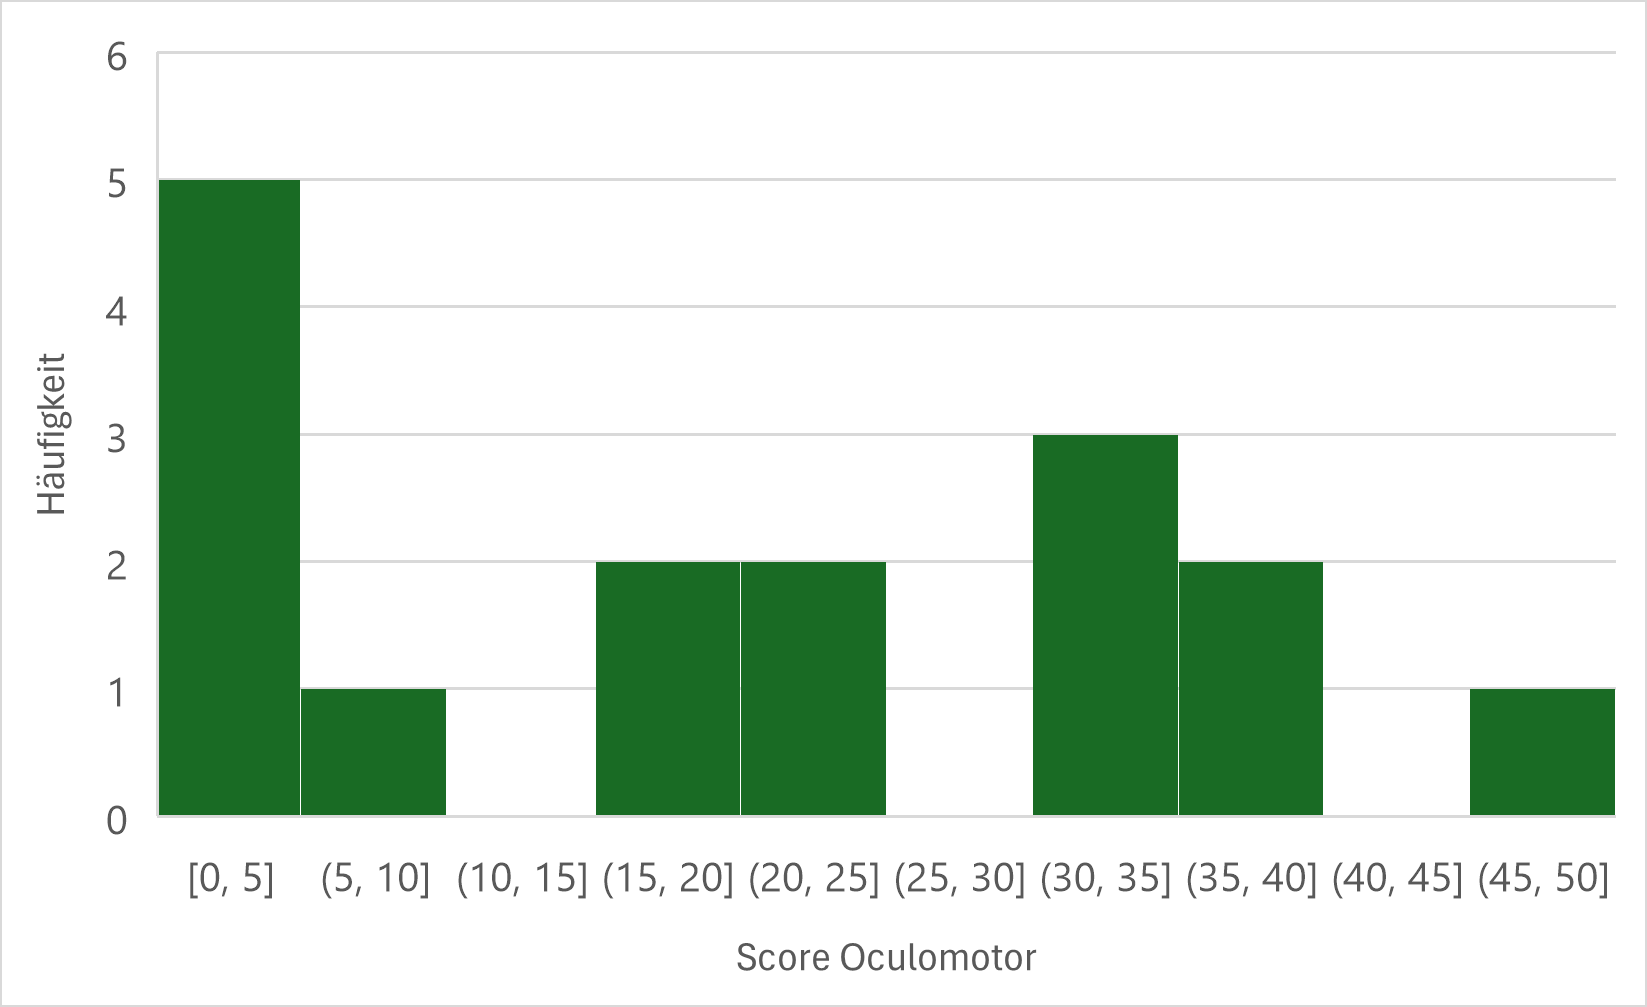
\includegraphics[width=0.99\textwidth]{images/Results/Histogramm-Oculomotor-Scale-Item.png}
        \caption{Item Scanning}
        \label{fig:histoOculomotorItem}   
    \end{subfigure}%
    \begin{subfigure}{.5\textwidth}
        \centering
        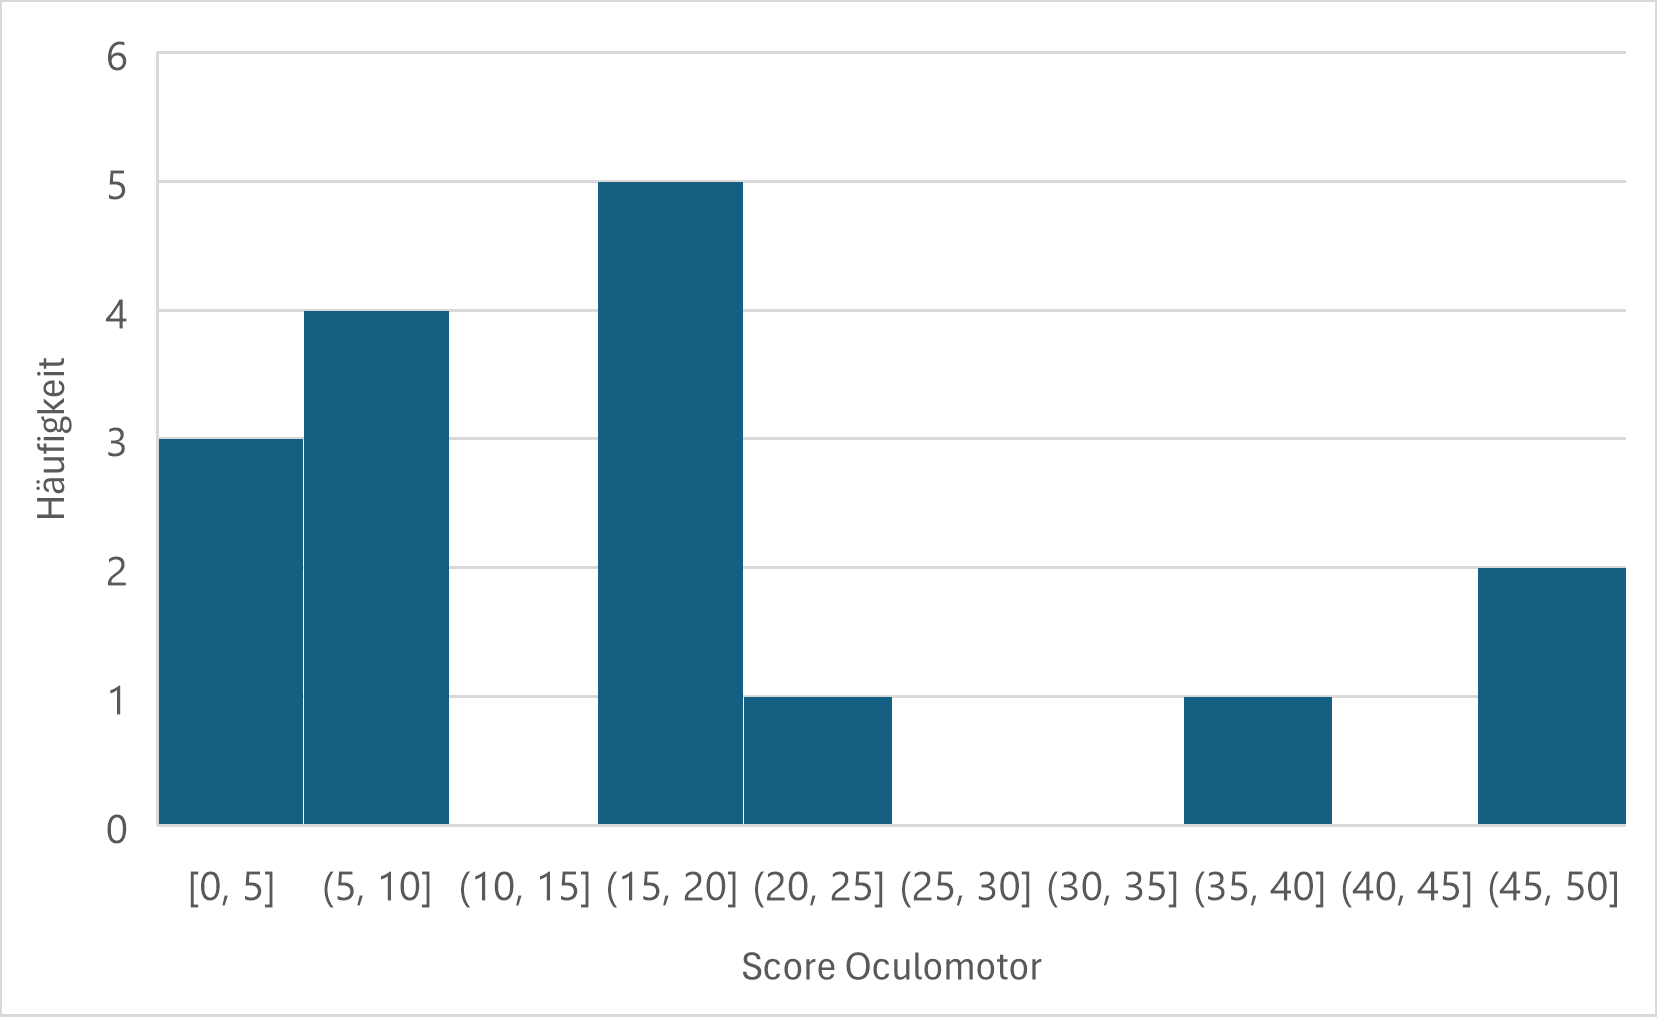
\includegraphics[width=0.99\textwidth]{images/Results/Histogramm-Oculomotor-Scale-Cartesian.png}
         \caption{Cartesian Scanning}
         \label{fig:histoOculomotorCartesian}
    \end{subfigure}
    \caption{Verteilung der Scores der SSQ Oculomotor Scale beider Verfahren}
    \label{fig:histoOculomotor}
\end{figure}

In der Kategorie Oculomotor (vgl. \autoref{fig:histoOculomotor}) traten häufiger Symptome auf. Während beim Item Scanning sechs Personen keine bis nur sehr leichte Symptome (Score <10) aufwiesen, erreichten sieben Teilnehmende einen Score zwischen 15 und 35. Dies entspricht dem auftreten von zwei oder mehr leichten oder mindestens einem moderaten Symptom. Drei Teilnehmende erreichten einen Score über 35, was auf das Auftreten mehrerer Symptome und mindestens einem Symptom in moderater Ausprägung hinwiest. Der Mittelwert der Scores dieser Kategorie liegt bei 18,476 (Standardabweichung: 15,892) (vgl. \autoref{fig:tableErgebnisseSSQ}). Beim Cartesian Scanning zeigten sieben Personen keine bis leichte Symptome. Fünf Personen wiesen einen Score zwischen 15 und 20 auf. Vier Personen erreichten einen Score größer 20, wobei zwei Personen einen Score von über 45 erreichten. Der Mittelwert der Scores dieser Kategorie für das Cartesain Scnning liegt bei 16,108 (Standardabweichung: 14,873) (vgl. \autoref{fig:tableErgebnisseSSQ}).

\begin{figure}
    \centering
    \begin{subfigure}{.5\textwidth}
        \centering
        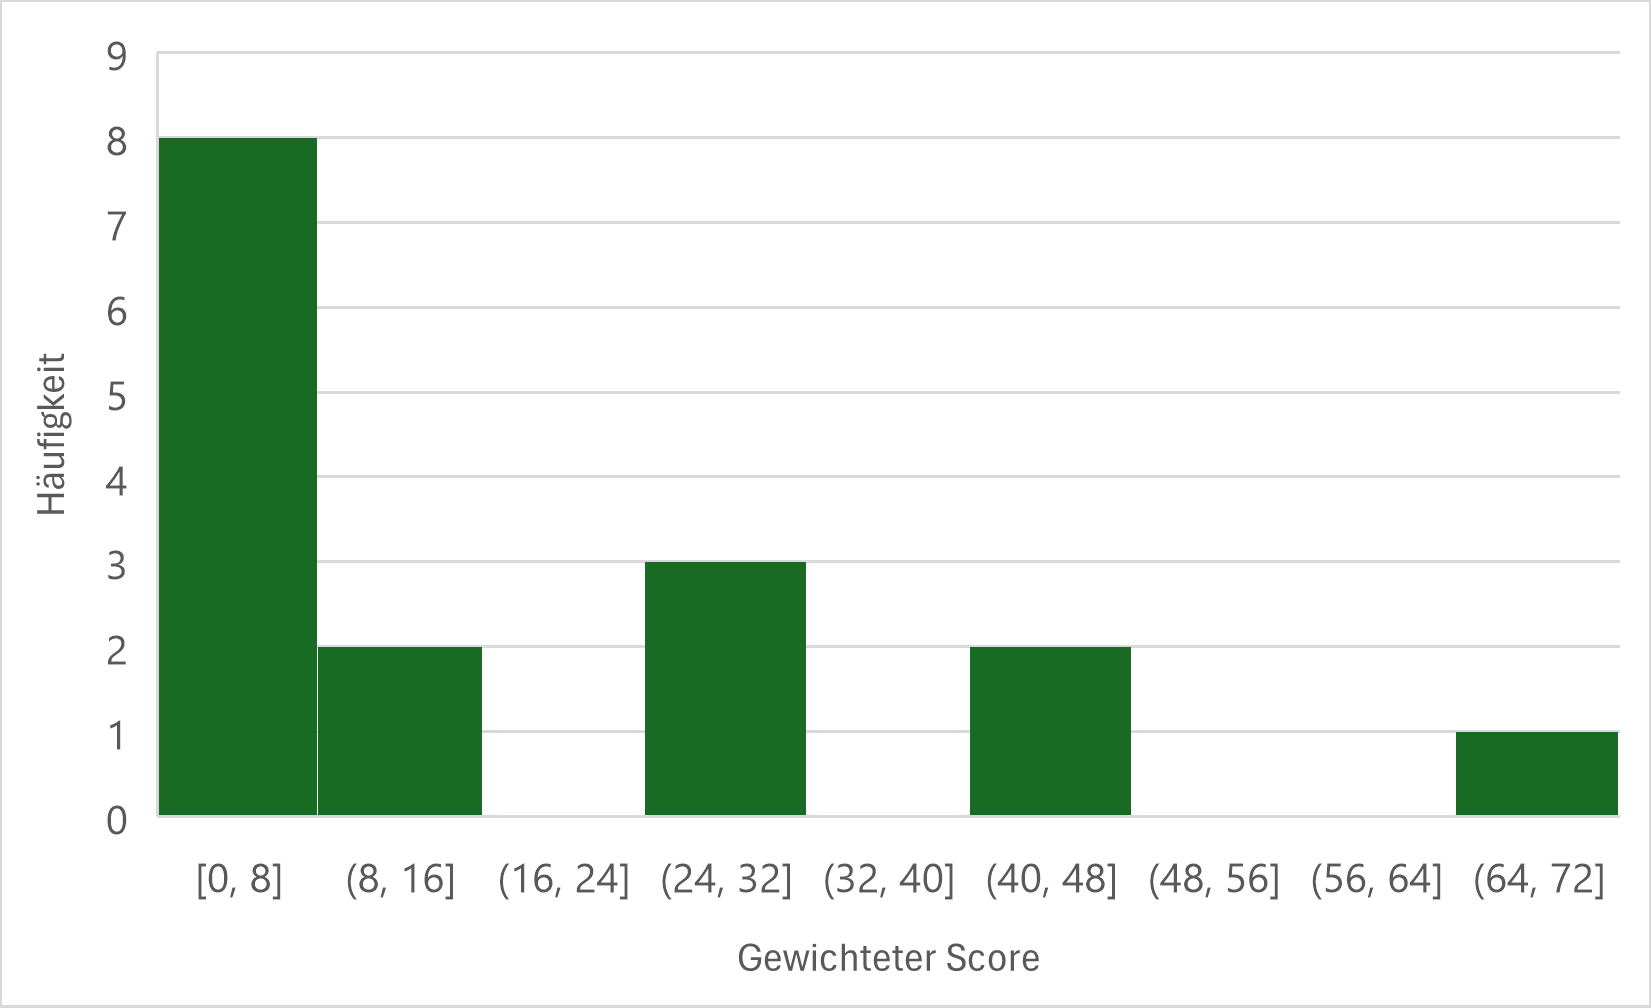
\includegraphics[width=0.99\textwidth]{images/Results/Histogramm-Disorientation-Scale-Item.png}
        \caption{Item Scanning}
        \label{fig:histoDisorientationItem}   
    \end{subfigure}%
    \begin{subfigure}{.5\textwidth}
        \centering
        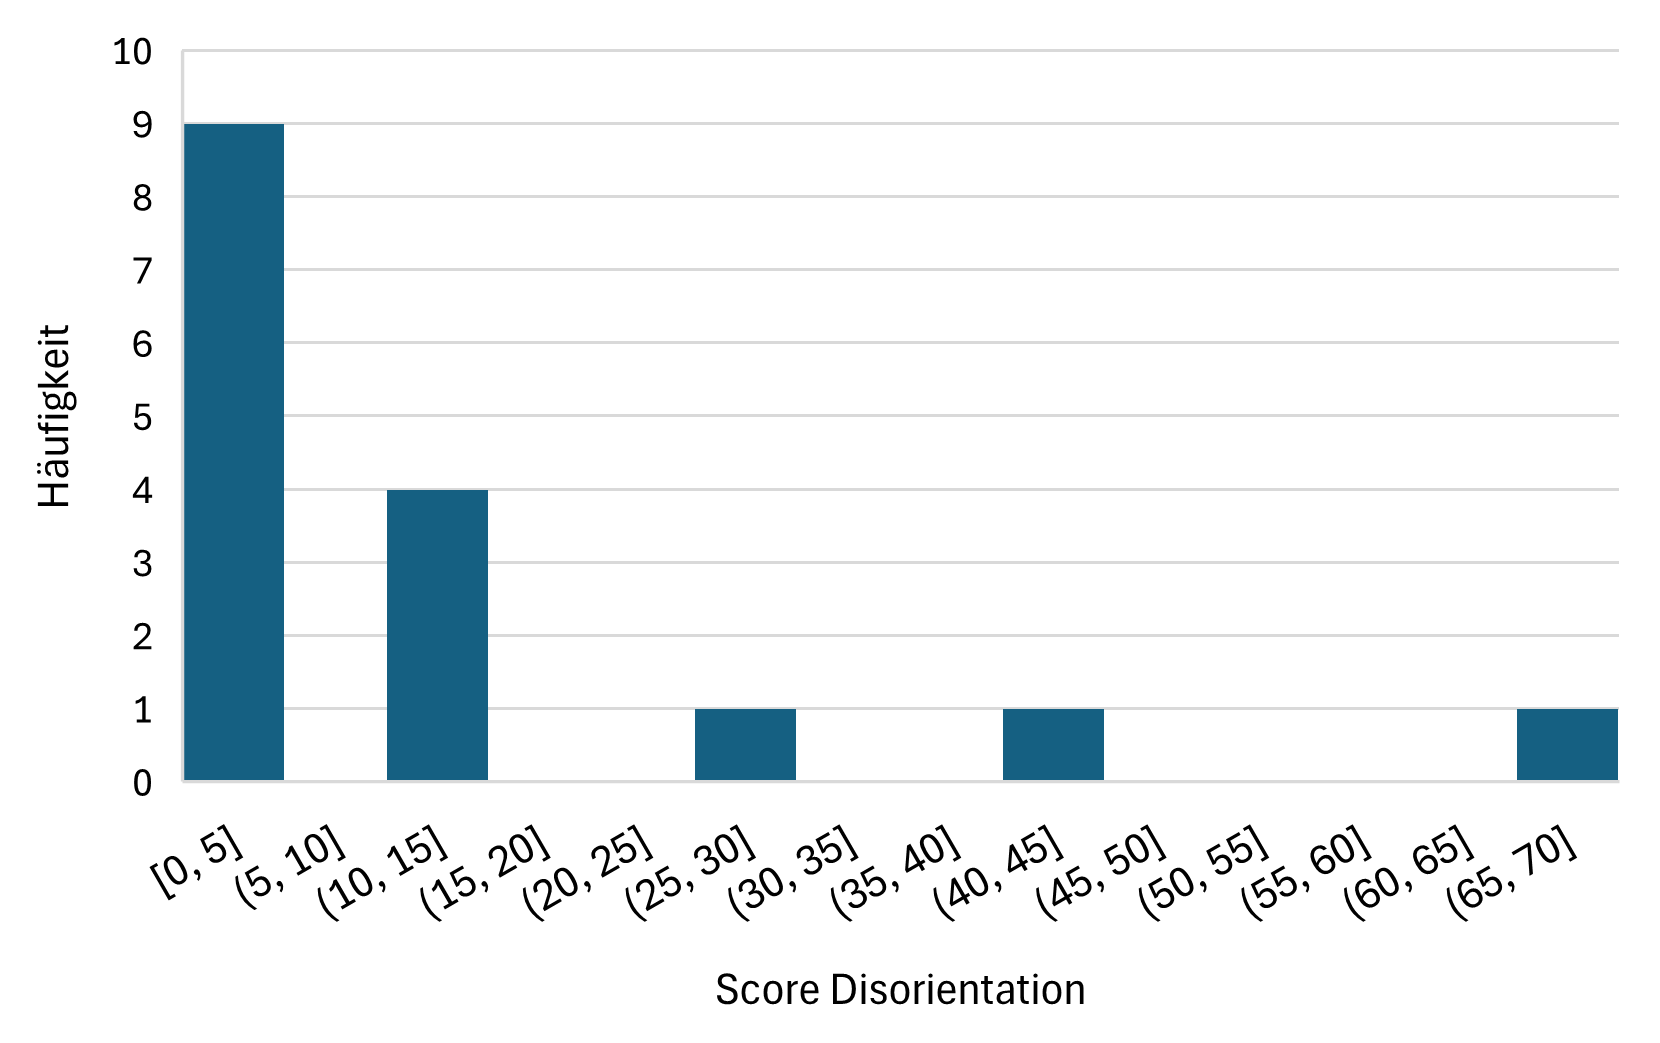
\includegraphics[width=0.99\textwidth]{images/Results/Histogramm-Disorientation-Scale-Cartesian.png}
         \caption{Cartesian Scanning}
         \label{fig:histoDisorientationCartesian}
    \end{subfigure}
    \caption{Verteilung der Scores der SSQ Disorientation Scale beider Verfahren}
    \label{fig:histoDisorientation}
\end{figure}

In der Kategorie Desorientierung (vgl. \autoref{fig:histoDisorientation}) zeigten beim Item Scanning acht Personen keine Symptome. Zwei Teilnehmende erreichten einen Score zwischen 10 und 15. Sechs Personen erreichten einen Score über 25, wobei eine Person sogar einen Score größer 60 erreichte. Der Mittelwert der Scores dieser Kategorie für das Item Scnning liegt bei 16,530 (Standardabweichung: 21,092) (vgl. \autoref{fig:tableErgebnisseSSQ}). Beim Cartesian Scanning blieben neun Personen symptomfrei, während vier Personen einen Score zwischen 10 und 15 erreichten. Nur drei Personen erreichten einen Score über 25, wobei eine Person soagr einen Score von 65 überschritt. Der Mittelwert der Scores dieser Kategorie liegt bei 12,180 (Standardabweichung: 19,604) (vgl. \autoref{fig:tableErgebnisseSSQ}).

\subsection{Ablenkung durch die Verfahren}

Die Ergebnisse zur Ablenkung bzw. Presence wurden anhand von drei Fragen erhoben, deren Mittelwerte für beide Verfahren in der \autoref{fig:presence} dargestellt sind.

\begin{figure}[tbh]
    \centering
    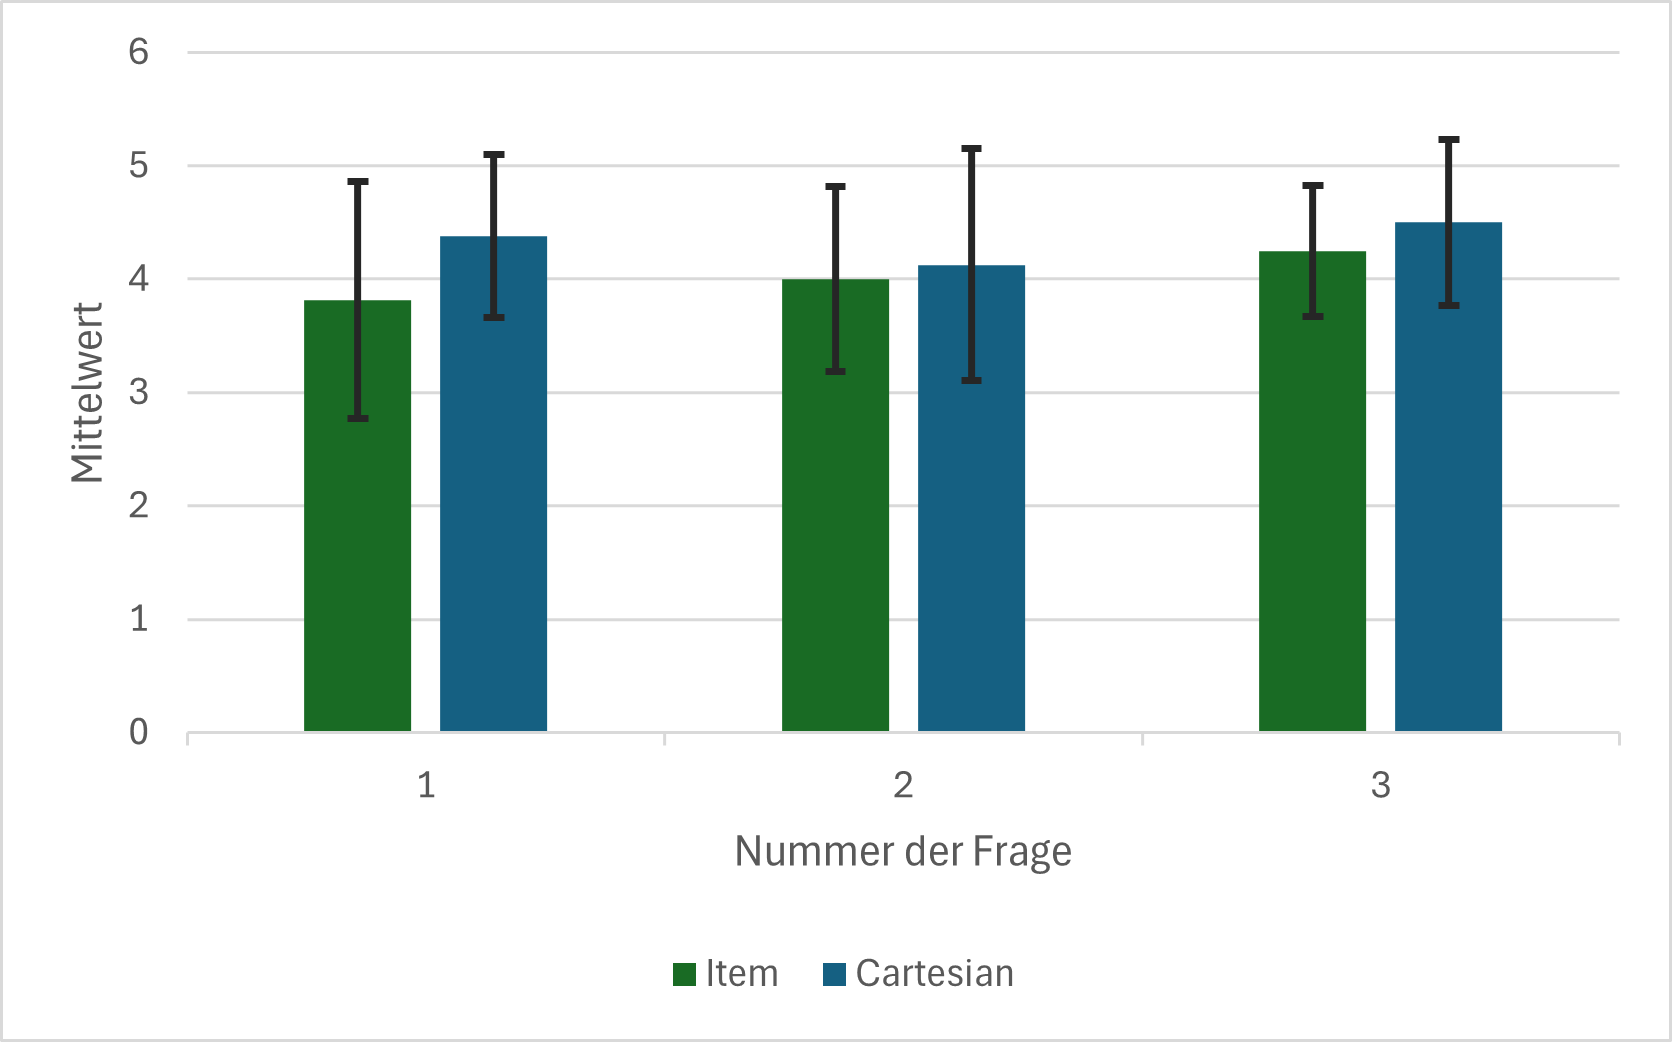
\includegraphics{images/Results/Fragen-zur-Presence-Ablenkung.png}
    \caption{Fragen zur Presence/Ablenkung}
    \label{fig:presence}
\end{figure}

\textit{Frage 1:} Wie sehr warst Du in die Erfahrung der virtuellen Umgebung involviert?
Die Bewertungen für das Item Scanning zeigen einen Mittelwert von 3,813 (Standardabweichung: 1,047). Für das Cartesian Scanning liegt der Mittelwert bei 4,375 (Standardabweichung: 0,719).

\textit{Frage 2:} Wie gut konntest Du Dich auf die zugewiesenen Aufgaben oder erforderlichen Tätigkeiten konzentrieren und nicht auf die Mechanismen, die zur Ausführung dieser Aufgaben oder Tätigkeiten genutzt werden?
Bei dieser Frage erreicht das Item Scanning einen Mittelwert von 4,000 (Standardabweichung: 0,817), während das Cartesian Scanning einen Mittelwert von 4,125 (Standardabweichung: 1,025) aufweist.

\textit{Frage 3:} Wie gut konntest Du Dich auf den Inhalt und die visuellen Darstellungen in der Szene konzentrieren?
Die Ergebnisse für das Item Scanning zeigen einen Mittelwert von 4,250 (Standardabweichung: 0,577). Beim Cartesian Scanning wird ein Mittelwert von 4,500 (Standardabweichung: 0,730) erzielt.

\subsection{Geschwindigkeit und Effizienz}

Die durchschnittlichen Zeiten für die Durchführung der Evaluationsabschnitte zeigen Unterschiede zwischen den beiden Verfahren, dargestellt in \autoref{fig:zeit} Beim Item Scanning benötigten die Teilnehmenden im technischen Abschnitt durchschnittlich 6 Minuten und 42 Sekunden (Standardabweichung = 1 Minute und 26 Sekunden). Im inhaltsbasierten Abschnitt betrug die benötigte Zeit durchschnittlich 5 Minuten und 35 Sekunden (Standardabweichung = 1 Minute und 43 Sekunden).
Beim Cartesian Scanning hingegen betrug die für den technischen Abschnitt benötigte Zeit durchschnittlich 8 Minuten und 5 Sekunden (Standardabweichung = 1 Minute und 41 Sekunden). Für den inhaltsbasierten Abschnitt wurden durchschnittlich 8 Minuten 50 Sekunden benötigt (Standardabweichung = 2 Minuten 52 Sekunden).

\begin{figure}[tbh]
    \centering
    \includegraphics{images/Results/Benötigte-Zeit-Evaluationsabschnitte.png}
    \caption{Benötigte Zeit zum Durchlaufen der Evaluationsabschnitte}
    \label{fig:zeit}
\end{figure}

Für die Auswertung der Geschwindigkeiten wurden die Interaktionsgeschwindigkeiten aus den Log-Files pro Person zusammengefasst. Daraus wurden Mittelwerte, Varianzen und Spannweiten berechnet, sowohl getrennt für jeden Evaluationsabschnitt als auch zusammengefasst für beide Abschnitte. Die Ergebnisse sind in der \autoref{fig:InteraktionsgeschwindigkeitenTable} aufgezigt sowie in der \autoref{fig:Interaktionsgeschwindigkeiten} visualisiert. 

Beim Item Scanning beträgt die durchschnittliche Interaktionsgeschwindigkeit im technischen Abschnitt 4.617 Sekunden (Varianz = 0.381; Spannweite = 2.064). Dagegen ist die Interaktionsgeschwindigkeit im inhaltsbasierten Abschnitt mit 2,927 Sekunden kürzer (Varianz = 0,522; Spannweite = 2,274). Über beide Abschnitte hinweg ergibt sich eine durchschnittliche Interaktionsgeschwindigkeit von 3,862 Sekunden (Varianz = 0,293; Spannweite = 1,917).
Beim Cartesian Scanning werden im technischen Abschnitt durchschnittlich 8,733 Sekunden (Varianz = 1,733; Spannweite = 4,840) zur Interaktion benötigt. Im inhaltsbasierten Abschnitt beträgt die mittlere Interaktionsgeschwindigkeit 7,404 Sekunden (Varianz = 5,616; Spannweite = 7,340). Über beide Abschnitte hinweg ergibt sich eine Interaktionsgeschwindigkeit von 8,004 Sekunden (Varianz = 3,383; Spannweite = 5,603).

\begin{figure}[tbh]
    \centering
    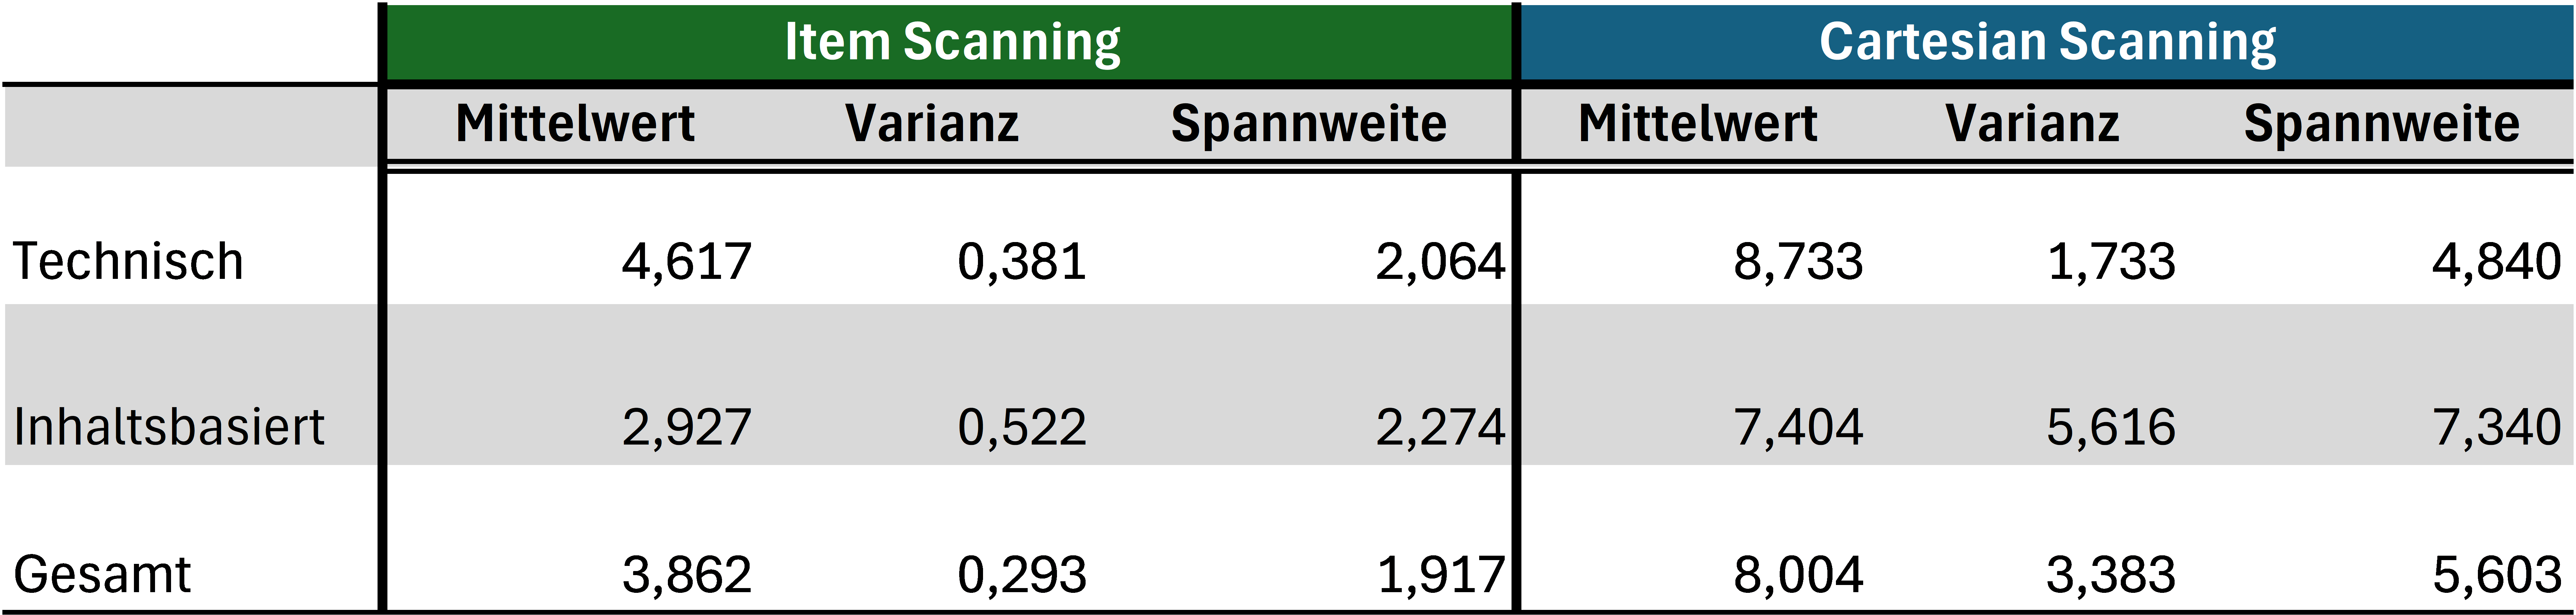
\includegraphics[width=0.95\textwidth]{images/Results/Interaktionsgeschwindigkeiten-Table.png}
    \caption{Tabelle der Interaktionsgeschwindigkeiten beider Verfahren nach Evalauationsabschnitt}
    \label{fig:InteraktionsgeschwindigkeitenTable}
\end{figure}

\begin{figure}[tbh]
    \centering
    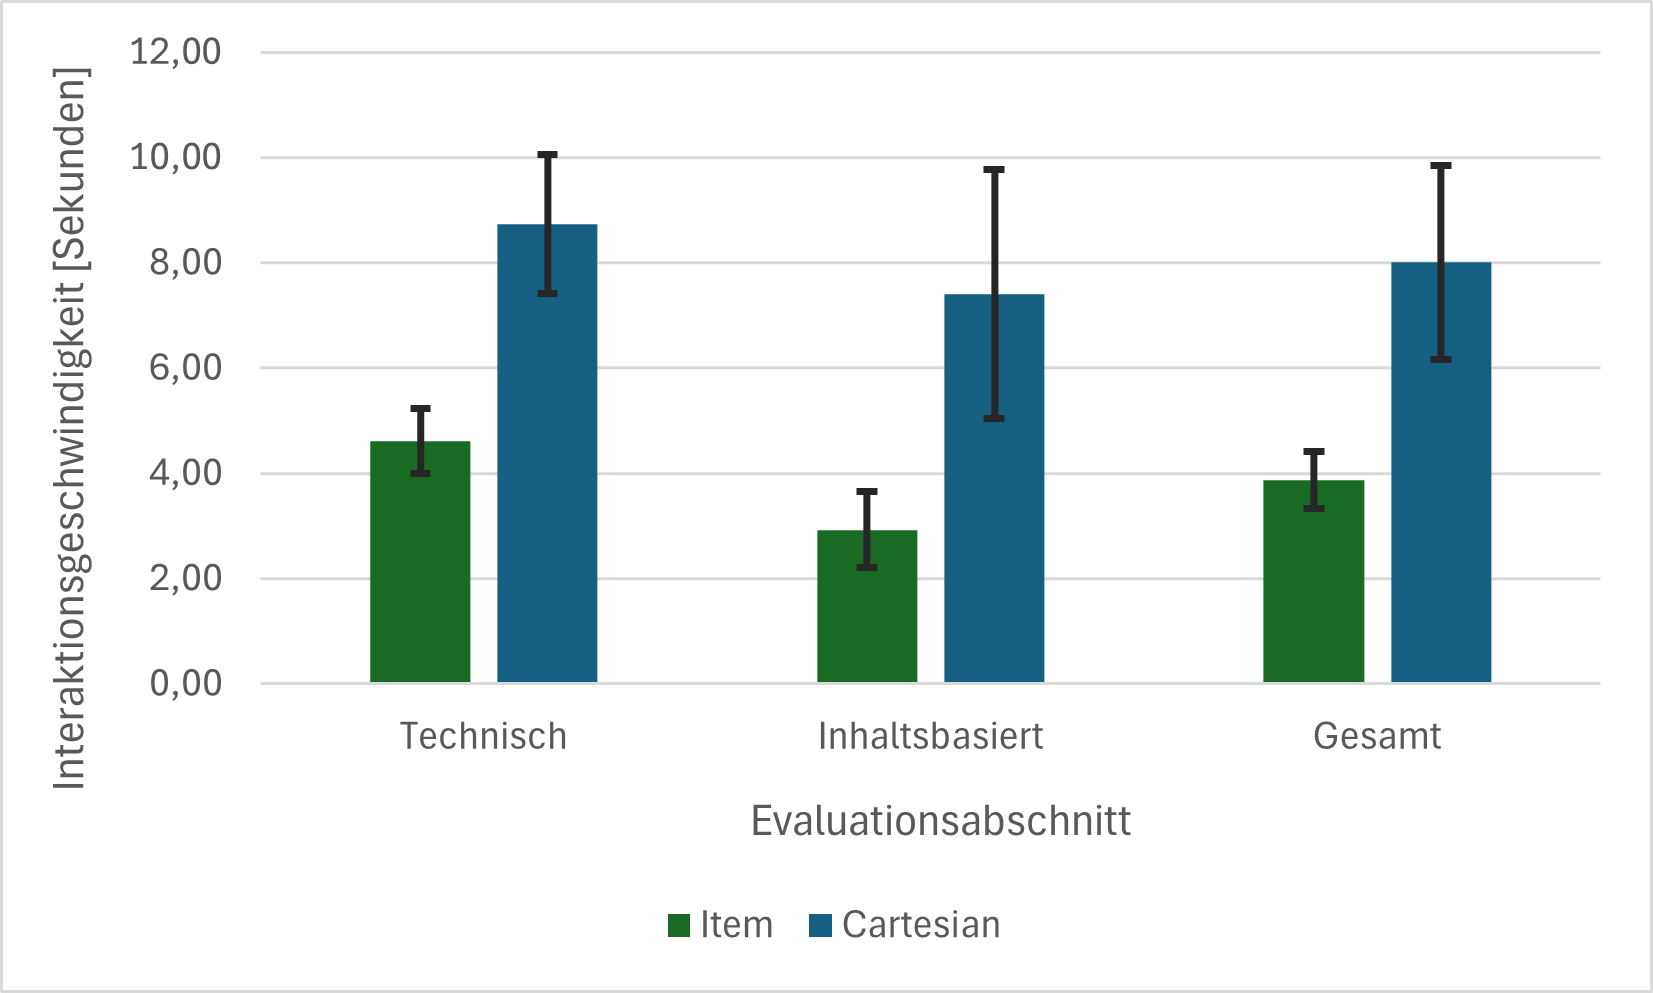
\includegraphics[width=0.75\textwidth]{images/Results/Interaktionsgeschwindigkeiten.png}
    \caption{Darstellung der mittleren Interaktionsgeschwindigkeiten beider Verfahren nach Evalauationsabschnitt}
    \label{fig:Interaktionsgeschwindigkeiten}
\end{figure}

Um die Veränderung der Interaktionsgeschwindigkeit über die Zeit bzw. über die Anzahl der durchgeführten Interaktionen zu untersuchen, wurde eine lineare Regressionsanalyse durchgeführt. Regressionsanalyse durchgeführt und anschließend die Korrelation zwischen den beiden Variablen berechnet. Die Ergebnisse werden in \autoref{fig:RegressionskoeffizientenTable} aufgezeigt. Der Regressionskoeffizient beschreibt die durchschnittliche Veränderung der Interaktionszeit in Abhängigkeit von der Anzahl der bereits durchgeführten Interaktionen. Der Korrelationskoeffizient gibt an, wie eng der Zusammenhang zwischen den Variablen ist. 
Beim Item Scanning ergibt sich für den technischen Abschnitt ein mittlerer Regressionskoeffizient von -0,839 (Varianz = 0,503) bei einem Korrelationskoeffizienten von -0,219. Im inhaltsbasierten Abschnitt beträgt der mittlere Regressionskoeffizient -0,391 (Varianz = 0,754) bei einem Korrelationskoeffizienten von -0,066. Über beide Abschnitte hinweg ergibt sich ein mittlerer Regressionskoeffizient von -2,539 (Varianz = 1,105) und ein Korrelationskoeffizient von -0,263.
Beim Cartesian Scanning ergibt sich für den technischen Abschnitt ein durchschnittlicher Regressionskoeffizient von 0,180 (Varianz = 0,326) mit einem Korrelationskoeffizienten von 0,038. Im inhaltsbasierten Abschnitt beträgt der Regressionskoeffizient 0,241 (Varianz = 1,177) und der Korrelationskoeffizient -0,019. Über beide Abschnitte hinweg beträgt der Regressionskoeffizient -0,492 (Varianz = 1,461) und der Korrelationskoeffizient -0,085.


\begin{figure}[tbh]
    \centering
    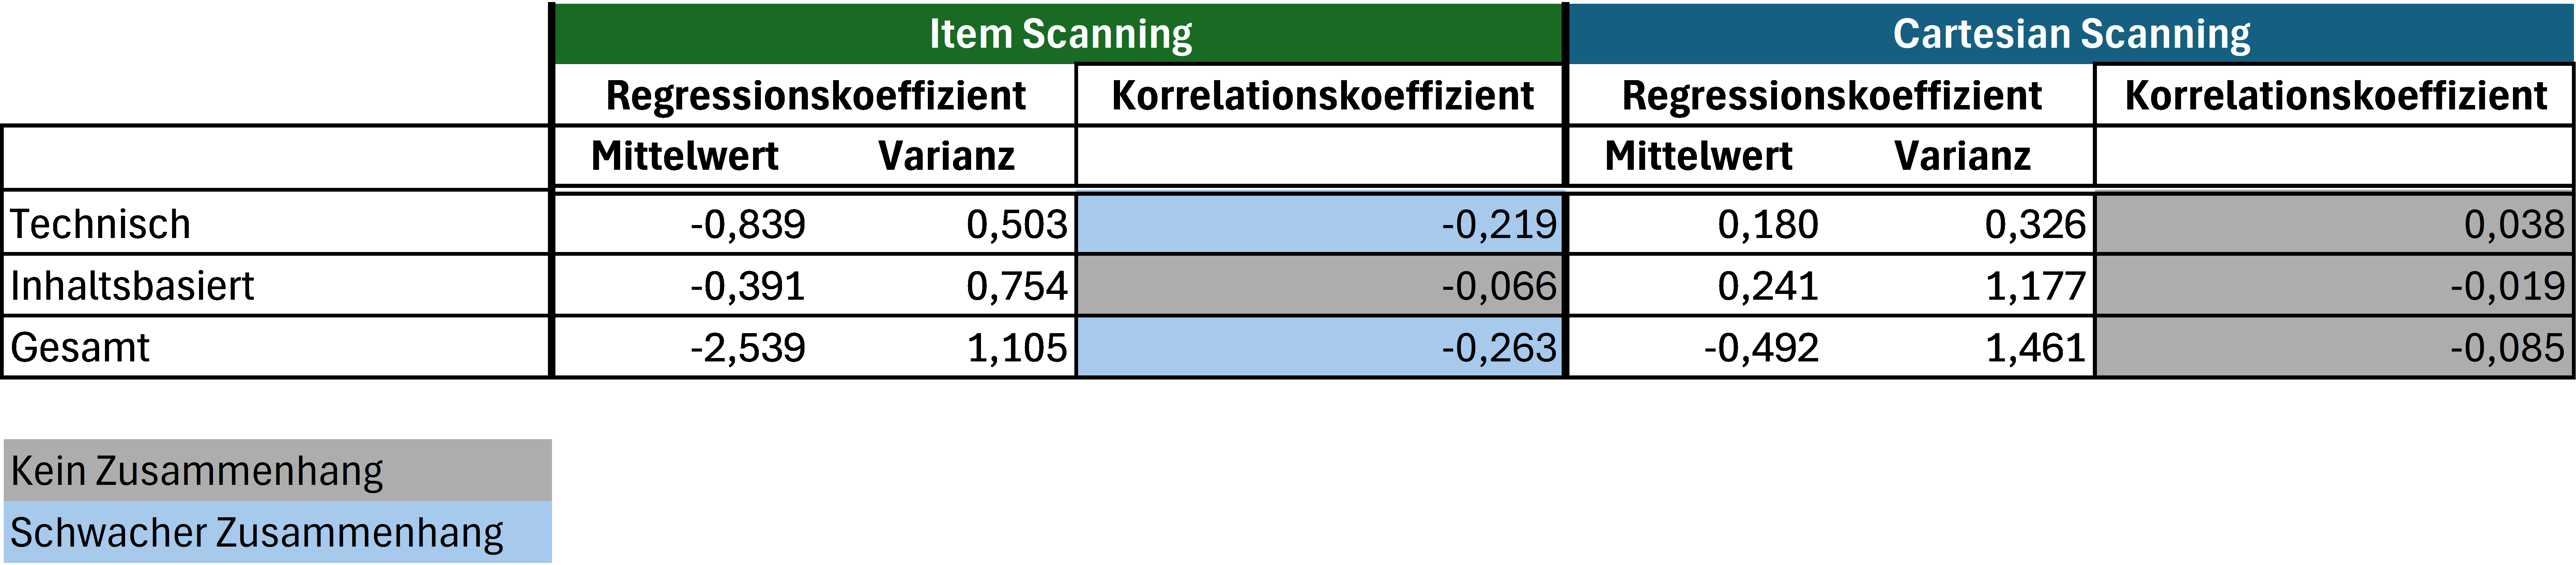
\includegraphics[width=0.95\textwidth]{images/Results/Regressionskoeffizienten-Korrelation-Table-Lernkurve-Geschwindigkeit.png}
    \caption{Regressionskoeffizienten Lernkurve}
    \label{fig:RegressionskoeffizientenTable}
\end{figure}

Neben der Interaktionsgeschwindigkeit wurde auch die Anzahl der benötigten Scanning Zyklen pro Interaktion im Log-File erfasst. Die \autoref{fig:zyklen} zeigt die Ergebnisse bezüglich der Zyklen für das Item Scanning. Im technischen Abschnitt wurden durchschnittlich 1,542 Zyklen pro Eingabe benötigt (Varianz = 0,007; Spannweite = 0,332). Im inhaltsbasierten Abschnitt hingegen lag der Mittelwert bei 1,423 (Varianz = 0,021; Spannweite = 0,481).

Auch für das Cartesian Scanning wurde die Anzahl der benötigten Durchläufe der Scaninng-Linien ausgegeben. %hier noch die Erklärung ergänzen! 

\begin{figure}[tbh]
    \centering
    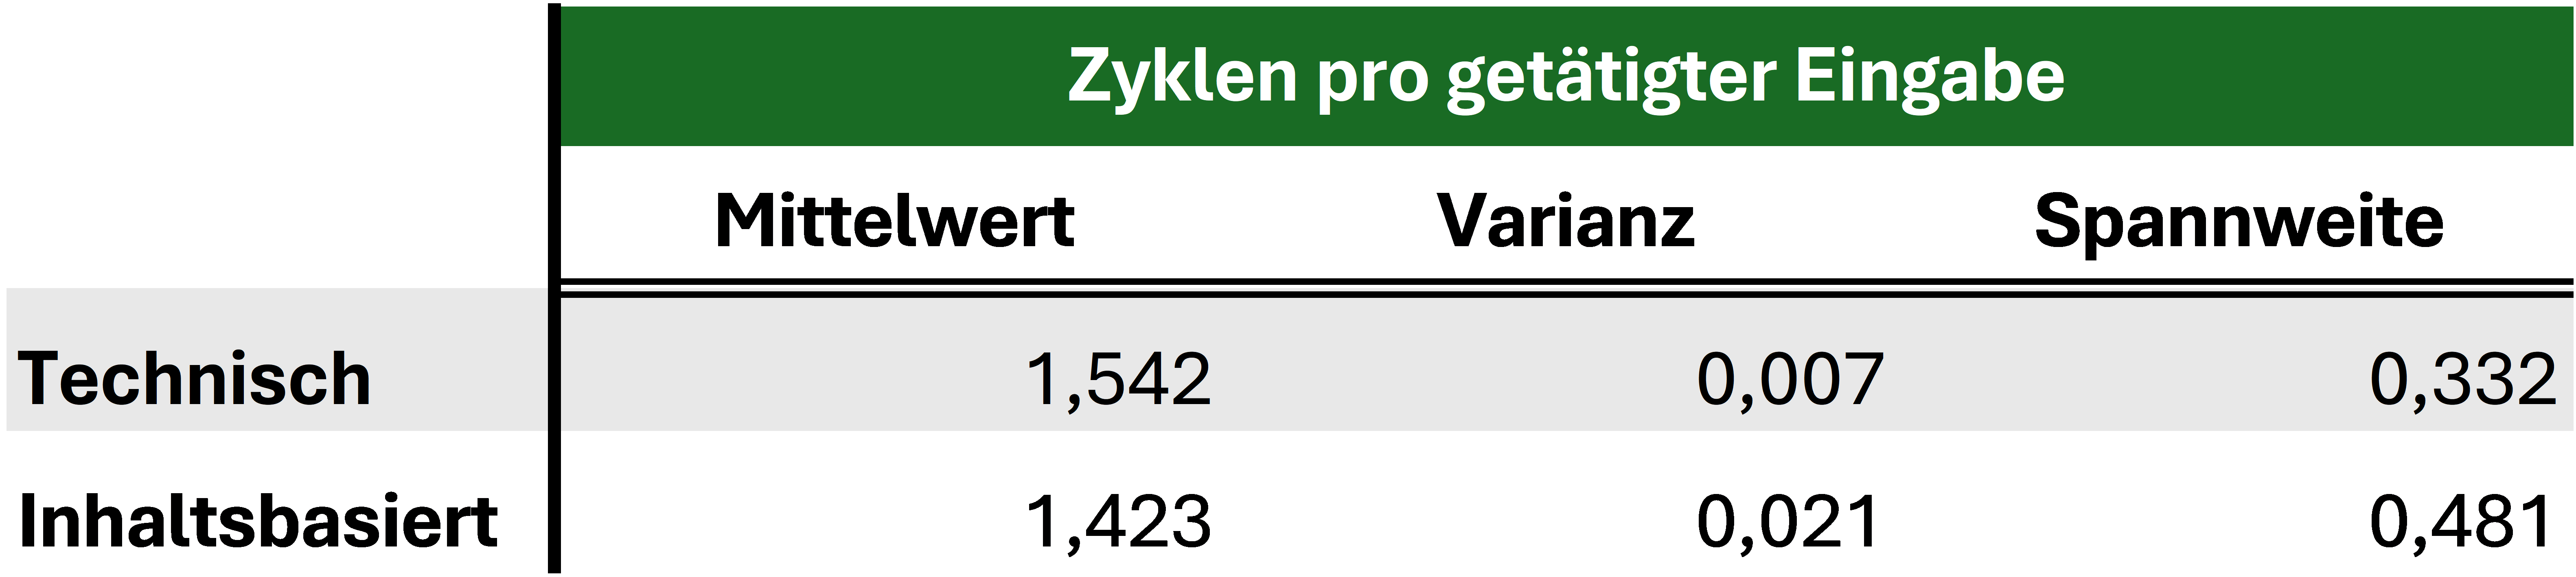
\includegraphics{images/Results/Zyklen-Item.png}
    \caption{Benötigte Scanning-Zyklen pro Interaktion beim Item Scanning}
    \label{fig:zyklen}
\end{figure}

\subsection{Robustheit}

In beiden Evalauationsabschnitten wurden die aufgetretenen Fehler im Evaluationsprotokoll erfasst. Als Fehler werden in diesem Zusammenhang Eingaben verstanden, die nicht zum gewünschten Ergebnis geführt haben. 

Die Ergebnisse des Item Scannings sind in \autoref{fig:anzahlFehlerItem} dargestellt. Im technischen Abschnitt (vgl. \autoref{fig:anzahlFehlerItemTechnisch}) traten bei der Mehrheit der Teilnehmenden Fehler auf. Nur drei Personen konnten den Abschnitt ohne Fehler abschließen. Sieben Personen machten einen Fehler, zwei Personen machten jeweils drei Fehler. Eine Person hat fünf Fehler gemacht. Somit wurden in diesem Abschnitt über alle Testpersonen hinweg insgesamt 18 Fehler erfasst.
Im inhaltsbasierten Abschnitt (vgl. \autoref{fig:anzahlFehlerItemInhalt}) haben sechs Personen keinen Fehler gemacht, während weitere sechs Personen jeweils einen Fehler machten. Vier Personen machten zwei Fehler. Keine Testperson hat in diesem Abschnitt mehr als zwei Fehler gemacht. Insgesamt wurden in diesem Abschnitt 14 Fehler verzeichnet.

\begin{figure}[tbh]
    \centering
    \begin{subfigure}{.5\textwidth}
        \centering
        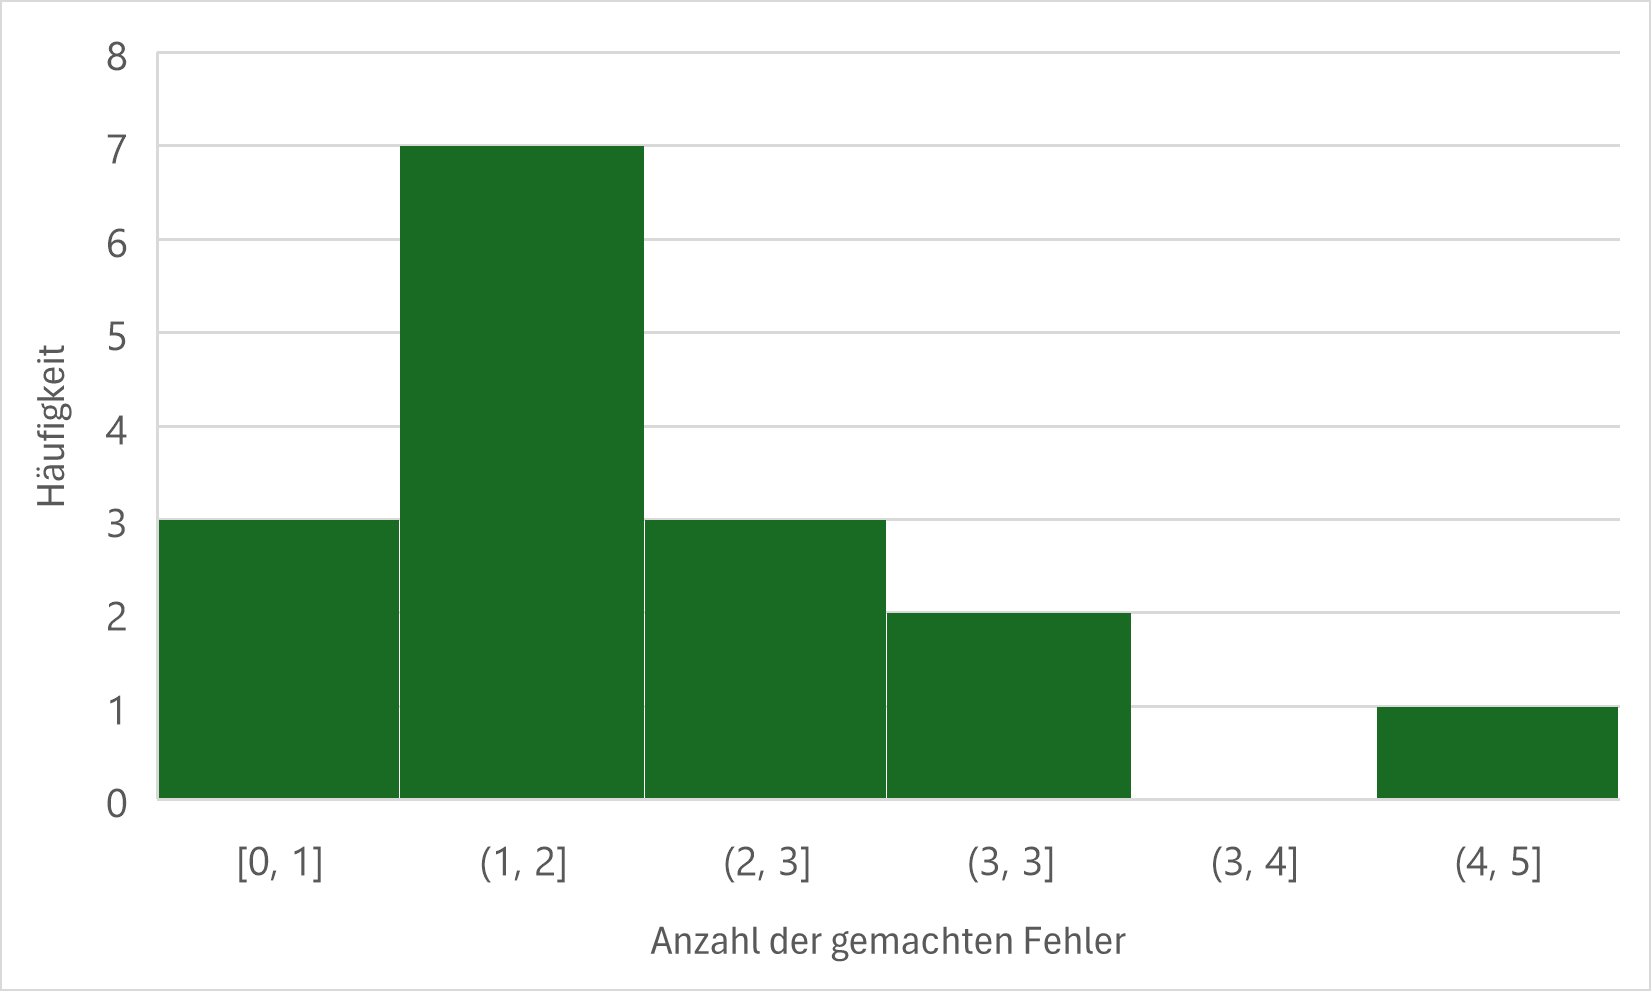
\includegraphics[width=0.95\textwidth]{images/Results/Histogramm-Anzahl-Fehler-technisch-item.png}
        \caption{Technischer Abschnitt}
        \label{fig:anzahlFehlerItemTechnisch}
    \end{subfigure}%
    \begin{subfigure}{.5\textwidth}
        \centering
        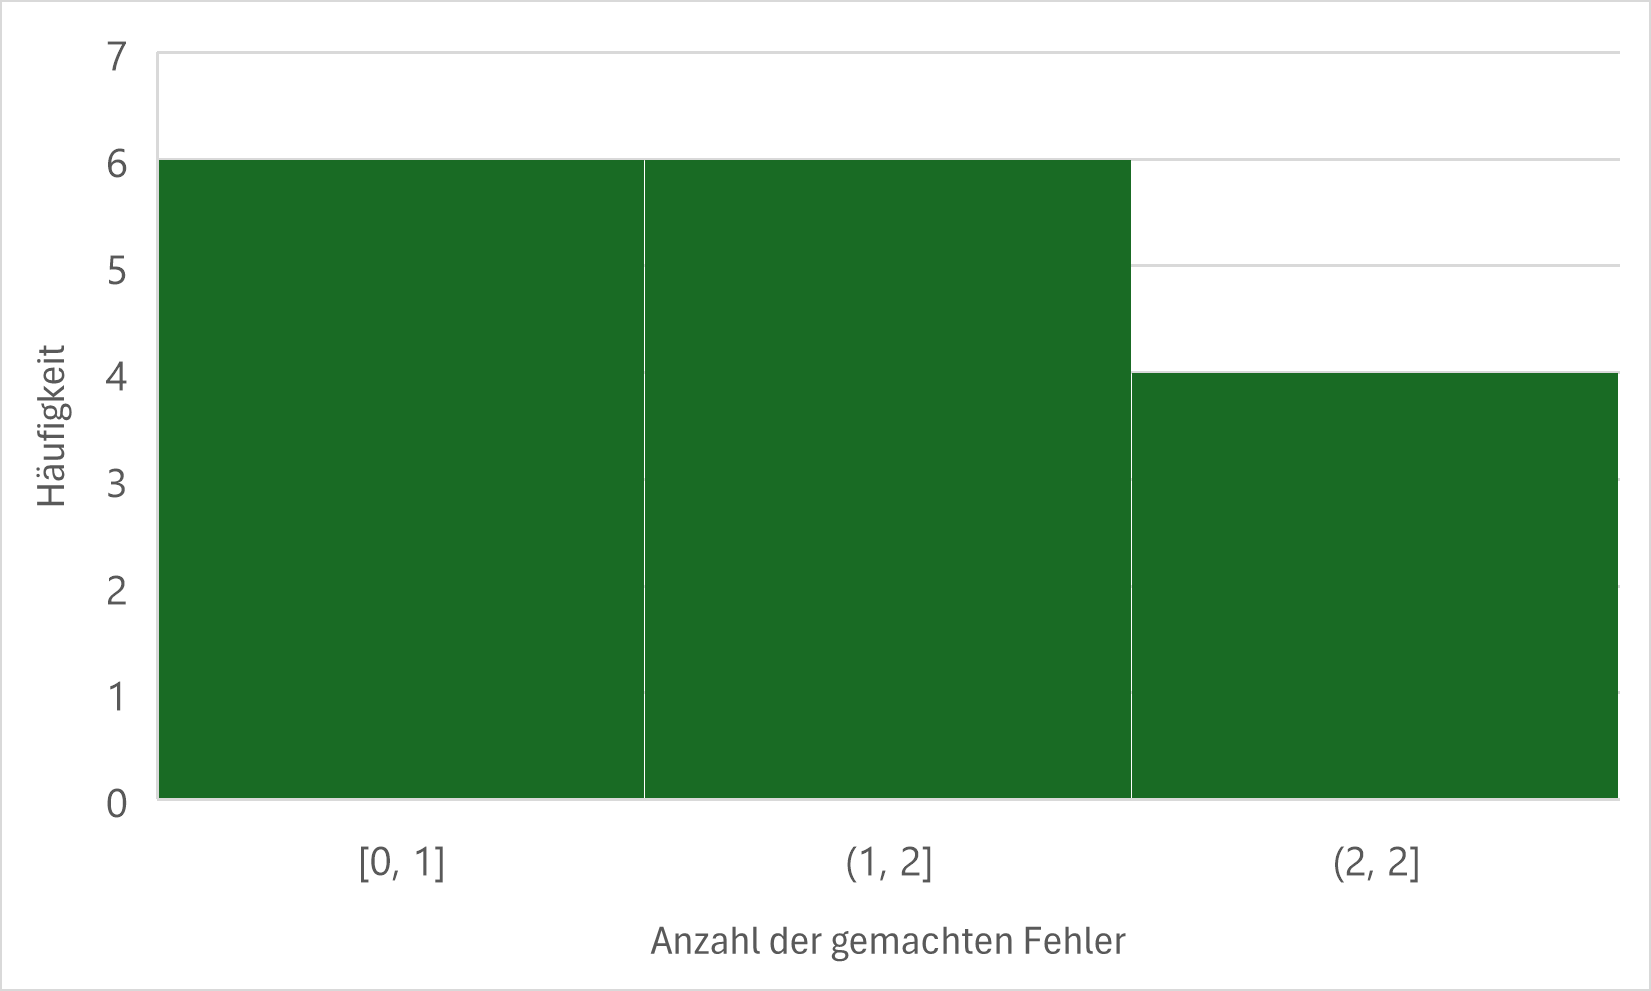
\includegraphics[width=0.95\textwidth]{images/Results/Histogramm-Anzahl-Fehler-inhalt-item.png}
        \caption{Inhaltsbasierter Abschnitt}
        \label{fig:anzahlFehlerItemInhalt}
   \end{subfigure}
   \caption{Häufigkeiten der Anzahl gemachter Fehler im Item Scanning}
   \label{fig:anzahlFehlerItem}
\end{figure}
\

Im Evaluationsprotokoll wurde für jeden aufgetretenen Fehler der jeweilige Grund vermerkt. Die beim Item Scanning aufgetretenen Gründe sind in \autoref{fig:gründeFehlerItem} aufgeführt. Es ist zu erkennen, dass die meisten Fehler auf Timing-Probleme zurückzuführen sind. Das bedeutet, dass Eingaben etwas zu früh oder etwas zu spät erfolgten und dadurch versehentlich das vorherige oder nachfolgende Item in der Scanning-Reihenfolge anstelle des Zielobjekts ausgewählt wurde. Zu späte Eingaben traten insbesondere bei der Navigation auf. Derartige Fehler traten bei 13 der 16 Testpersonen auf. Im technischen Abschnitt der Evaluation traten zudem Fehler auf, die auf Verständnisprobleme zurückzuführen sind. Vier Teilnehmenden war das Prinzip bzw. die Aufgabe zu Beginn nicht ganz klar, wodurch es zu fehlerhaften Eingaben kam. 

\begin{figure}[tbh]
    \centering
    \includegraphics{images/Results/Gründe-Fehler-Item.png}
    \caption{Gründe für Fehler beim Item Scanning}
    \label{fig:gründeFehlerItem}
\end{figure}

Die Ergebnisse des Cartesian Scanning sind in \autoref{fig:anzahlFehlerCartesian} dargestellt.
Den technischen Abschnitt (vgl. \autoref{fig:anzahlFehlerCartesianTechnisch}) konnten sieben Personen fehlerfrei abschließen. Drei Personen machten jeweils einen oder zwei Fehler, während jeweils eine Person drei, vier oder sechs Fehler machte. Insgesamt wurden in diesem Abschnitt über alle Testpersonen hinweg 22 Fehler erfasst. 
Im inhaltsbasierten Abschnitt (vgl. \autoref{fig:anzahlFehlerCartesianInhalt}) blieb die Hälfte der Testpersonen fehlerfrei. Fünf Personen machten jeweils einen Fehler, eine Person drei, eine Person vier und eine Person acht Fehler. Die Gesamtzahl der Fehler beträgt hier somit 20.

\begin{figure}
    \centering
    \begin{subfigure}{.5\textwidth}
        \centering
        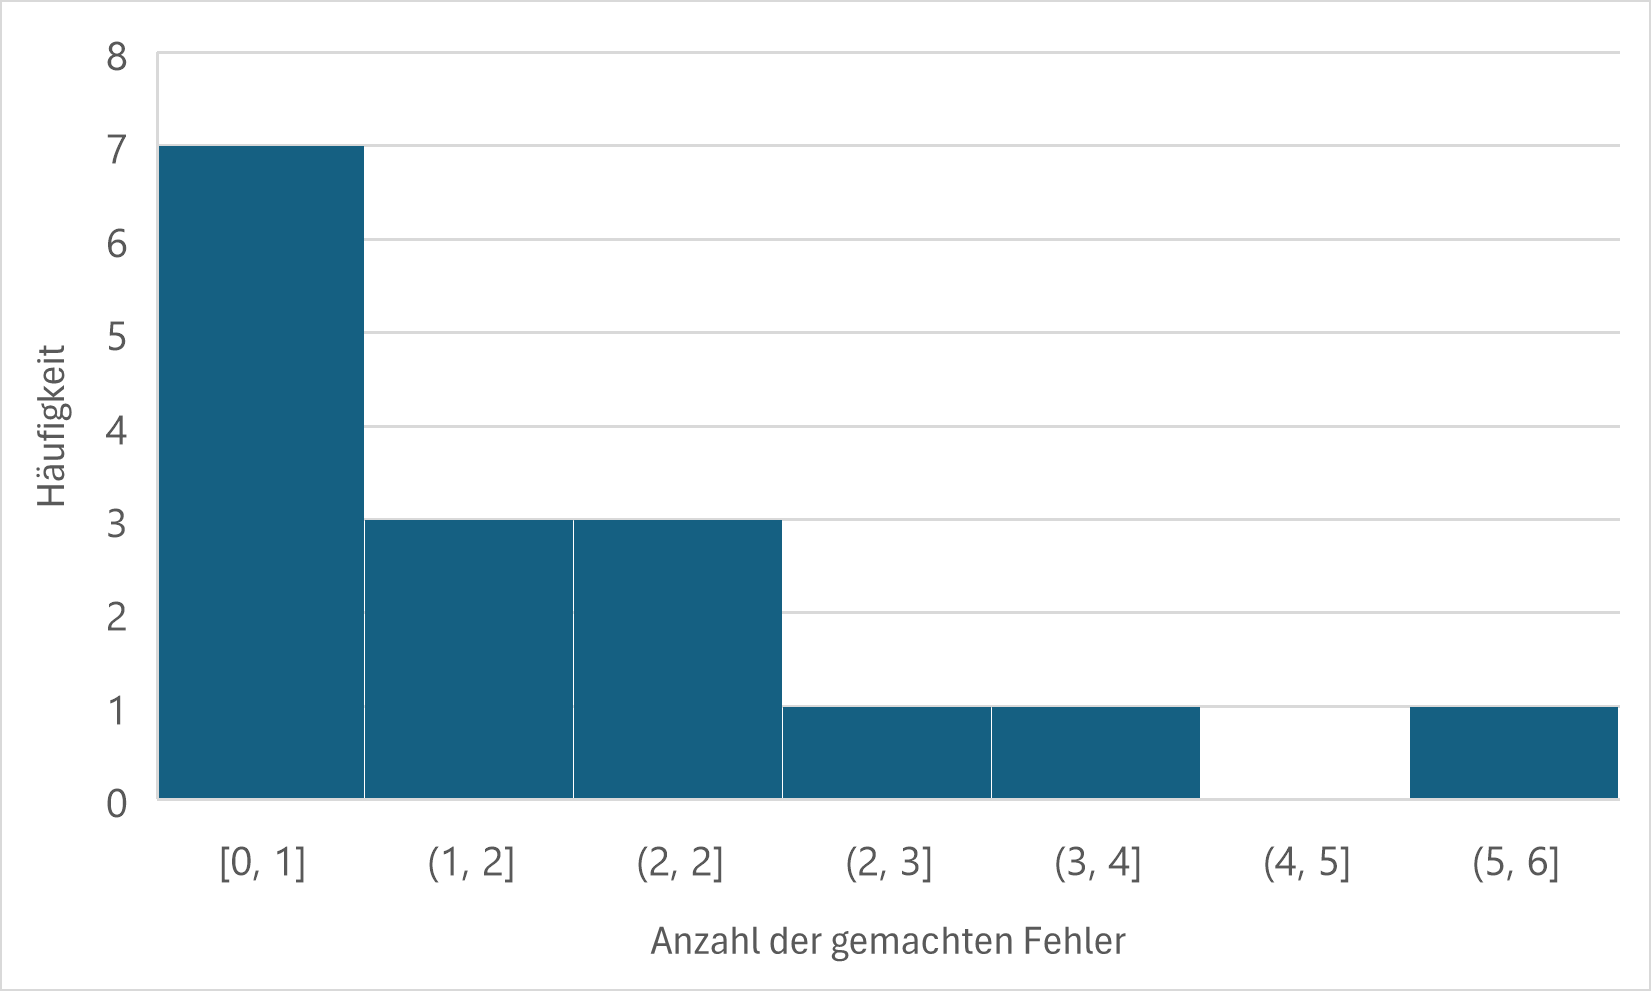
\includegraphics[width=0.95\textwidth]{images/Results/Histogramm-Anzahl-Fehler-technisch-cartesian.png}
        \caption{Technischer Abschnitt}
        \label{fig:anzahlFehlerCartesianTechnisch}
    \end{subfigure}%
    \begin{subfigure}{.5\textwidth}
        \centering
        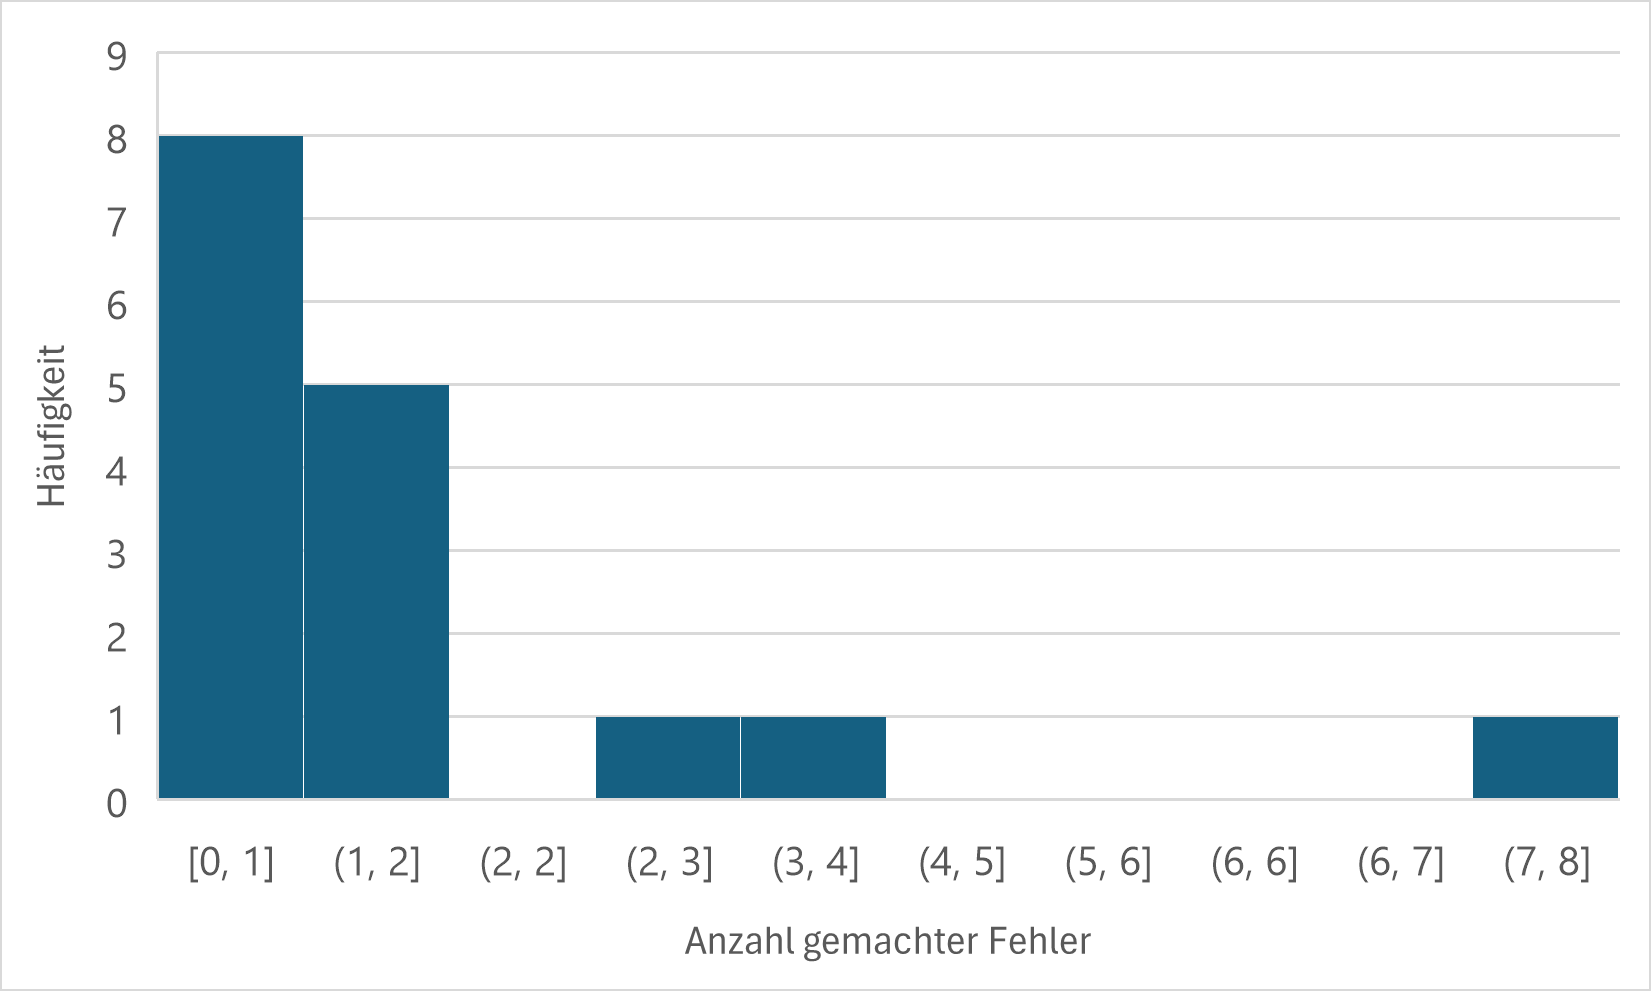
\includegraphics[width=0.95\textwidth]{images/Results/Histogramm-Anzahl-Fehler-inhalt-cartesian.png}
        \caption{Inhaltsbasierter Abschnitt}
        \label{fig:anzahlFehlerCartesianInhalt}
    \end{subfigure}
    \caption{Häufigkeiten der Anzahl gemachter Fehler beim Cartesian Scanning}
    \label{fig:anzahlFehlerCartesian}
\end{figure}

Die Gründe für Fehler beim Cartesian Scanning sind in \autoref{fig:gründeFehlerCartesian} dargestellt. Es ist zu erkennen, dass neun Personen versehentlich das HUD anstelle des beabsichtigten Objekts ausgewählt haben. Fünf Personen vergaßen den Moduswechsel, was dazu führte, dass statt einer Selektion weitere Navigationsschritte durchgeführt wurden. Drei Personen hatten Probleme beim Schließen von Bildern, da sie den Schließen-Button nicht wählen konnten. Eine Person hielt den Schalter für den Moduswechsel nicht lange genug gedrückt, sodass der Wechsel nicht ausgelöst wurde und weitere Navigationsschritte statt der gewünschten Selektion ausgeführt wurden. Eine Person selektierte versehentlich einen Wegpunkt, der hinter einem geöffneten Bild lag, obwohl eine leere Eingabe beabsichtigt war. 

\begin{figure}[tbh]
 \centering
\includegraphics[width=0.95\textwidth]{images/Results/Gründe-Fehler-Cartesian.png}
 \caption{Gründe für Fehler beim Cartesian Scanning}
 \label{fig:gründeFehlerCartesian}
\end{figure}

Beim Cartesian Scanning wurde zusätzlich die Häufigkeit von leeren Eingaben zur Korrektur von Fehlern, wie z.B. das Setzen der ersten Scanlinie an der falschen Position oder das Vergessen des Wechsels in den Navigationsmodus, erfasst. Die Ergebnisse sind in \autoref{fig:leereEingaben} dargestellt. 
Im technischen Abschnitt beträgt die durchschnittliche Anzahl leerer Eingaben 1.000 (Varianz = 2.933; Spannweite = 7.000). Im inhaltsbasierten Abschnitt liegt der Mittelwert mit 1.750 (Varianz = 6.200; Spannweite = 10.000) etwas höher.

\begin{figure}[tbh]
    \centering
    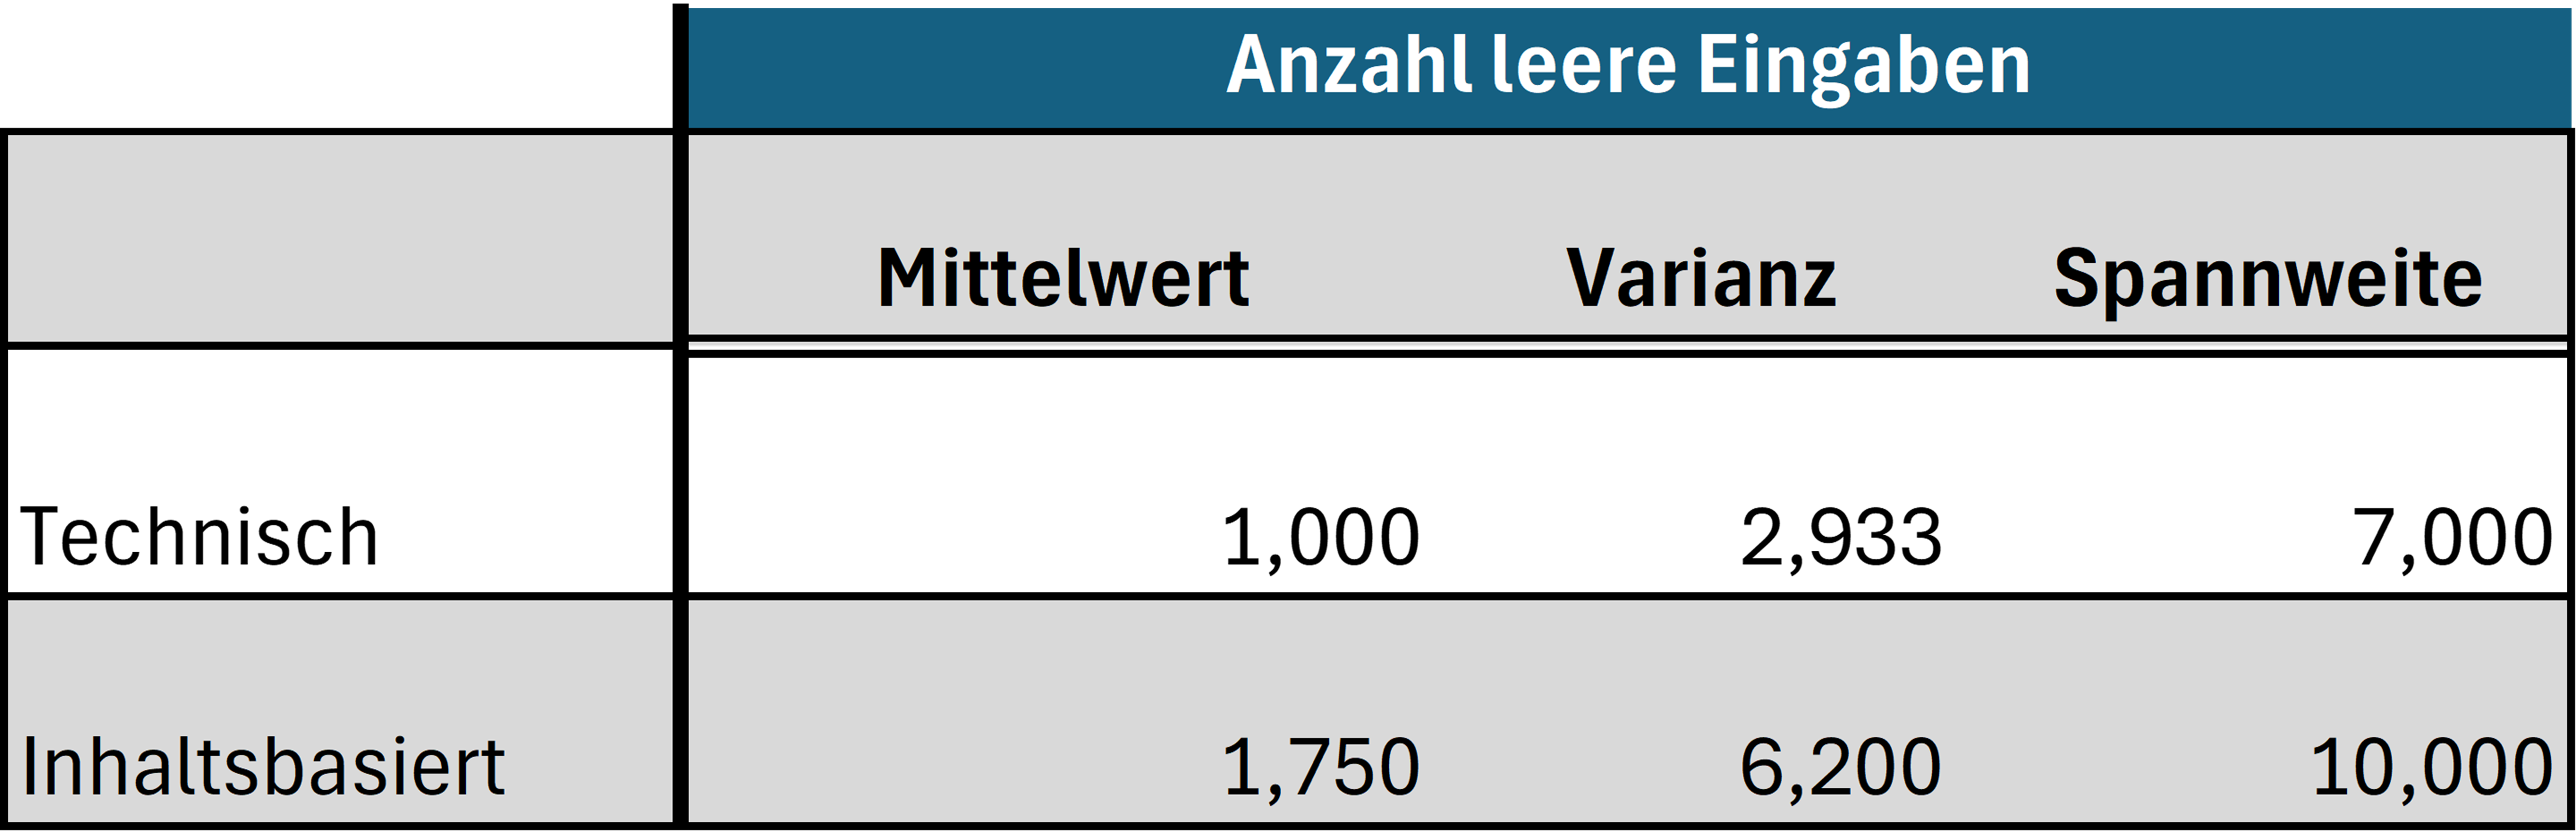
\includegraphics{images/Results/leereEingaben.png}
    \caption{Leere Eingaben beim Cartesian Scanning}
    \label{fig:leereEingaben}
\end{figure}

\subsection{Korrelationen und Zusammenhänge}

Neben der getrennten Auswertung der Ergebnisse der einzelnen Variablen und Faktoren wurden Korrelationsanalysen durchgeführt, um Zusammenhänge zwischen den Variablen zu untersuchen.

Zunächst wurde für das Cartesian Scanning untersucht, ob die Position der ausgewählten Objekte im Sichtfeld (x- und y-Koordinaten) einen signifikanten Einfluss auf die Interaktionsgeschwindigkeit hat. Die Ergebnisse sind in \autoref{fig:tableKorrPosGeschwindigkeit} zusammengefasst und in \autoref{fig:bubbleKorrPosGeschwindigkeit} visualisiert. 

\begin{figure}[tbh]
    \centering
    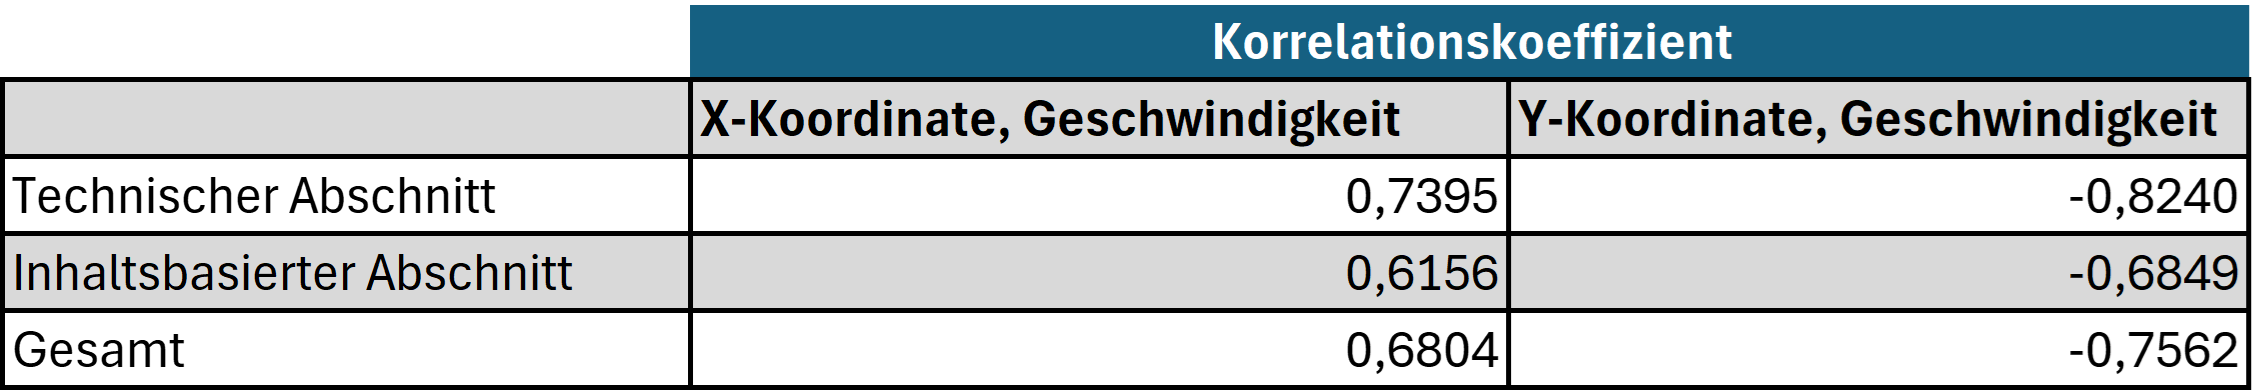
\includegraphics[width=0.95\textwidth]{images/Results/Korrelation-Position-Geschwindigkeit-Table.png}
    \caption{Zusammenhang Postion des Objekts im Sichtfeld und Selektionsgeschwindigkeit}
    \label{fig:tableKorrPosGeschwindigkeit}
\end{figure}

\begin{figure}
    \centering
    \begin{subfigure}{.5\textwidth}
        \centering
        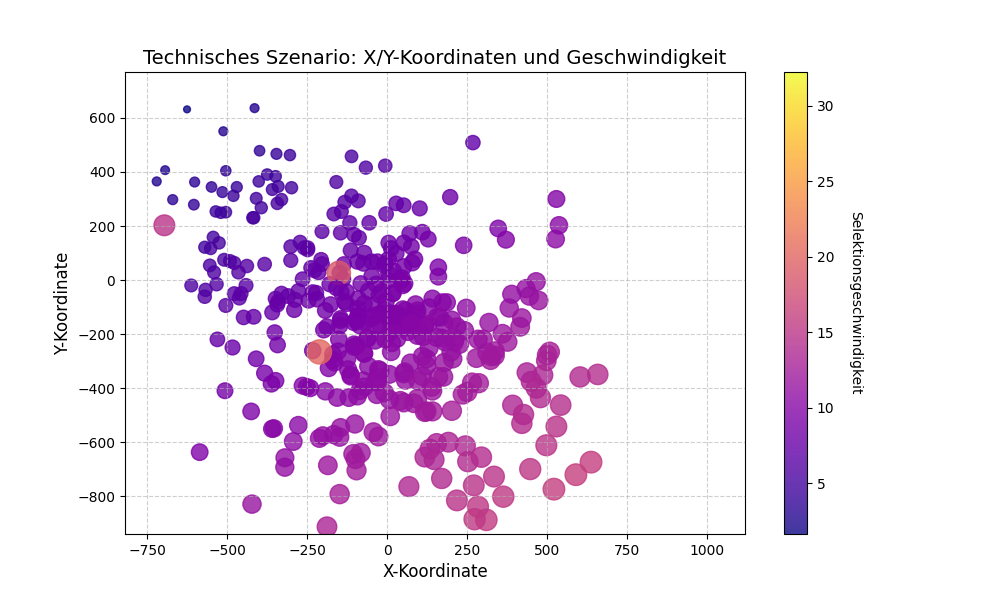
\includegraphics[width=0.95\textwidth]{images/Results/bubbleplot-technisch.png}
        \caption{Technischer Abschnitt}
        \label{fig:bubbleKorrPosGeschwindigkeitTechnisch}
    \end{subfigure}%
    \begin{subfigure}{.5\textwidth}
        \centering
        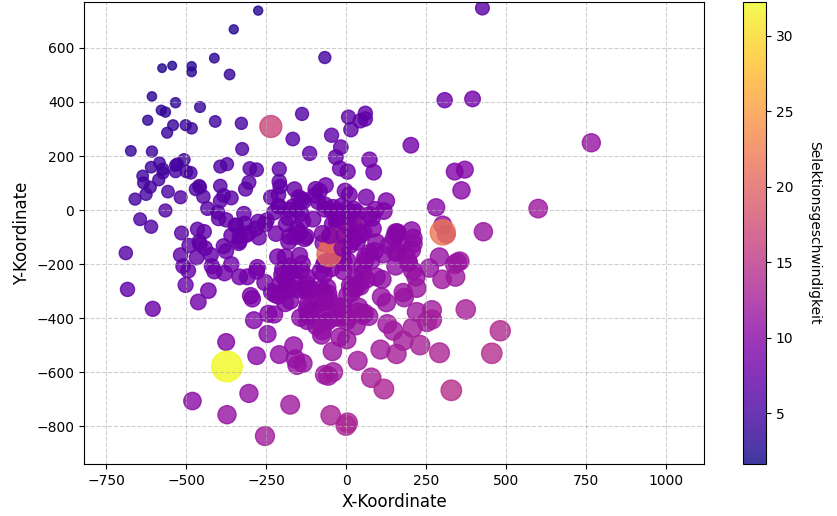
\includegraphics[width=0.95\textwidth]{images/Results/bubbleplot-inhalt.png}
        \caption{Inhaltsbasierter Abschnitt}
        \label{fig:bubbleKorrPosGeschwindigkeitInhalt}
    \end{subfigure}
    \caption{Zusammenhang zwischen der Position des Objektes im Sichtfeld und der Interaktionsgeschwindigkeit beim Cartesain Scanning}
    \label{fig:bubbleKorrPosGeschwindigkeit}
\end{figure}

Für den technischen Abschnitt zeigt sich eine positive Korrelation zwischen der horizontalen Position (x-Koordinate) und der Interaktionsgeschwindigkeit (Korrelationskoeffizient = 0,7395), während die vertikale Position (y-Koordinate) negativ mit der Geschwindigkeit korreliert (Korrelationskoeffizient = -0,8249). Ähnliche Tendenzen lassen sich im inhaltsbasierten Abschnitt beobachten, wo die Korrelationskoeffizienten für die x-Koordinate 0,6156 und für die y-Koordinate -0,6849 betragen. Werden beide Abschnitte zusammen betrachtet, ergeben sich Korrelationskoeffizienten von 0,6804 für die x-Koordinate und -0,7562 für die y-Koordinate. Alle Korrelationen zeigen dabei einen p-Wert <0,00. Die \autoref{fig:bubbleKorrPosGeschwindigkeit} veranschaulicht diese Zusammenhänge. Punkte, die eine schnelle Selektion repräsentieren, befinden sich oben links im Sichtfeld und sind klein und dunkelblau dargestellt. Mit zunehmender Entfernung nach rechts oder unten im Sichtfeld werden die Punkte größer und heller. Darüber hinaus ist in dieser Abbildung zu erkennen, dass die meisten Selektionen in der Mitte des Sichtfeldes durchgeführt wurden.

Anschließend wurde für beide Verfahren untersucht, ob es Korrelationen zwischen den Ergebnissen des SSQ und den Bewertungen der SUS, des UEQ und der Interaktionsgeschwindigkeit gibt. Die Ergebnisse dieser Untersuchungen sind in \autoref{fig:tableSymptomsSSQ} dargestellt.

\begin{figure}[tbh]
    \centering
    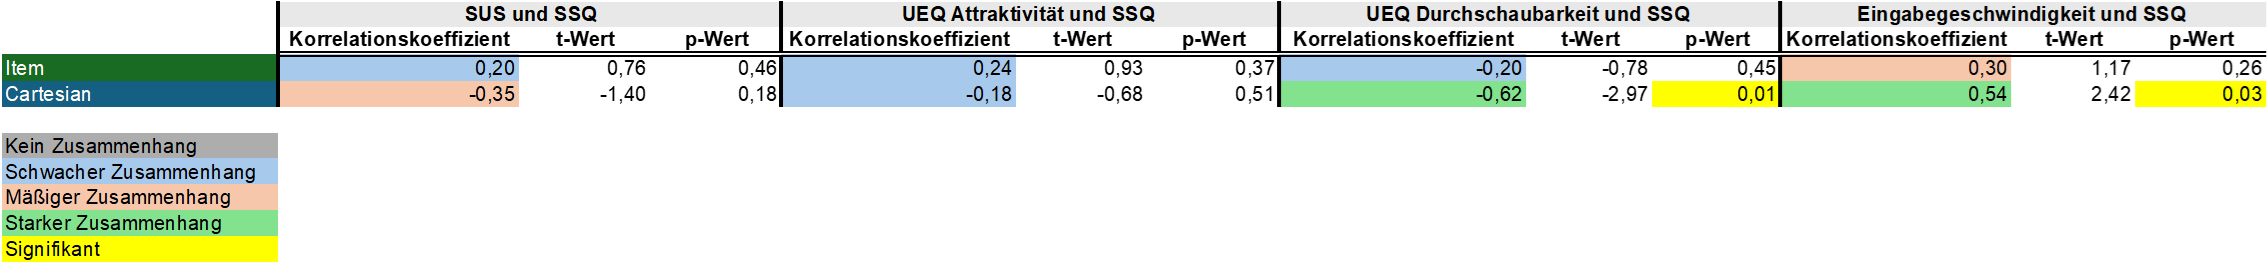
\includegraphics[width=0.95\textwidth]{images/Results/Korrelationen-SSQ.png}
    \caption{Zusammenhänge zwischen der Ergebnissen des SSQ und des SUS, des UEQ sowie der Eingabegeschwindigkeit}
    \label{fig:TableKorrelationenSSQ}
\end{figure}

Für die Korrelation zwischen SSQ und SUS ergab sich beim Item Scanning ein Korrelationskoeffizient von 0,17 (p-Wert = 0,53), während beim Cartesian Scanning ein Korrelationskoeffizient von -0,33 (p-Wert = 0,21) festgestellt wurde. 

Beim Vergleich des SSQ mit dem UEQ-Faktor Attraktivität ergab sich für das Item Scanning ein Korrelationskoeffizient von 0,24 (p-Wert = 0,36) und für das Cartesian Scanning ein Wert von -0,11 (p-Wert = 0,69). Für den UEQ-Faktor Durchschaubarkeit wurden Korrelationskoeffizienten von -0,20 (p-Wert = 0,45) für das Item Scanning und -0,66 (p-Wert = 0,01) für das Cartesian Scanning berechnet. Der Zusammenhang zwischen dem SSQ und der Interaktionsgeschwindigkeit war beim Item Scanning durch einen Korrelationskoeffizienten von 0,32 (p-Wert = 0,23) und beim Cartesian Scanning durch einen Korrelationskoeffizienten von 0,54 (p-Wert = 0,03) gekennzeichnet.

Darüber hinaus wurden die Zusammenhänge zwischen der Interaktionsgeschwindigkeit im technischen Abschnitt und der Bewertung der SUS sowie zwischen der Interaktionsgeschwindigkeit beider Abschnitte und der Bewertung des UEQ-Faktors Effizienz untersucht. Die Ergebnisse sind in \autoref{fig:TableKorrelationen} dargestellt. 

\begin{figure}[tbh]
    \centering
    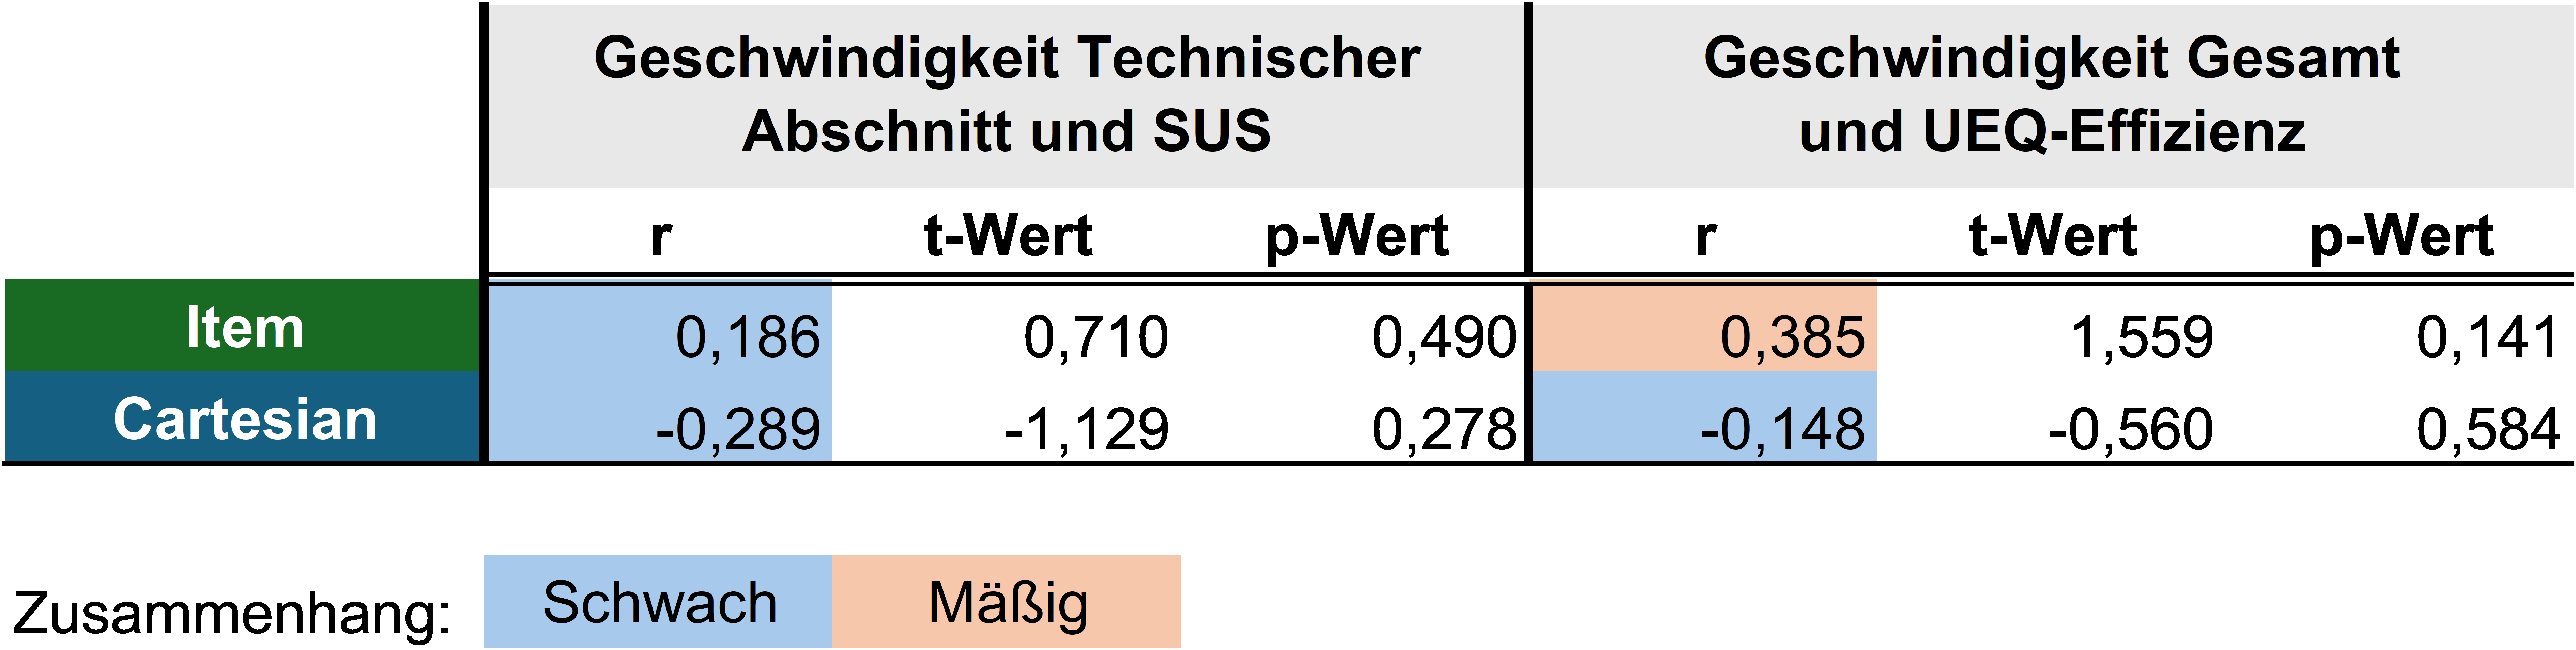
\includegraphics[width=0.95\textwidth]{images/Results/Korrelationen-Rest.png}
    \caption{Zusammenhang zwischen der Interaktionsgeschwindigkeit und der Usability/UX}
    \label{fig:TableKorrelationen}
\end{figure}

Die Korrelationskoeffizienten zwischen der Interaktionsgeschwindigkeit im technischen Abschnitt und dem UEQ-Faktor Effizienz betragen 0,19 (p-Wert = 0,49) für das Item Scanning und -0,29 (p-Wert = 0,28) für das Cartesian Scanning. Für die Interaktionsgeschwindigkeit über alle Abschnitte und den UEQ-Faktor Effizienz wurden Korrelationskoeffizienten von 0,38 (p-Wert = 0,14) für das Item Scanning und -0,15 (p-Wert = 0,58) für das Cartesian Scan errechnet.

\subsection{Qualitative Beobachtungen und Feedback der Teilnehmenden}

Neben den erhobenen Daten wurden während der Evaluation auch Beobachtungen notiert. Besonders auffällig war, dass viele Testpersonen gezielt Kopfbewegungen einsetzten, um das Cartesian Scanning zu beschleunigen oder kleine Fehler zu korrigieren. In \autoref{fig:kopfbewegungenCartesian} ist dargestellt, wie viele Personen gezielte Kopfbewegungen zu welchem Zweck einsetzten. Neun Personen setzten Kopfbewegungen für beide Zwecke ein, vier Personen ausschließlich zur Fehlerkorrektur und eine Person ausschließlich zur Beschleunigung. Zwei Personen setzten keine gezielten Kopfbewegungen ein.

\begin{figure}[tbh]
    \centering
    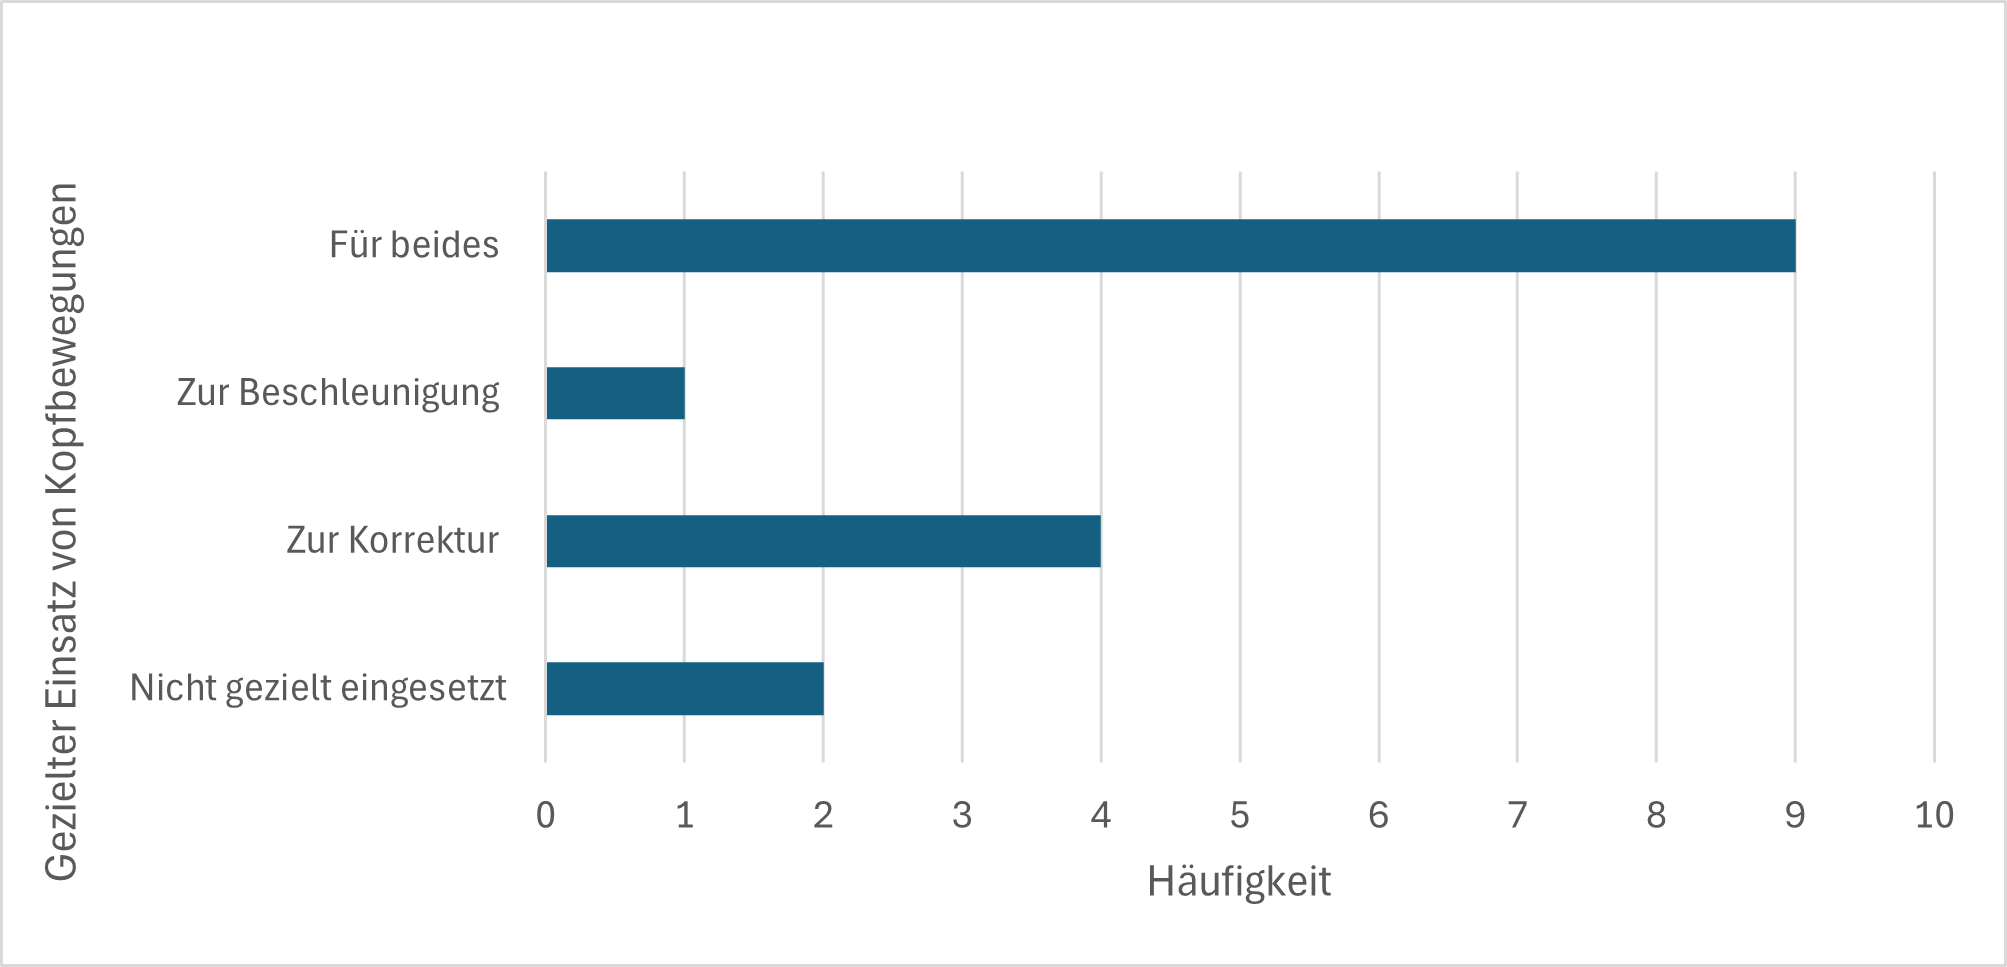
\includegraphics[width=0.8\textwidth]{images/Results/EinsatzKopfbewegungen-Cartesian.png}
    \caption{Einsatz gezielter Kopfbewegungen der Nutzenden beim Cartesian Scanning}
    \label{fig:kopfbewegungenCartesian}
\end{figure}

Darüber hinaus hatten die Teilnehmenden die Möglichkeit, freies Feedback zu den beiden Verfahren zu geben. Dieses Feedback wurde kategorisiert und wird im Folgenden zusammengefasst. 

\textbf{Einschätzungen zur Scan Rate:}

Die meisten Testpersonen äußerten sich bezüglich der Scan Rate der beiden Verfahren. \autoref{fig:scanrate} gibt die diesbezügliche Einschätzung der Testpersonen wider. Beim Item Scanning empfanden die meisten Testpersonen die Scan Rate als angenehm. Fünf Personen empfanden sie jedoch als zu langsam, eine Person als zu schnell und zwei Personen machten hierzu keine Angabe. Beim Cartesian Scanning empfand keine Person die Scanrate als zu schnell, während sechs Personen sie als angemessen beurteilten. Die meisten Personen gaben an, dass die Scan Rate zu langsam sei. Eine Person äußerte sich nicht.

\begin{figure}[tbh]
    \centering
    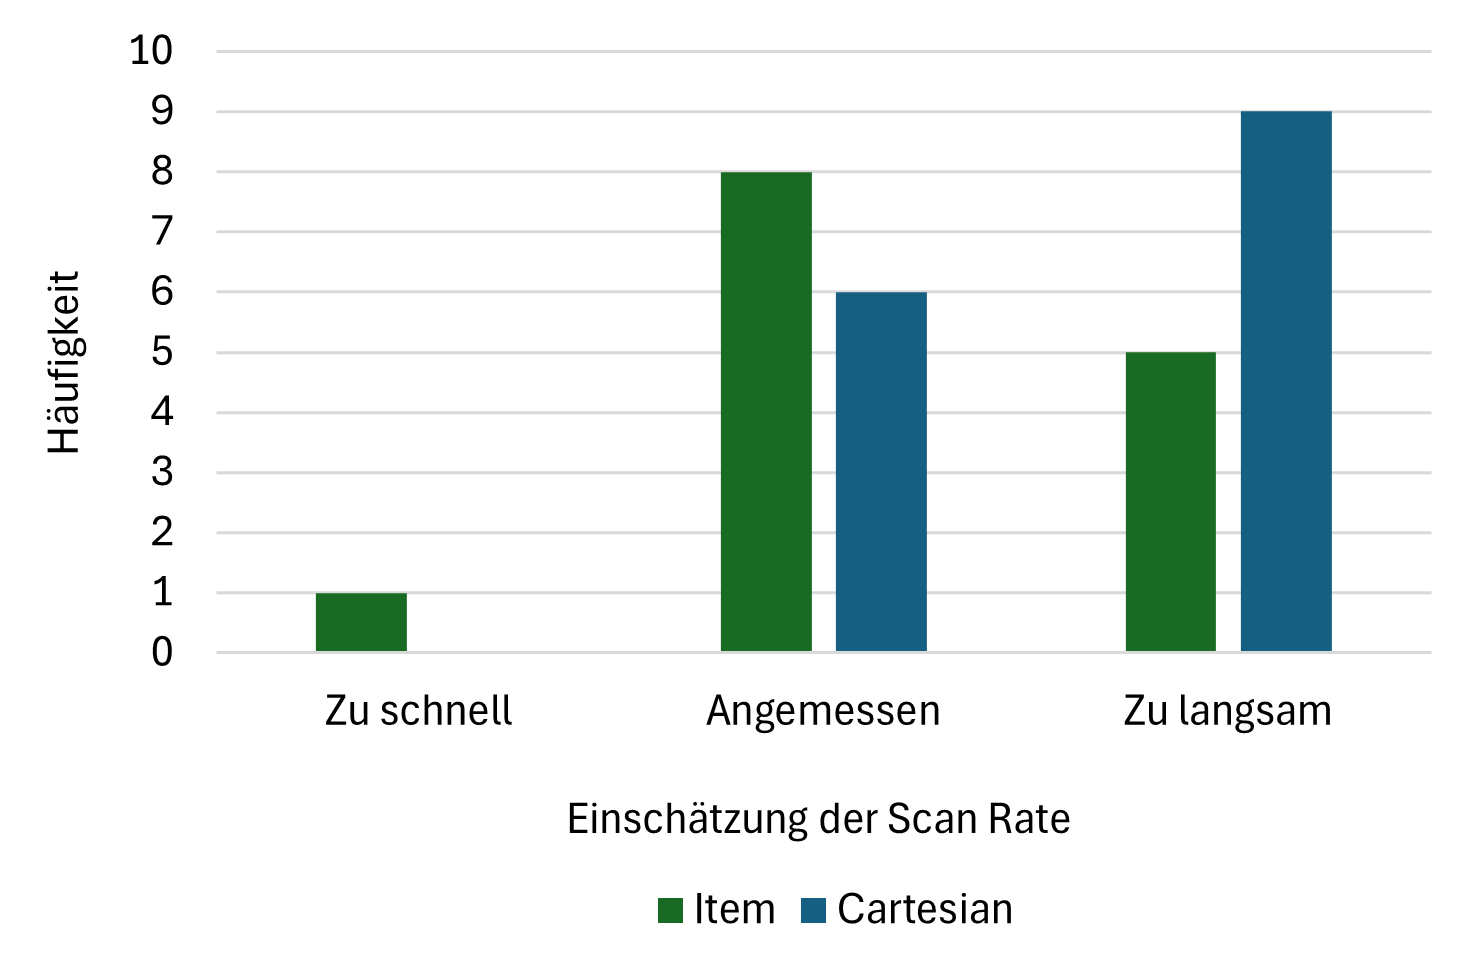
\includegraphics[width=0.75\textwidth]{images/Results/ScanRate.png}
    \caption{Einschätzungen zur Scan Rate beider Verfahren}
    \label{fig:scanrate}
\end{figure}

\textbf{Probleme und Kritik:}

Die meisten geäußerten Kritikpunkte bzw. Einordnungen der aufgetretenen Probleme bezogen sich auf das Item Scanning. Drei Testpersonen kritisierten die Scanning-Reihenfolge, die als willkürlich oder nicht nachvollziehbar empfunden wurde. Zudem wurde die Animation während des Item Scannings von einer Person als verwirrend beschrieben, da sie dazu führte, dass die Selektion teilweise zu früh erfolgte. Des Weiteren wurde von drei Personen bemängelt, dass das Menü (Navigation und HUD) zu weit oben im Sichtfeld positioniert war. Eine Person äußerte, dass Schwierigkeiten bei der Navigation aufgrund einer zu hohen Scan Rate auftraten. Eine weitere Person merkte an, dass im inhaltsbasierten Abschnitt versteckte Objekte durch das Verfahren „gespoilert“ wurden. Dies wurde als schade, aber nicht als ernsthaftes Problem angesehen. 

\textbf{Vorschläge für Verbesserungen:}

Die Testpersonen äußerten verschiedene Ideen zur Verbesserung der Verfahren. Beim Item Scanning wurde vorgeschlagen, beim ersten Objekt die Wartezeit etwas zu verlängern, da dieses leicht verpasst werden kann. Außerdem wurde vorgeschlagen, im Navigationsmenü eine Art „Cool Down“ einzuführen, um leichter mehrere Selektionen hintereinander durchführen zu können. Für das Cartesian Scanning wurde vorgeschlagen, die Zeit zu verkürzen, die benötigt wird, um den Schalter für den Moduswechsel gedrückt zu halten. Zwei Personen äußerten auch den Wunsch, die Geschwindigkeit der Linien dynamisch steuern zu können, um Wartezeiten zu reduzieren und das Verfahren effizienter zu gestalten. Außerdem wurde vorgeschlagen, die Scan Rate und die Farben für beide Verfahren individuell einstellbar zu gestalten.

\textbf{Positives Feedback und Aussagen zu Präferenzen zwischen den Verfahren:}

Die Testpersonen gaben auch Feedback zu Aspekten, die sie als positiv empfanden. Die Teilnehmenden beschrieben das Cartesian Scanning als einfacher und lobten die größere Kontrolle über das Verfahren. Es wurde auch betont, dass das Cartesian Scanning intuitiver sei. Es wurde außerdem von zwei Testpersonen für die bessere Navigation gelobt, da es einen schnelleren Wechsel des Blickwinkels ermöglichte. Eine Testperson gab an, dass das Cartesian Scanning zwar einfacher und individueller sei, das Item Scanning jedoch mehr Spaß mache. Auch andere Testpersonen bevorzugten das Item Scanning, da es als angenehmer empfunden wurde, insbesondere wegen der schnelleren Interaktionsgeschwindigkeit, der geringeren Fehleranfälligkeit und der optischen Gestaltung, die als augenschonender beschrieben wurde. 


